\documentclass[12pt,a4paper]{report}
\usepackage{dissertation}
\usepackage{blindtext}
\usepackage[colorinlistoftodos]{todonotes}
\usepackage{regexpatch}
\usepackage{subcaption}
\usepackage{listings}  % para utilizar blocos de texto verbatim no estilo 'listings'
%paramerização mais vulgar dos blocos LISTING - GENERAL
\lstset{
	basicstyle=\scriptsize, %o tamanho das fontes que são usadas para o código
	numbers=left, % onde colocar a numeração da linha
	numberstyle=\tiny, %o tamanho das fontes que são usadas para a numeração da linha
	numbersep=5pt, %distancia entre a numeração da linha e o codigo
	breaklines=true, %define quebra automática de linha
    frame=tB,  % caixa a volta do codigo
	mathescape=true, %habilita o modo matemático
	escapeinside={(*@}{@*)} % se escrever isto  aceita tudo o que esta dentro das marcas e nao altera
}
%
\definecolor{codegreen}{rgb}{0,0.6,0}
\definecolor{codegray}{rgb}{0.5,0.5,0.5}
\definecolor{codepurple}{rgb}{0.58,0,0.82}
\definecolor{backcolour}{rgb}{0.98,0.98,0.95}
\lstset{%
    language=Python,                     % Sets the language of the code
    backgroundcolor=\color{backcolour},  % Background color of the code
    commentstyle=\color{codegreen},      % Color of comments
    keywordstyle=\color{magenta},        % Color of keywords
    numberstyle=\tiny\color{codegray},   % Style of the line numbers
    stringstyle=\color{codepurple},      % Style of strings
    basicstyle=\footnotesize,            % Basic style for code
    numbers=left,                        % Line numbers on the left
    stepnumber=1,                        % Line numbering step
    numbersep=5pt,                       % Space between line numbers and code
    showspaces=false,                    % Do not show spaces
    showstringspaces=false,              % Do not underline spaces in strings
    showtabs=false,                      % Do not show tabs
    frame=tb,                            % Adds a frame above and below the code
    tabsize=2,                           % Default tab size
    captionpos=b,                        % Disables captions
    abovecaptionskip=0pt,                % Removes padding above captions
    belowcaptionskip=0pt,                % Removes padding below captions
    breaklines=true,                     % Enable automatic line breaking
    breakatwhitespace=false,             % Break lines not only at whitespace
    title=\lstname,                      % Show filename if \lstinputlisting is used
    escapeinside={\#*}{*)},              % Allows LaTeX within code
    inputencoding=utf8,                  % Encoding of the input file
    extendedchars=true,                  % Allows usage of extended characters
    literate=                            % Handles special characters
        {á}{{\'a}}1 {ã}{{\~a}}1 {é}{{\'e}}1 {ú}{{\'u}}1 {í}{{\'i}}1 {ó}{{\'o}}1 
        {õ}{{\~o}}1 {ç}{{\c{c}}}1 {à}{{\`a}}1 {ê}{{\^e}}1 {â}{{\^a}}1 
        {Ú}{{\'U}}1 {Í}{{\'I}}1
}

\lstdefinelanguage{Yaml}{
  keywords={true,false,null,y,n},
  keywordstyle=\color{blue}\bfseries,
  basicstyle=\ttfamily,
  sensitive=false,
  comment=[l]{\#},
  morecomment=[s]{/*}{*/},
  commentstyle=\color{gray}\ttfamily,
  stringstyle=\color{brown},
  morestring=[b]',
  morestring=[b]",
  literate=*{:}{{\textcolor{red}{:}}}1 % Colon highlighting
           {,}{{\textcolor{red}{,}}}1 % Comma highlighting
           {\{}{{\textcolor{red}{\{}}}1 % Left brace
           {\}}{{\textcolor{red}{\}}}}1 % Right brace
           {[}{{\textcolor{red}{[}}}1 % Left bracket
           {]}{{\textcolor{red}{]}}}1 % Right bracket
}
\usepackage[style=ieee, maxnames=3, minnames=1, backend=bibtex]{biblatex} % Modern bibliography management
\addbibresource{dissertation_clean.bib} % Link to the bibliography file


% Make todo notes inline by default
\makeatletter
\xpatchcmd{\@todo}{\setkeys{todonotes}{#1}}{\setkeys{todonotes}{prepend,color=blue!20!white,inline,#1}}{}{}
\makeatother


\makeglossaries
\makeindex

\logo{EE}{School of Engineering}{}
\logoB{EE}{School of Engineering}{}

\author{Fábio Lucas Pereira Carneiro}

\titleA{Luminosity Calibrations at the CERN\\Compact Muon Solenoid Experiment}

\masters{Master’s in Physics Engineering}
\area{Specialization in Physics Information}
\supervisor{Nuno Filipe Da Silva Fernandes De Castro}
\cosupervisor{Andres Guillermo Delannoy Sotomayor}

% COMMANDS
\newcommand{\ilum}{\ensuremath{\mathcal{L}}}
\newcommand{\Ilum}{\ensuremath{L}}
\newcommand*{\vv}[1]{\vec{\mkern0mu#1}}
\newcommand{\note}[2][]{\todo[color=green!20!white,#1]{#2}}
\newcommand{\fixme}[2][]{\todo[color=red!20!white,#1]{#2}}

% \bibpunct[,]{(}{)}{;}{a}{,}{,}
\begin{document}
\setlength{\parindent}{0em}

%-- Covers
\input{covers/Covers}

%-- Document setup
\newgeometry{right=25mm, left=25mm, top=25mm, bottom=25mm}
\pagenumbering{roman}

\setlength{\parskip}{0pt}
\setlength{\parindent}{1.5em}

%-- Preamble
\chapter*{Copyright and Terms of Use for Third Party Work}
\setlength{\parskip}{1em}
\noindent
This dissertation reports on academic work that can be used by third parties as long as the internationally accepted standards and good practices are respected concerning copyright and related rights.

\noindent
This work can thereafter be used under the terms established in the license below.

\noindent
Readers needing authorization conditions not provided for in the indicated licensing should contact the author through the RepositóriUM of the University of Minho.

\section*{License granted to users of this work:}

% \textit{[Caso o autor pretenda usar uma das licenças Creative Commons, deve escolher e deixar apenas um dos seguintes ícones e respetivo lettering e URL, eliminando o texto em itálico que se lhe segue. Contudo, é possível optar por outro tipo de licença, devendo, nesse caso, ser incluída a informação necessária adaptando devidamente esta minuta]}

\noindent
\includegraphics[]{images/CCBY.png}
\\
\textbf{CC BY}
\\
\url{https://creativecommons.org/licenses/by/4.0/}
% \textit{[Esta licença permite que outros distribuam, remixem, adaptem e criem a partir do seu trabalho, mesmo para fins comerciais, desde que lhe atribuam o devido crédito pela criação original. É a licença mais flexível de todas as licenças disponíveis. É recomendada para maximizar a disseminação e uso dos materiais licenciados.]}

%--

% \noindent
% \includegraphics[]{images/CCBYSA.png}
% \\
% \textbf{CC BY-SA}
% \\
% \url{https://creativecommons.org/licenses/by-sa/4.0/}
% \textit{[Esta licença permite que outros remisturem, adaptem e criem a partir do seu trabalho, mesmo para fins comerciais, desde que lhe atribuam o devido crédito e que licenciem as novas criações ao abrigo de termos idênticos. Esta licença costuma ser comparada com as licenças de software livre e de código aberto «copyleft». Todos os trabalhos novos baseados no seu terão a mesma licença, portanto quaisquer trabalhos derivados também permitirão o uso comercial. Esta é a licença usada pela Wikipédia e é recomendada para materiais que seriam beneficiados com a incorporação de conteúdos da Wikipédia e de outros projetos com licenciamento semelhante.]}

% %--

% \noindent
% \includegraphics[]{images/CCBYND.png}
% \\
% \textbf{CC BY-ND}
% \\
% \url{https://creativecommons.org/licenses/by-nd/4.0/}
% \textit{[Esta licença permite que outras pessoas usem o seu trabalho para qualquer fim, incluindo para fins comerciais. Contudo, o trabalho, na forma adaptada, não poderá ser partilhado com outras pessoas e têm que lhe ser atribuídos os devidos créditos.]}

% %--

% \noindent
% \includegraphics[]{images/CCBYNC.png}
% \\
% \textbf{CC BY-NC}
% \\
% \url{https://creativecommons.org/licenses/by-nc/4.0/}
% \textit{[Esta licença permite que outros remisturem, adaptem e criem a partir do seu trabalho para fins não comerciais, e embora os novos trabalhos tenham de lhe atribuir o devido crédito e não possam ser usados para fins comerciais, eles não têm de licenciar esses trabalhos derivados ao abrigo dos mesmos termos.]}

% %--

% \noindent
% \includegraphics[]{images/CCBYNCSA.png}
% \\
% \textbf{CC BY-NC-SA}
% \\
% \url{https://creativecommons.org/licenses/by-nc-sa/4.0/}
% \textit{[Esta licença permite que outros remisturem, adaptem e criem a partir do seu trabalho para fins não comerciais, desde que lhe atribuam a si o devido crédito e que licenciem as novas criações ao abrigo de termos idênticos.]}

% %--

% \noindent
% \includegraphics[]{images/CCBYNCND.png}
% \\
% \textbf{CC BY-NC-ND}
% \\
% \url{https://creativecommons.org/licenses/by-nc-nd/4.0/}
% \textit{[Esta é a mais restritiva das nossas seis licenças principais, só permitindo que outros façam download dos seus trabalhos e os compartilhem desde que lhe sejam atribuídos a si os devidos créditos, mas sem que possam alterá- los de nenhuma forma ou utilizá-los para fins comerciais.]}

\setlength{\parskip}{0em}
\input{preamble/Acknowledgements}
\input{preamble/StatementofIntegrity}
\chapter*{Abstract}

The quest to understand the fundamental nature of the universe drives the field of particle physics, centered around the Standard Model (SM), which describes the fundamental particles and three of the four known forces: electromagnetism, the weak force, and the strong force. Despite its success in explaining a wide range of phenomena, the SM does not address some of the most profound questions in physics, such as the nature of dark matter, the origin of mass hierarchies, and the unification of forces. Probing the SM with precision measurements is essential for uncovering potential new physics beyond the current theoretical framework.

Particle colliders like the Large Hadron Collider (LHC) at CERN are at the forefront of this exploration, where measurements of cross sections are a crucial part of the physics program that tests the SM’s predictions. A cross section quantifies the likelihood of specific particle's interactions, and accurate luminosity measurements are fundamental to determining these cross sections. Luminosity, \(\mathcal{L}\), is proportional to the rate of collisions, and thus any uncertainty in \(\mathcal{L}\) translates into uncertainties in the cross sections, affecting the reliability of the conclusions drawn from experimental data.

This thesis presents the calibration and measurement of luminosity for the 2023 proton-proton collision data-taking period at a center-of-mass energy of 13.6 TeV with the CMS experiment. The absolute luminosity scale is established using the van der Meer (vdM) scan methodology, a technique that involves scanning the particle beams across each other to measure their overlap and calibrate the visible cross sections of the luminometers. A series of detectors were employed to provide real-time luminosity measurements, with systematic corrections and stability analyses ensuring consistent and accurate results

The final integrated luminosity was measured as 32.74 fb\textsuperscript{-1} with a total uncertainty of 1.28\%, representing the best preliminary luminosity results achieved by CMS. In addition to the experimental efforts, substantial software improvements were made to the codebases used in the analysis. These advancements enhanced data processing efficiency and streamlined the calibration workflow, enabling more rapid and reliable analysis iterations.

\paragraph{Keywords} CERN, CMS, Luminosity, van der Meer

\cleardoublepage

\chapter*{Resumo}

A busca por compreender a natureza fundamental do universo impulsiona o campo da física de partículas, centrado no Modelo Padrão (SM), que descreve as partículas fundamentais e três das quatro forças conhecidas: o electromagnetismo, a força fraca e a força forte. Apesar do seu sucesso em explicar uma ampla gama de fenómenos, o SM não aborda algumas das questões mais profundas da física, como a natureza da matéria escura, a origem das hierarquias de massa e a unificação das forças. Provar o SM com medições de alta precisão é essencial para descobrir novas possíveis físicas para além do atual quadro teórico.

Colisores de partículas como o Grande Colisor de Partículas (LHC) no CERN estão na vanguarda desta exploração, onde as medições das secções eficazes são cruciais para testar as previsões do SM. A secção eficaz quantifica a probabilidade de interações de específicas partículas, e medições precisas da luminosidade são fundamentais para determinar estas secções eficazes. A luminosidade, \(\mathcal{L}\), influencia diretamente a taxa de colisões, e, portanto, qualquer incerteza em \(\mathcal{L}\) traduz-se em incertezas nas secções eficazes, afetando a fiabilidade das conclusões extraídas dos dados experimentais.

Esta tese foca-se na calibração e medição da luminosidade para o período de 2023 que corresponde a colisões protão-protão a uma energia de centro de massa de 13,6 TeV na experiência CMS. A escala absoluta da luminosidade é estabelecida utilizando a metodologia de scans de van der Meer (vdM), uma técnica que baseada no scan dos feixes de partículas entre si para medir a sobreposição e calibrar as secções eficazes visíveis dos luminómetros. Foi empregue uma série de detectores para fornecer medições de luminosidade em tempo real, com correções sistemáticas e análises de estabilidade a garantir resultados consistentes e precisos.

A medição final da luminosidade integrada foi de 32.74 fb\textsuperscript{-1} com uma incerteza total de 1.28\%, o melhor resultado preliminar alcançado pelo CMS. Além dos esforços experimentais, foram feitas melhorias no software utilizado nas análises. Estes avanços aumentaram a eficiência do processamento de dados e simplificaram o fluxo de trabalho da calibração, permitindo iterações de análise mais rápidas e fiáveis.

\paragraph{Palavras-chave} CERN, CMS, Luminosidade, van der Meer

\cleardoublepage


\phantomsection
% \listoftodos
\tableofcontents

\cleardoublepage
\listoffigures

% List of tables
\renewcommand*{\listtablename}{List of Tables}
\listoftables
\clearpage

% Acronyms
\printglossary[type=\acronymtype,nonumberlist, title={Acronyms}]

% Glossary
\printglossary[title={Glossary}, nonumberlist]

\cleardoublepage
\pagenumbering{arabic}

\chapter{Introduction}

\newacronym{sm}{SM}{Standard Model}

The quest to understand the universe at its most fundamental level lies at the heart of particle physics. Scientists in this field aim to explore the properties, behaviors, and interactions of elementary particles. Particle physics seeks to answer fundamental questions about the universe, such as the origin of mass, the nature of dark matter, and the unification of forces.

The \acrfull{sm} is a theoretical framework that describes the fundamental particles and their interactions, excluding gravity. It encompasses three of the four known fundamental forces: electromagnetism, the weak nuclear force, and the strong nuclear force. It also incorporates the Higgs mechanism, giving elementary particles their mass. The particles in the Standard Model include quarks, leptons, gauge bosons, and the Higgs boson. Quarks and leptons are the building blocks of matter, while gauge bosons mediate the interactions between these particles.

Particle colliders, key instruments in this research process, accelerate and collide particles to reveal new insights through the analysis of the byproducts of such collisions. These events or processes are characterized by their cross sections. Often denoted as $\sigma$ and measured in units of area, the cross section of an event quantifies the probability of it occurring in a particle interaction. By comparing observed cross sections with those predicted by the \acrshort{sm}, physicists can test the validity of the model and potentially identify discrepancies indicating new physics beyond the \acrshort{sm}.

The performance of particle colliders is determined by two key parameters: the center-of-mass energy and the luminosity, $\mathcal{L}$. While the center-of-mass energy defines the energy scale of the collisions, the luminosity quantifies the rate at which particles interact, directly determining the total amount of events that a collider can produce over a given time period. The instantaneous luminosity, \ilum, is a proportionality constant that relates the rate of an event, $R$, to its cross section, $R = \ilum \sigma$. The colossal importance of precise cross section measurements, from which the \acrshort{sm} can be probed, sparks the need for precise measurements of the luminosity and fuels the motivation behind this thesis.

\section{The Large Hadron Collider}
\label{subsec:lhc}

\newacronym{cern}{CERN}{European Organization for Nuclear Research}
\newacronym{lhc}{LHC}{Large Hadron Collider}
\newacronym{ip}{IP}{Interaction Points}
\newacronym{cms}{CMS}{Compact Muon Solenoid}

The \acrfull{lhc} at the \acrfull{cern} is a monumental particle accelerator \cite{lhc}. It's an underground facility spanning the border of France and Switzerland. Its purpose is to accelerate particles beams, one clockwise and the other counterclockwise, and make them collide at high energies to probe the fundamental properties of matter. The collisions happen at four main \acrfull{ip} that correspond to the four main experiments:
\begin{itemize}
	\item \acrfull{cms}: A general-purpose detector designed to investigate a wide range of physics, including the study of the Higgs boson, precision probes of the \acrshort{sm}, and searches for new phenomena. \acrshort{cms} is located at \acrshort{ip} 5.
	\item A Toroidal LHC Apparatus (ATLAS): The second general-purpose detector at the \acrshort{lhc}. Shares similar goals with \acrshort{cms} and is located at the opposite side of the \acrshort{lhc} ring. ATLAS is located at \acrshort{ip} 1.
	\item A Large Ion Collider Experiment (ALICE): A dedicated heavy-ion detector designed to study the physics of strongly interacting matter at extreme energy densities, such as quark-gluon plasma. ALICE is located at \acrshort{ip} 2.
	\item Large Hadron Collider beauty (LHCb): A detector designed to study the differences between matter and antimatter by studying particle interactions involving the "beauty" quark. LHCb is located at \acrshort{ip} 8.
\end{itemize}

The \acrshort{lhc} stands as the world's largest particle accelerator, capable of accelerating protons to a maximum energy of 6.8 TeV. It started operations in 2009 and has since been a cornerstone of particle physics research with its most notable achievement being the discovery of the Higgs boson in 2012 \cite{HiggsDiscovery}. Every \acrshort{lhc} fill is assigned a unique number each time a new beam is injected into the collider.

% Runs, correspond to <insert_here_run_definition> and are also given a unique number. Fill and runs lenghts can vary as well as the number of runs within a given fill.

The \acrshort{lhc} operates according to a planned schedule, which is meticulously planned and updated, when needed, to ensure the success of its experimental programs and upgrades. The current schedule, as shown in \autoref{fig:lhc_schedule}, outlines the activities for Run 3, which is expected to continue until 2025.


\begin{figure}[!htb]
    \centering
    \includegraphics[width=0.8\textwidth]{images/assets/lhc_schedule.png}
    \caption[LHC Run 3 schedule]{The LHC schedule for Run 3, detailing the operational plan until 2025 (from \textit{Ref.} \cite{LHCSchedule}).}
    \label{fig:lhc_schedule}
\end{figure}

\subsection{Accelerator Complex}
\label{subsec:acc_complex}

\newacronym{bcid}{BCID}{Bunch Crossing Identifier}

The \acrshort{lhc} is only the final stage of a complex series of accelerators that prepare the particles for collision. Before protons are injected into the \acrshort{lhc}, they pass through a sequence of smaller accelerators that progressively increase their energy. This series of accelerators forms the comprehensive CERN accelerator complex, as shown in Figure~\ref{fig:cern_acc_complex}.

\begin{figure}[h]
	\centering
	\includegraphics[width=\textwidth]{images/assets/cern_accelerator_complex.png}
	\caption[CERN Accelerator Sequence]{Diagram of the \acrshort{cern} Accelerator Sequence (from \textit{Ref.} \cite{cern-accelerator-complex}): Sequence of accelerators that prepare protons for injection into the \acrshort{lhc}. The path that protons follow can be traced from Linac4, to BOOSTER, to the PS, to the SPS, and finally to the LHC. Highlighed in yellow are the four main experiments at the \acrshort{lhc}. The LINAC3 and LEIR, whose purpose is to provide ions for the LHC, are also shown.}
	\label{fig:cern_acc_complex}
\end{figure}

The \acrshort{cern} accelerator complex begins its operations with the Linear Accelerator 4 (Linac4) \cite{Linac4}, which, has served as the primary source for proton beams since 2020. Linac4 boosts the energy of negative hydrogen ions (H$^-$) --- that is, hydrogen atoms with an additional electron --- to 160 million MeV. Using radio frequency (RF) cavities, Linac4 charges a series of conductors in an alternating positive and negative manner, causing the particles to be accelerated. Before being pulsed through the accelerator, the H$^-$ ions are squeezed into a tight beam using quadrupole magnets. These ions are then readied to enter the Proton Synchrotron Booster (PSB), where they lose their two extra electrons and only the protons remain. The PSB further accelerates these protons to 2 GeV, before they proceed to the Proton Synchrotron (PS). At the PS, the proton energy is increased to 26 GeV. Subsequently, the protons are directed to the Super Proton Synchrotron (SPS), where their energy reaches 450 GeV. Finally, these protons are conveyed to the \acrshort{lhc}, where each beam is accelerated to an energy of 6.8 TeV.

In addition to protons, the \acrshort{lhc} also accelerates heavy ions, namely, lead and xenon nuclei. These ions initially enter the Linear Accelerator 3 (Linac3). Once gathered, they are sped up in the Low Energy Ion Ring (LEIR) and eventually follow the same trajectory as the protons to reach their maximum energy.


\subsection{Particle Beams}
\label{subsec:particle_beams_lhc}

In the \acrshort{lhc}, particles are grouped into bunches, each containing approximately $10^{11}$ protons at the start of a physics fill. These bunches travel around a 27 km ring at nearly the speed of light, resulting in an orbiting frequency of approximately 11245.5 Hz. The RF cavities that accelerate the bunches operate with an oscillating electric field at a frequency of 400 MHz, creating a total of 35640 RF buckets, each spaced 2.5 ns apart. This arrangement is demanding, as it requires a high degree of timing resolution for any detector system aiming to obtain measurements per bucket. Buckets are grouped into sets of 10, with only the first bucket nominally filled with particles. This grouping increases the spacing between filled particle bunches to 25 ns. These bunch slots are referred to as bunch crossings and assigned a unique number called \acrfull{bcid}, ranging from 1 to 3564.

Each \acrshort{lhc} fill has a well-defined filling scheme. This scheme provides information on parameters such as the bunch spacing, the number of filled bunches per beam, the number of collisions at each \acrshort{ip}, and the number of consecutive filled bunches, also known as a train, among others. The filling scheme heavily influences the physics conditions of the fill, dictating the experimental environment and collision dynamics. Special fills and given identified by a counter. may be requested to address a unique number that is incremented every time  experimental conditions in order to achieve the desired physics goals.


\subsection{Compact Muon Solenoid Experiment}
\label{subsec:cms}

The \acrlong{cms} \cite{TheCMSCollaboration_2008}, is a multi-purpose detector operating at the \acrshort{lhc}, designed to operate under high instantaneous luminosity conditions. These conditions require radiation resistance, sub-detector systems with high granularity, and an intricate readout and trigger system. To fulfill its requirements the \acrshort{cms} apparatus is composed of a series of subsystems. Figure~\ref{fig:cms_detector} shows a schematic of the \acrshort{cms} detector and its subsystems. \acrshort{cms} is located underground close to the French village of Cessy, between Lake Geneva and the Jura mountains. Its coordinate system in relation to the \acrshort{lhc} ring is illustrated in Figure~\ref{fig:cms_system_coordinates}.

\begin{figure}[h]
	\centering
	\makebox[\textwidth][c]{%
		\begin{minipage}[b]{0.5\textwidth}
			\centering
			\includegraphics[width=\textwidth]{images/assets/cms_detector.png}
			\subcaption{}
			\label{fig:cms_detector}
		\end{minipage}
		\hspace{0.05\textwidth}
		\begin{minipage}[b]{0.5\textwidth}
			\centering
			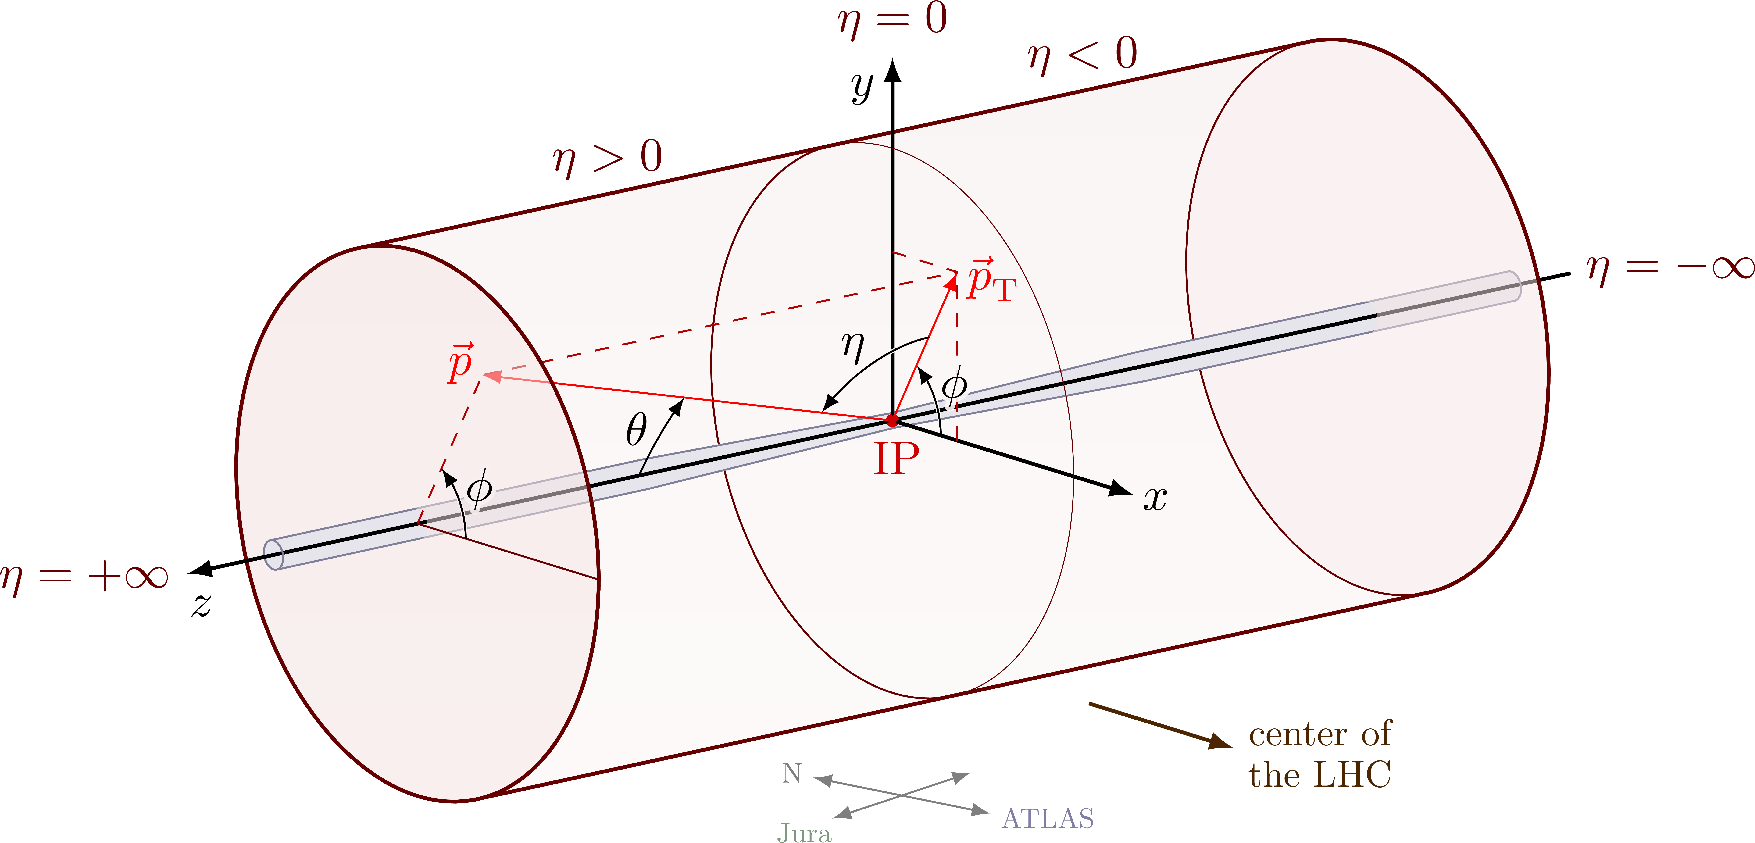
\includegraphics[width=\textwidth]{images/assets/cms_system_coordinates.pdf}
			\subcaption{}
			\label{fig:cms_system_coordinates}
		\end{minipage}
	}
	\caption[CMS detector and coordinate system]{(a) Schematic of the \acrshort{cms} detector outlining its subsystems (adapted from \textit{Ref.} \cite{CERN:39040}). (b) Diagram of the \acrshort{cms} coordinate system as seen with the \acrshort{lhc} cylinder in the background. The $x$-axis points radially to the center of the \acrshort{lhc} ring, the $y$-axis points upwards, and the $z$-axis points along the beam direction. The azimuthal angle, $\phi$, is measured from the $x$-axis to the $\vv{p}_T$ vector in the $x-y$ plane. The polar angle, $\theta$, is measured from the $z$-axis to the $\vv{p}$ vector. Each zone is labeled with the corresponding pseudorapidity, $\eta$, defined as $\eta = - \ln \tan (\theta / 2)$.}
	\label{fig:cms_images}
\end{figure}

As stated in Section~\ref{subsec:lhc}, the \acrshort{cms} physics program encompasses a wide range of topics. From the study of the Higgs boson, to continuously probing the \acrshort{sm} through precision measurements, to searching for new physics phenomena at high energy scales. The detector is built from the conjunction of multiple layers of subsystems, each with a dedicated focus on measuring specific products of the collision events as they traverse the detector. The subsystems, from the center outwards, are depicted in Figure~\ref{fig:cms_slice}.

\begin{figure}[h]
	\centering
	\includegraphics[width=\textwidth]{images/assets/cms_slice.png}
	\caption[Tranverse slice of CMS detector]{Transverse slice of the \acrshort{cms} detector (from \textit{Ref.} \cite{Barney:2120661}). The subsystems are shown from the center outwards: the silicon tracker, the electromagnetic calorimeter, the hadronic calorimeter, and the muon system.}
	\label{fig:cms_slice}
\end{figure}

\newacronym{ecal}{ECAL}{Electromagnetic Calorimeter}
\newacronym{hcal}{HCAL}{Hadronic Calorimeter}

The part of the detector closest to the beam pipe is the silicon tracker. This subsystem is composed of silicon sensors that track the paths of charged particles as they ionize the silicon while moving through it. Influenced by the \acrshort{cms} magnet, the curvature of these particles' paths provides crucial information for calculating their momentum, with more curved paths indicating lower momentum. The tracker can reconstruct the paths of charged particles, including electrons, hadrons, and high-energy muons. Immediately following the tracker are the \acrshort{cms} calorimeters: the \acrfull{ecal} and the \acrfull{hcal}. These calorimeters measure the energy of particles by stopping them and measuring the energy they deposit. The \acrshort{ecal}, composed of lead tungstate crystals, detects electrons and photons by scintillating upon interaction with these particles. Photodetectors, designed to operate within the high magnetic field, are attached to the back of each crystal to detect the scintillation light and convert it to an electrical signal that is then amplified and analyzed. The \acrshort{hcal} measures the energy of hadrons, which are particles made of quarks and gluons, such as protons and neutrons. Additionally, it allows for the indirect measurement of non-interacting particles, such as neutrinos, through missing transverse energy, which represents the imbalance in the sum of transverse momentum of the particles in the event. The \acrshort{hcal} is constructed with alternating layers of absorber and scintillating materials, producing rapid light pulses when particles pass through. It is organized into several sections: the barrel (HB), outer barrel (HO), endcap (HE), and forward (HF) sections. Muons, heavy cousins of electrons, are the particles most likely to pass through the calorimeters and reach the muon system. The muon system is the outermost layer of the \acrshort{cms} detector and is designed to detect muons. It is composed of three types of detectors: Drift Tubes (DT), Cathode Strip Chambers (CSC), and Resistive Plate Chambers (RPC). Detailed information on \acrshort{cms} subsystems can be found in \cite{CERN-LHCC-2020-004}.

\section{Luminosity}
\label{sec:luminosity}

Luminosity is essential in particle physics research for two key reasons. First, accurate measurements of instantaneous luminosity are crucial for tracking the performance of both the accelerator and its associated detectors \cite{PhysRevAccelBeams.21.102801}. Second, integrated luminosity often represents the primary source of uncertainty in numerous cross-section measurements \cite{cms2022measurement, sirunyan2019measurement}. This section provides a detailed overview of the concept of luminosity.

\subsection{Instantaneous and Integrated Luminosity}
\newacronym{sbil}{SBIL}{Single Bunch Instantaneous Luminosity}

Luminosity is defined as the ratio between the rate of events, $R$, and the cross-section of a given process, $\sigma$:
\begin{equation}
    \label{eq:inst-luminosity}
    \mathcal{L} = \frac{R}{\sigma}
\end{equation}
$\mathcal{L}$ has then units of $[\mathrm{area}]^{-1} [\mathrm{time}]^{-1}$ where cm$^{-2}$s$^{-1}$ or fb$^{-1}$s$^{-1}$ are common units ($1$ barn  $= 10^{-28}$ m$^{-2}$). Integrating over a given time interval, $t_2 - t_1$, yields the integrated luminosity, $L$:
\begin{equation}
    \label{eq:int-luminosity}
    L = \int_{t_1}^{t_2} \mathcal{L} dt = \int_{t_1}^{t_2} \frac{R}{\sigma} dt = \frac{N}{\sigma}
\end{equation}
It follows that $L$ is proportional to the number of events, $N$, produced in the collider.

From \autoref{eq:int-luminosity} it can be seen that luminosity can be measured if the cross-section of a given process is known. This is the case for lepton colliders, where the ``candle" process $e^+ e^- \rightarrow e^+ e^-$ is used to measure luminosity \cite{Burkhardt:1056691}. However, for hadron colliders, which involve collisions of particles made of quarks, such as protons, this approach is not feasible due to the large uncertainties in the calculation of cross-sections. Another approach is to measure luminosity using machine parameters, as described in the next section.

\subsection{Luminosity from Machine Parameters}
\label{subsec:luminosity_from_machine_parameters}

The \acrfull{sbil}, $\mathcal{L}_b$, can be measured using the collider's machine parameters \cite{Burkhardt:1056691}.
\begin{figure}[h]
    \centering
    \includegraphics[width=0.8\textwidth]{images/assets/bunch_crossing.png}
    \caption[Bunch crossing illustration]{Bunch crossing illustration (from \textit{Ref.} \cite{Burkhardt:1056691}).}
    \label{fig:bunch_crossing}
\end{figure}
For colliding bunches containing $N_1$ and $N_2$ particles respectively, the expected value of $\mathcal{L}_b$ is given by the following equation:
\begin{equation}
    \label{eq:sbil-machine-params}
    \mathcal{L}_b = \frac{N_1 N_2 f_{rev}}{A_{eff}}
\end{equation}
In this equation, $f_{rev}$ represents the orbiting frequency around the \acrshort{lhc}, as described in \autoref{subsec:particle_beams_lhc}, and $A_{eff}$ is the effective transverse area where collisions occur, also referred to as the luminous region. If the transverse distribution of particles was uniform, $A_{eff}$ would be equivalent to the transverse bunch overlap. However, considering the transverse particle distributions $\rho_1$ for bunch 1 and $\rho_2$ for bunch 2, the effective transverse area is defined by the overlap integral:
\begin{equation}
    \label{eq:effective-area}
    \frac{1}{A_{eff}} = 2 \int \rho_1(x,y) \rho_2(x,y) dxdy
\end{equation}
The factor of 2 corresponds to the Møller factor, which accounts for the fact that the two bunches are colliding at equal relativistic speeds and in opposite directions \cite{furman2003moeller}. Typically, it is assumed that these transverse particle distributions are uncoupled, meaning: 
\begin{equation}
    \begin{cases}
		\rho_1 \left(x, y \right) = \rho_{1x} \left( x \right) \rho_{1y} \left( y \right) \\
		\rho_2 \left(x, y \right) = \rho_{2x} \left( x \right) \rho_{2y} \left( y \right) \\
    \end{cases}\,.
\end{equation}
Under this assumption, the effective transverse area can be rewritten as:
\begin{equation}
    \label{eq:effective-area}
    \frac{1}{A_{eff}} = 2 \int \rho_{1x}(x) \rho_{2x}(x) dx \times \int \rho_{1y}(y) \rho_{2y}(y) dy = \frac{1}{W_{eff}} \times \frac{1}{H_{eff}}
\end{equation}
Here, $W_{eff}$ and $H_{eff}$ represent the effective transverse width and height, respectively. Substituting this back into equation \ref{eq:sbil-machine-params}, we get:
\begin{equation}
    \label{eq:sbil-machine-params-2}
    \mathcal{L}_b = 2 N_1 N_2 f_{rev} \int \rho_{1x}(x) \rho_{2x}(x) dx \times \int \rho_{1y}(y) \rho_{2y}(y) dy
\end{equation}
Further, assuming that the transverse particle distributions are Gaussian with widths $\sigma_{x1}$, $\sigma_{x2}$ and heights $\sigma_{y1}$, $\sigma_{y2}$, the equation becomes:
\begin{equation}
    \label{eq:sbil-machine-params-3}
    \mathcal{L}_b = 2 N_1 N_2 f_{rev} \int G_x (\sigma_{x1}) G_x (\sigma_{x2}) dx \times \int G_y (\sigma_{y1}) G_y (\sigma_{y2}) dy
\end{equation}
$G_i (\sigma)$ in this context is the Gaussian distribution with standard deviation $\sigma$ in the $i \in {x,y}$ direction and a mean of zero:
\begin{equation}
    \label{eq:gaussian-distribution}
    G_i (\sigma) = \frac{1}{\sigma \sqrt{2 \pi}} e^{-\frac{i^2}{2 \sigma^2}}
\end{equation}
Expanding the first integral:
\begin{equation}
	\label{eq:sbil-machine-params-4}
	\int G_x (\sigma_{x1}) G_x (\sigma_{x2}) dx = \frac{1}{2 \pi \sigma_{x1} \sigma_{x2}} \int e^{-\frac{x^2 \left( \sigma_{x1}^2 + \sigma_{x2}^2 \right)}{2 \sigma_{x1}^2 \sigma_{x2}^2}} dx
\end{equation}
and considering
\begin{equation}
	\int e^{-a x^2} dx = \sqrt{\frac{\pi}{2a}}
\end{equation}
equation \ref{eq:sbil-machine-params-4} can be simplified to:
\begin{equation}
	\label{eq:sbil-machine-params-5}
	\int G_x (\sigma_{x1}) G_x (\sigma_{x2}) dx = \frac{1}{2 \pi \sigma_{x1} \sigma_{x2}} \sqrt {\frac{\pi \sigma_{x1}^2 \sigma_{x2}^2}{\sigma_{x1}^2 + \sigma_{x2}^2}} = \frac{1}{2 \sqrt{\pi} \sqrt{\sigma_{x1}^2 + \sigma_{x2}^2}}
\end{equation}
Using the same approach for the second integral and substituting the results back into equation \ref{eq:sbil-machine-params-3}, we get: 
\begin{equation}
\label{eq:sbil-machine-params-6}
\mathcal{L}_b = \frac{N_1 N_2 f_{rev}}{2 \pi \Sigma_X \Sigma_Y}
\end{equation}
where $\Sigma_X = \sqrt{2\pi} W_{eff} = \sqrt{2\pi} \sqrt{\sigma_{x1}^2 + \sigma_{x2}^2}$ and $\Sigma_Y = \sqrt{2\pi} H_{eff} = \sqrt{2\pi} \sqrt{\sigma_{y1}^2 + \sigma_{y2}^2}$. In the case of round beams, the root-mean-squared widths of the horizontal and vertical beam profiles are equivalent to $\sqrt{\epsilon_{N} \beta^{*} / \gamma}$. $\gamma$ is the relativistic Lorentz factor, and $\beta^{*}$ corresponds to the value of the optical function $\beta$ at the IP. $\epsilon_{N}$ is the normalized transverse emittance, with a values of $3.75\mu m$ for the \acrshort{lhc} \cite{Brüning:782076}.

\subsection{Luminosity Calibration}
\label{subsec:luminosity_calibration}

Luminosity detectors, also called luminometers, are located at the \acrshort{ip}s of the \acrshort{lhc} and measure various observable quantities related to the rate of the collisions. Due to the differences between the luminometers, the nature of their recorded observables, and their location at the \acrshort{cms} cavern, each is assumed to only capture a fraction of the total collisions. This bias in the luminometers is accounted for by a detector-specific calibration factor, the visible cross-section, $\sigma_{vis}$. Using equations \ref{eq:inst-luminosity} and \ref{eq:sbil-machine-params-3} this calibration can be expressed as:
\begin{equation}
    \label{eq:vis-cross-section}
    \sigma_{vis} = \frac{2 \pi \Sigma_X \Sigma_Y R}{N_1 N_2 f_{rev}}
\end{equation}
Once calculated for each luminometer, the visible cross-section can be used to convert the measured rates to luminosity:
\begin{equation}
    \label{eq:luminosity-from-rates}
    \mathcal{L} = \frac{R}{\sigma_{vis}}
\end{equation}
In both these equations, $R$ represents the measured rate of events from a particular luminometer.

\subsection{Zero-Counting Method}
\label{subsec:zero-counting}

Due to the constraints in the read-out electronics of some luminometers, there's a chance that simultaneous particle hits might be recorded as a single event. This necessitates a more advanced approach to counting hits accurately. It is postulated that the distribution of the number of hits can be modeled by a Poisson distribution \cite{TheLHCbcollaboration_2014} with mean, $\mu$, that is proportional to luminosity.
\begin{equation}
    \label{eq:luminosity-from-hits}
    \mathcal{L}_b = \frac{\mu f_{rev}}{\sigma}
\end{equation}
The zero-counting method consists of calculating the probability that a luminometer records zero hits, $P_0$, regardless of the number of collisions that occur. This probability is given by the following equation:
\begin{equation}
    \label{eq:zero-counting}
    P_0 = \sum_{i=0}^{\infty} \frac{\mu^i e^{-\mu}}{i!} p^i = e^{-\mu(1-p)}
\end{equation}
$\mu$ is the mean number of hits per bunch crossing, also known as pileup, and $p$ is the probability that no observables are recorded in a bunch crossing with $i$ interactions. It then follows that luminosity is proportional to the natural logarithm of $P_0$:
\begin{equation}
    \label{eq:luminosity-from-hits-2}
    \mathcal{L}_b = \frac{\mu f_{rev}}{\sigma} = - \frac{\log (P_0)}{1-p} \frac{f_{rev}}{\sigma} = - \log (P_0) \frac{f_{rev}}{\sigma_{\mathrm{vis}}}
\end{equation}
The value of $p$ is here absorbed into the visible cross section \cite{Sirunyan:2759951} and does not need to be known beforehand.

The zero counting method is not without its limitations. From \autoref{eq:zero-counting} it can be seen that the probability of recording zero hits decreases exponentially with increasing pileup, or similarly, increasing luminosity. This leads to a phenomenon known as ``zero starvation", where the probability of recording zero hits, $P_0$, becomes very small. This can lead to a situation where the luminometer underestimates the number of hits, and consequently, the luminosity.

%%%%%%%%%%%%%%%%%%%%%%%%%%%%%%%%%%%%%%%%%%%%%%%%%%%%%%%%%%%%%%%%%
%% LUMINOMENTER: TO APPROACH AFTER KNOWING WHAT LUMINOISITY IS %%
%%%%%%%%%%%%%%%%%%%%%%%%%%%%%%%%%%%%%%%%%%%%%%%%%%%%%%%%%%%%%%%%%

\section{Luminometers}
\label{subsec:luminosity_detectors}

\newacronym{bril}{BRIL}{Beam Radiation Instrumentation and Luminosity}
\newacronym{plt}{PLT}{Pixel Luminosity Telescope}
\newacronym{bcm1f}{BCM1F}{Fast Beam Conditions Monitor}
\newacronym{4nb}{4NB}{4Nibble}
\newacronym{ls}{LS}{Lumisection}
\newacronym{bib}{BIB}{Beam-Induced Background}


The \acrfull{bril} group is responsible for measuring luminosity at \acrshort{cms}. In addition to this primary task, the group monitors \acrfull{bib}, and dangerous beam loss events that may trigger a beam abort. They also manage beam timing, minimum bias triggers for data acquisition, and the monitoring and simulation of the radiation environment within the \acrshort{cms} cavern. Luminosity is measured with dedicated detectors called luminometers.

These specialized detectors are capable of providing luminosity measurements with a per-bunch timing granularity. At \acrshort{cms}, the number of events measured by most of these systems are integrated over $2^{14}$ \acrshort{lhc} orbits, which corresponds to $\approx 1.458$ s. This amount of time is referred to as a \acrfull{4nb}. Another interval of integration often used during luminosity analysis is the \acrfull{ls} and corresponds to 16 $\times$ \acrshort{4nb} ($\approx 23.311$ s).

Since these detectors usually operate during long periods of time, four quantities are used to identify a particular operation period. These correspond to: a fill number, synchronized across all \acrshort{lhc} experiments; a run number, incremented multiple times in a fill as needed by the \acrshort{cms} data acquisition system; a \acrshort{ls} number, unique to \acrshort{cms} and resetting at the start of every run; and a \acrshort{4nb}, also unique to \acrshort{cms} and resetting at the start of every lumisection.

Figure~\ref{fig:cms_bril_detectors} shows the \acrshort{cms} location of some the systems operated by the \acrshort{bril} group.

\begin{figure}[h]
	\centering
	\includegraphics[width=\textwidth]{images/assets/cms_bril_detectors.png}
	\caption[BRIL systems at CMS]{Systems operated by BRIL group at the Compact Muon Solenoid experiment.Green text indicates, that the instrumentation has been rebuilt for Run 3 (from \textit{Ref.} \cite{Saariokari:2826125}).}
	\label{fig:cms_bril_detectors}
\end{figure}

For a detector to be used as a luminometer, it must meet certain essential requirements. One of the most critical use cases for luminometers is their ability to provide online instantaneous luminosity. This capability is crucial for the operation of the \acrshort{lhc} and the goals of the \acrshort{cms} experiment. Additionally, having per-bunch granularity is important, as the calibration process for the luminometers heavily depends on the available statistics, as will be addressed in \autoref{subsec:the_van_der_meer_scan_methodology}.

Two other characteristics of paramount importance are the stability of the detector over long periods of time and linear response to varying experimental conditions. The former is necessary to ensure that the luminometers can provide reliable measurements throughout the entire period of operations. A luminometer’s stability is typically affected by its accumulated radiation dose, which decreases the detector’s efficiency over the course of the data taking period. In order to adjust the detector’s response, several adjustments are made to its operating configuration. It is important to understand that these corrective procedures do not improve the detector's performance but only normalize it to its original and optimal state.

The latter characteristic concerns how the detector’s response changes under different experimental conditions. In current LHC conditions, the pileup is at its highest near the start of the fill. As the fill progresses, the natural decay of the beam population, commonly referred to as ``luminosity burn-off", causes the pileup to decrease. A luminometer’s response to these changes in pileup conditions must be as linear as possible with respect to luminosity. Additionally, changes in the filling scheme can affect the detector’s response, as some detectors are more sensitive to ``afterglow" effects, where the signal from a previous bunch crossing is still present in the immediately adjacent bunch crossings. Similar to maintaining the detector's stability, the linearity of the luminometer’s response can be preserved through corrective procedures, which will be discussed in \autoref{subsec:extrapolation_of_vdM_calibration} and with focus on 2023 data in \autoref{ch:2023_luminosity_calibration}.

The following subsections will describe the luminometers that were considered for this work, their positions within the \acrshort{cms} detector, and how the luminosity is extracted from their observable measurements.

\subsection{Hadron Forward}
\newacronym{hf}{HF}{Hadron Forward}
\newacronym{hfoc}{HFOC}{Hadron Forward Occupancy Count}
\newacronym{hfet}{HFET}{Hadron Forward Transverse Energy}

As stated in \autoref{subsec:cms}, the \acrshort{cms} \acrshort{hcal} is composed of several sections, one of which is the \acrfull{hf} calorimeter \cite{CMS:2012tda}. The \acrshort{hf} is constructed from quartz scintillators embedded in steel absorbers and is located at $z \pm 11.2$m from the \acrshort{ip}, covering a pseudorapidity range of $3 < |\eta| < 5$. This range allows for better detection of missing transverse energy, which is crucial for probing the \acrshort{sm} and searching for new physics phenomena.

The \acrshort{hf} calorimeter uses Photomultiplier Tubes (PMTs) to collect Cherenkov light produced by particles passing through the quartz scintillators. A dedicated readout system collects these signals and converts them into luminosity measurements using two methods. The \acrshort{hfoc} method tracks the fraction of bunch crossings with no energy deposition above a threshold in specific \acrshort{hf} towers ($\eta$ rings 31 and 32). The average number of these counts, $\mu$, is then converted to luminosity via the zero-counting method.

The \acrshort{hfet} method, was implemented in 2016. It is based on the assumption that the measured transverse energy sum is proportional to the luminosity. This assumption is used to estimate the number of particles depositing signals and convert it to luminosity. The HFET method is used in parallel with the HFOC method to cross-check the luminosity measurements.

\subsection{The Pixel Luminosity Telescope}
\label{subsubsec:plt}

One of the dedicated luminosity detectors is the \acrfull{plt} \cite{CMS-DP-2021-020}. This detector is based on the use of silicon pixel sensors, 48 in total, arranged in groups of 3 in a telescope-like structure. The sensors are placed at a distance of $1.75$m from both ends of the \acrshort{ip} at a $|\eta| \approx 4.2$, nearly parallel to the beam line. Figure~\ref{fig:cms_plt} shows the a diagram for the 48 sensors and the half of the detector with the mounting support.

\begin{figure}[H]
	\centering
	\includegraphics[width=\textwidth]{images/assets/cms_plt.png}
	\caption[PLT detector telescopes]{\textbf{Left}: Picture illustrating eight telescopes of the \acrshort{plt} detector, which correspond to half detector (from \textit{Ref.} \cite{Romeo:2797807}). \textbf{Right}: One quarter of the full \acrshort{plt} detector with mounting support and with visible connections to the readout electronic (from \textit{Ref.} \cite{DelannoySotomayor:2765247}).}
	\label{fig:cms_plt}
\end{figure}

The \acrshort{plt}'s silicon sensors are bump bonded to PSI46v2 readout chips \cite{KASTLI2006188}, which offer two readout modes: the "fast-or" mode allows for a readout rate of 40MH$z$, allowing per bunch measurements. A \acrshort{plt} ``track" is registered when a particle passes through all 3 sensors of a telescope, referred to as a ``triple coincidence". The full pixel data readout mode reads at a lower rate of 3.3 kH$z$ being usefull for other studies. This method allows for track reconstruction which helps discern between particles from the collision and background noise. Figure~\ref{fig:plt_triple_coincidence} shows an illustration of a triple coincidence.

\begin{figure}[H]
	\centering
	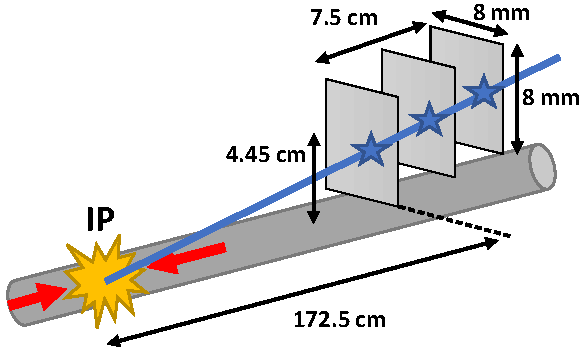
\includegraphics[width=0.5\textwidth]{images/assets/TripleCoincidenceSketch.pdf}
	\caption[Triple coincidence in PLT]{Illustration of a triple coincidence in the \acrshort{plt} detector. A hit is considered when a particle passes through the 3 sensors of a telescope (from \textit{Ref.} \cite{Lujan:2797692}).}
	\label{fig:plt_triple_coincidence}
\end{figure}

The zero-counting method, described in \autoref{subsec:zero-counting}, is used to convert the number of hits to luminosity. For PLT, the zero starvation effect is usually not a problem, as the tipical PLT occupancy is on the order 0.1-0.2 triple coincidences per telescope per bunch crossing at high luminosity conditions.

\subsection{The Fast Beam Conditions Monitor}

The \acrfull{bcm1f} \cite{CMS-DP-2022-033} can measure not only the luminosity, but also the \acrshort{bib}. It consists of 24 double-pad silicon sensors arranged in four semi-circles, referred to as ``C-shapes", positioned 7.2 cm from the beam pipe and at a distance of 1.8 m on either side of the \acrshort{ip}. This placement allows for the separation of incoming and outgoing particles, corresponding to a flight time of 6.25 ns for particles traveling at relativistic speeds. This setup enables the discernment of signals originating from collisions, \acrshort{bib}, and noise caused by the activation of surrounding material \cite{Zagozdzinska_2016}. \autoref{fig:bcm1f_real_life} shows the arrangement of one of the C-shapes.

\begin{figure}[h]
\centering
\includegraphics[width=\textwidth]{images/assets/bcm1f_real_life.png}
\caption[BCM1F sensor arrangement]{Arrangement of the six sensors in one of the C-shapes of the \acrshort{bcm1f} detector (from \textit{Ref.} \cite{DelannoySotomayor:2809025}).}
\label{fig:bcm1f_real_life}
\end{figure}

\newacronym{vme}{VME}{Versa Module Europa}
\newacronym{rhu}{RHU}{Realtime Histograming Unit}

A particle passing through the bulk of a silicon sensor will ionize the material, creating electron-hole pairs. These pairs are then separated by an electric field, generating a current pulse proportional to the energy of the particle. The signals detected in the sensors are read by two parallel systems. The older back-end system utilizes the \acrfull{vme} standard and was the primary system during Run 2. The newer $\mu$TCA-based system began operation in Run 3 \cite{Karacheban:2294183}.

The \acrshort{vme} back-end system discriminates signals using a constant threshold, and the hits are sent to a \acrfull{rhu}. The hits per bunch are then converted to luminosity using the zero-counting method. The $\mu$TCA system employs a more sophisticated approach, using a peak-finding algorithm that counts pulses based on the signal's derivative and amplitude. This method not only allows for more accurate distinction between hits and noise but also enables the detection of simultaneous hits by analyzing the pulse shape. Both systems, BCM1F and BCM1FUTCA, are used as independent luminometers.

\subsection{Pixel Cluster Counting}

A large number of modules from the \acrshort{cms} Pixel detector is also used as a luminometer. Upgraded in 2017, it consists of four barrel layers, BPIX, and three disks, FPIX, on each side of the \acrshort{ip} at distances of 291, 396, and 516 mm, respectively. The BPIX is made up of a total of 79 million pixels in 1184 modules, while the FPIX contains 45 million pixels in 672 modules. The layouts of the two detectors, the original and the upgraded one, are compared in \autoref{fig:pcc_layout}. Further details on the design and construction of the upgraded Pixel detector can be found in \cite{tracker2020cms}.

\begin{figure}[h]
\centering
\includegraphics[width=\textwidth]{images/assets/pcc_upgrade.png}
\caption[Upgraded pixel detector]{Longitudinal view of the Phase 1-upgraded pixel detector compared to the original detector layout (from \textit{Ref.} \cite{tracker2020cms}). Labels L1 to L4 indicate the barrel layers, while D1 to D3 indicate the disks.}
\label{fig:pcc_layout}
\end{figure}

The Pixel Cluster Counting (PCC) method counts the mean number of clusters, a conglomerate amount of charged particle hits, in the pixel detector in zero-bias events (events from nominally colliding bunch crossings without any specific activity requirement). The mean number of clusters, averaged over several measurements, can be expressed as

\begin{equation}
	\label{eq:pcc-clusters-mean}
	\langle N_{\text{clusters}} \rangle = \langle N_{\text{clusters} / \text{interaction}} \rangle \cdot \frac{\sigma_{\text{minBias}}}{f_{rev}} \cdot \mathcal{L}_b
\end{equation}

from which the PCC calibration factor can be calculated as $\sigma_{\text{vis}} = \sigma_{\text{minBias}} \cdot \langle N_{\text{clusters} / \text{interaction}} \rangle$ where $\sigma_{\text{minBias}}$ is the proton-proton cross section for minimum bias events. The $\langle N_{\text{clusters}} \rangle$ is measured by averaging the number of clusters over \acrshort{ls} intervals with a 0.1\% statistical uncertainty for orbit integrated luminosity.

Due the large amount of pixels used, the probability of one pixel being hit by two charged particles from the same bunch crossing is extremely small. The PCC method has been shown to provide stable and linear luminosity measurements and was used as the primary luminometer for the \acrshort{cms} experiment in previous years \cite{Sirunyan:2759951}. The measurements from this detector are only used during the offline analysis. 

\subsection{Drift Tube}
\label{subsec:dt}

Located in the \acrshort{cms} muon system, the Drift Tube (DT) is a sub-system of the muon barrel (MB) that provides an estimate of the number of muon tracks passing through the detector. This estimate, done with the Barrel Muon Track Finder (BMTF) algorithm \cite{Triossi_2017}, is assumed to be proportional to the luminosity which allows for DT to be used as a luminometer. However, it does not provide luminosity measurements with per bunch granularity, but is rather \acrshort{ls}-integrated. These limitations make the measurement of its calibration factor, $\sigma_{\text{vis}}$, dependent on the other luminometers. However, due to its good stability and linearity, it is often calibrated to match other luminometers as a way to compare for stability and linearity.

%%%%%%%%%%%%%%%%%%%%%%%%%%%%%%%%%%%%%%%%%%%%%%%%%%%%%%%%%%%%%%%%%
%% LUMINOMENTER: TO APPROACH AFTER KNOWING WHAT LUMINOISITY IS %%
%%%%%%%%%%%%%%%%%%%%%%%%%%%%%%%%%%%%%%%%%%%%%%%%%%%%%%%%%%%%%%%%%

\chapter{Luminosity Calibration at the LHC}

CERN’s mission of understanding the fundamental structure of the universe is heavily reliant on particle accelerators. The effectiveness of the experiments conducted in these machines is closely tied to their luminosity, as detailed in \autoref{sec:luminosity}. 
In this chapter, the van der Meer (vdM) scan methodology used to measure the luminometer's calibration factor is explained first. Subsequently, the corrective procedures applied to optimize the accuracy and precision of this method are discussed. Finally, the challenges associated with extrapolating the results obtained with the vdM method for the rest of the data-taking period are addressed.
\section{Absolute luminosity calibration}
\label{sec:absolute_luminosity_calibration}

As explained in \autoref{subsec:luminosity_calibration}, all luminometers require a specific calibration, $\sigma_{vis}$, to convert their measured rates into an absolute measurement of luminosity. A common limitation in making precise theoretical predictions of Standard Model processes is the uncertainty in the parton distribution functions within the proton \cite{GRAFSTROM201597. These limitations necessitate methods that do not rely on theoretical assumptions of these distributions. While data-driven methods have been proposed, they introduce correlations between low and high pileup data-taking periods \cite{Salfeld-Nebgen_2018}. A more precise and purely experimental procedure to determine this detector calibration is the van der Meer (vdM) scan methodology.

In order to measure the visible cross-section, beam scans are performed, in which the two LHC beams are moved with respect to each other in the transverse ($x-y$) plane in incremental steps. This procedure was pioneered by Simon van der Meer at the Intersecting Storage Rings (ISR) \cite{vanderMeer:296752} and extend by Carlo Rubbia to the case of a collider with bunched beams \cite{Rubbia:1025746}. Instead of measuring the transverse bunch density functions, this method allows for the measurement of the bunch overlap integral from the rates measured at different beam separations. This method has been used by every LHC experiment \cite{TheLHCbcollaboration_2014, ALICE-PUBLIC-2021-001, Maettig:1513982, Sirunyan:2759951}.

\subsection{The van der Meer Scan Methodology}
\label{subsec:the_van_der_meer_scan_methodology}

Recalling \autoref{eq:sbil-machine-params} and \autoref{eq:effective-area}, we can rewrite the SBIL expression for beams separated by $\Delta_x$ in the horizontal plane and $\Delta_y$ in the vertical plane as:

\begin{equation}
    \label{eq:sbil_separating_planes}
    \mathcal{L}_b \left( \Delta_x, \Delta_y \right) = N_1 N_2 f_{rev} \int \rho_1 (x, y) \rho_2 (x + \Delta_x, y + \Delta_y) dx dy
\end{equation}

As shown in \cite{vanderMeer:296752}, when a separation scan is performed in either transverse direction, where $\Delta_x$ and/or $\Delta_y$ is varied in a step-wise manner, the effective width and height of the luminous region can be expressed as:

\begin{equation}
    \begin{aligned}
        \label{eq:effective_width_height_scan}
        W_{eff} = \frac{\int \int \rho_1 (x) \rho_2 (x + \Delta_x) dx d\Delta_x}{\int \rho_1 (x) \rho_2 (x) dx} = \frac{\int \mathcal{L}_b \left( \Delta_x, 0 \right) d\Delta_x}{\mathcal{L}_b \left( 0, 0 \right)} \\
        H_{eff} = \frac{\int \int \rho_1 (y) \rho_2 (y + \Delta_y) dy d\Delta_y}{\int \rho_1 (y) \rho_2 (y) dy} = \frac{\int \mathcal{L}_b \left( 0, \Delta_y \right) d\Delta_y}{\mathcal{L}_b \left( 0, 0 \right)}
    \end{aligned}
\end{equation}

where the beam populations, $N_1$ and $N_2$, and the LHC revolution frequency have been canceled in the second step for both equations.

Assuming Gaussian-distributed bunches, the scan curves $\mathcal{L}_b \left( \Delta_x, 0 \right)$ and $\mathcal{L}_b \left( 0, \Delta_y \right)$ will also be Gaussian. Thus, we arrive at the equality expressed in \autoref{subsec:luminosity_from_machine_parameters}, where $\Sigma_X = \sqrt{2\pi} W_{eff}$ and $\Sigma_Y = \sqrt{2\pi} H_{eff}$, thereby proving the equivalence of the method. However, as mentioned at the beginning of this section, no assumptions are made about the nature of the particle bunch distribution, which means the scan curves are not guaranteed to be Gaussian.

Frequently, these curves are not well described by simple Gaussians. In this analysis, we fit these curves with Double Gaussian (DG) functions of the form:

\begin{equation}
    f_{\text{DG}}(\chi) = 
    \frac{r_{\chi}}{\sqrt{2\pi}} 
    \left[ 
        \frac{\epsilon_{\chi}}{\sigma_{1_{\chi}}} \text{exp} \left( -\frac{\left( \Delta_{\chi} - \mu_{\chi} \right)^2}{2\sigma^2_{1_{\chi}}} \right) +
        \frac{1 - \epsilon_{\chi}}{\sigma_{2_{\chi}}} \text{exp} \left( -\frac{\left( \Delta_{\chi} - \mu_{\chi} \right)^2}{2\sigma^2_{2_{\chi}}} \right)
    \right]
    \label{eq:double_gaussian_model}
\end{equation}

where $\chi \in \{X, Y\}$ denotes the scanning plane, $\Delta_{\chi}$ is the nominal beam separation, $r_{\chi}$ and $\mu_{\chi}$ are the peak and peak position of the DG and $\sigma_{1_{\chi}}$, $\sigma_{2_{\chi}}$ are the widths of the two individual Gaussians. The two gaussians are weighted by $\epsilon_{\chi}$ and $1 - \epsilon_{\chi}$, respectively, and $\Sigma_{X}$ and $\Sigma_{Y}$ are related to the individual beam widths by: 

\begin{equation}
    \Sigma_{\chi} = \frac{\sigma_{1_{\chi}}\sigma_{2_{\chi}}}{\epsilon_{\chi}\sigma_{2_{\chi}} + \left( 1 - \epsilon_{\chi}\right) \sigma_{1_{\chi}}}
\end{equation}

The visible cross-section, $\sigma_{vis}$, can also be expressed as a function of the fit parameters as:

\begin{equation}
    \sigma_{\mathrm{vis}} =  \frac{2\pi \Sigma_{X} \Sigma_{Y} R_{peak}}{N_1 N_2 f_{rev}}
    \label{eq:calibration_from_fit_parameters}
\end{equation}

where $R_{peak}$ is taken as the arithmetic mean of the peak values, $r_X$ and $r_Y$, of both scan curves. This fit procedure is applied for every bunch crossing. Since the cross-section results heavily dependent on how well the fit converges we only apply this method on the luminometers which have per-bunch granularity.

\autoref{fig:vdm_scan_steps} ilustrates the beam separations during two vdM scans, one in each transverse direction.

\begin{figure}[!htb]
	\centering
	\includegraphics[width=\textwidth]{images/assets/vdm_scan_steps.png}
	\caption[Example vdM scan sequence positions]{Nominal LHC beam positions displaying the van der Meer scan sequence first in $x$-axis and then in $y$-axis (from \textit{Ref.} \cite{Saariokari:2826125}).}
	\label{fig:vdm_scan_steps}
\end{figure}

\subsection{Experimental Conditions and Corrective Procedures}
\label{sec:experiment_conditions_and_corrective_procedures}

A vdM scan is conducted under experimental conditions that allow for the measurement of the visible cross-section to the highest precision. These conditions include smaller beam intensities, which minimize the effect of \acrshort{bib} and reduce non-linearity effects, and well-separated bunches, which minimize afterglow effects \cite{GRAFSTROM201597}. In addition to these optimized experimental conditions, a series of offline corrections are performed to ensure the required level of precision. These corrections include:

\begin{itemize}
    \item \textbf{Background estimation:} Background signals, whether beam-induced, from detector noise, or machine-induced, are typically present in the raw recorded rates. These additional contributions are removed.
    \item \textbf{Beam current measurement:} Various systems measure and monitor the beam conditions throughout the entire fill to enable offline corrections, such as the removal of spurious charges.
    \item \textbf{Beam-beam effects:} The electromagnetic interaction between the two LHC beams causes disturbances in the nominal beam separation and shapes, affecting the calibration measurement \cite{Babaev2024}. These effects are accounted for and corrected in the analysis.
    \item \textbf{Orbit drift:} During the vdM fill, the nominal position of the LHC beams may shift. These shifts are measured by Beam Position Monitors (BPM), which provide information to correct the nominal beam separations.
    \item \textbf{Length scale calibration:} The operational displacement of the LHC beams is achieved using a pair of steering dipoles located on either side of the IP. These displacements come with associated uncertainties due to effects such as magnet hysteresis or lattice imperfections \cite{Persson:2750277}. These effects are taken into account.
    \item \textbf{XY factorization:} The vdM method assumes that the transverse particle distributions are independent in each tranverse direction and therefore factorizable. If this assumption is not true, the calculated value for \(A_{eff}\) will be biased. Studies are conducted to understand the magnitude of this bias and correct it.
\end{itemize}

A more detailed explanation of these corrections, as well as their impact on the measured calibration, will be provided in \autoref{ch:2023_luminosity_calibration}.

\subsection{Extrapolation of vdM Calibration}
\label{subsec:extrapolation_of_vdM_calibration}

The experimental conditions in which a vdM fill is performed, as well as all the extra corrections applied to the collected data, ensure a cross-section measurement with high precision and accuracy. However, the optimal experimental conditions for probing the Standard Model, known as ``physics conditions", introduce several effects that impact the calibration of the luminometers. Therefore, it is necessary to extrapolate the results obtained during a vdM fill to correctly calibrate the luminosity measured under physics conditions.

Physics conditions are tailored to obtaining the largest amount of data possible. This includes higher bunch populations compared to vdM fills and more colliding bunches, all of which increase the number of colliding particles. These conditions bring about two classes of effects on our luminometers:

\begin{itemize}
    \item \textbf{Efficiency effects:} Prolonged exposure to ionizing radiation from highly-energetic interactions deteriorates the luminometers, making them less efficient. These effects result in a gradual decrease in the reported luminosity throughout the data-taking period.
    \item \textbf{Non-linearity effects:} Varying experimental conditions can affect the reported luminosity of our detectors, as mentioned in \autoref{subsec:luminosity_detectors}. While some of these effects have their own corrective procedures, such as out-of-time pileup \cite{Sirunyan:2759951}, others are corrected empirically.
\end{itemize}

To account for these two classes of effects, the measured luminosity undergoes a final correction described by \autoref{eq:luminosity_integration}.

\begin{equation}
    \centering
    \mathcal{L} = \frac{f_{rev} \cdot \mu}{\sigma_{vis} \cdot \epsilon} - \alpha \left( \frac{f_{rev} \cdot \mu}{\sigma_{vis} \cdot \epsilon} \right)^{2}
    \label{eq:luminosity_integration}
\end{equation}

Two new parameters have been introduced. \(\epsilon\) is the parameter that corrects for losses in detector efficiency throughout the data-taking period. To obtain these factors, mini vdM-like scans, called emittance scans (em), are performed. These scans are used to measure the visible cross-section using the same vdM method, allowing for the analysis of the evolution of this quantity over the data-taking period. A figure of merit (FOM) is then calculated as:

\begin{equation}
    \centering
    \text{FOM} = \frac{\sigma^{\text{vdM}}_{vis}}{\sigma^{\text{emit}}_{vis}}
    \label{eq:figure_of_merit}
\end{equation}

where \(\sigma^{\text{vdM}}_{vis}\) is the visible cross-section measured under vdM conditions, and \(\sigma^{\text{emit}}_{vis}\) is the visible cross-section measured during emittance scans under physics conditions. These FOM values are calculated for every emittance scan throughout the data-taking period and used to correct for variations in each luminometer's efficiency.

The second new parameter, \(\alpha\), corrects for any non-linearity in the luminometers and is derived empirically. Non-linearity is defined as any non-linear response to changes in experimental conditions. \autoref{fig:non_linearity_diagram} illustrates the response of a theoretical linear detector, a detector with positive non-linearity, and a detector with negative non-linearity.

\begin{figure}[!htb]
    \centering
    \makebox[\textwidth]{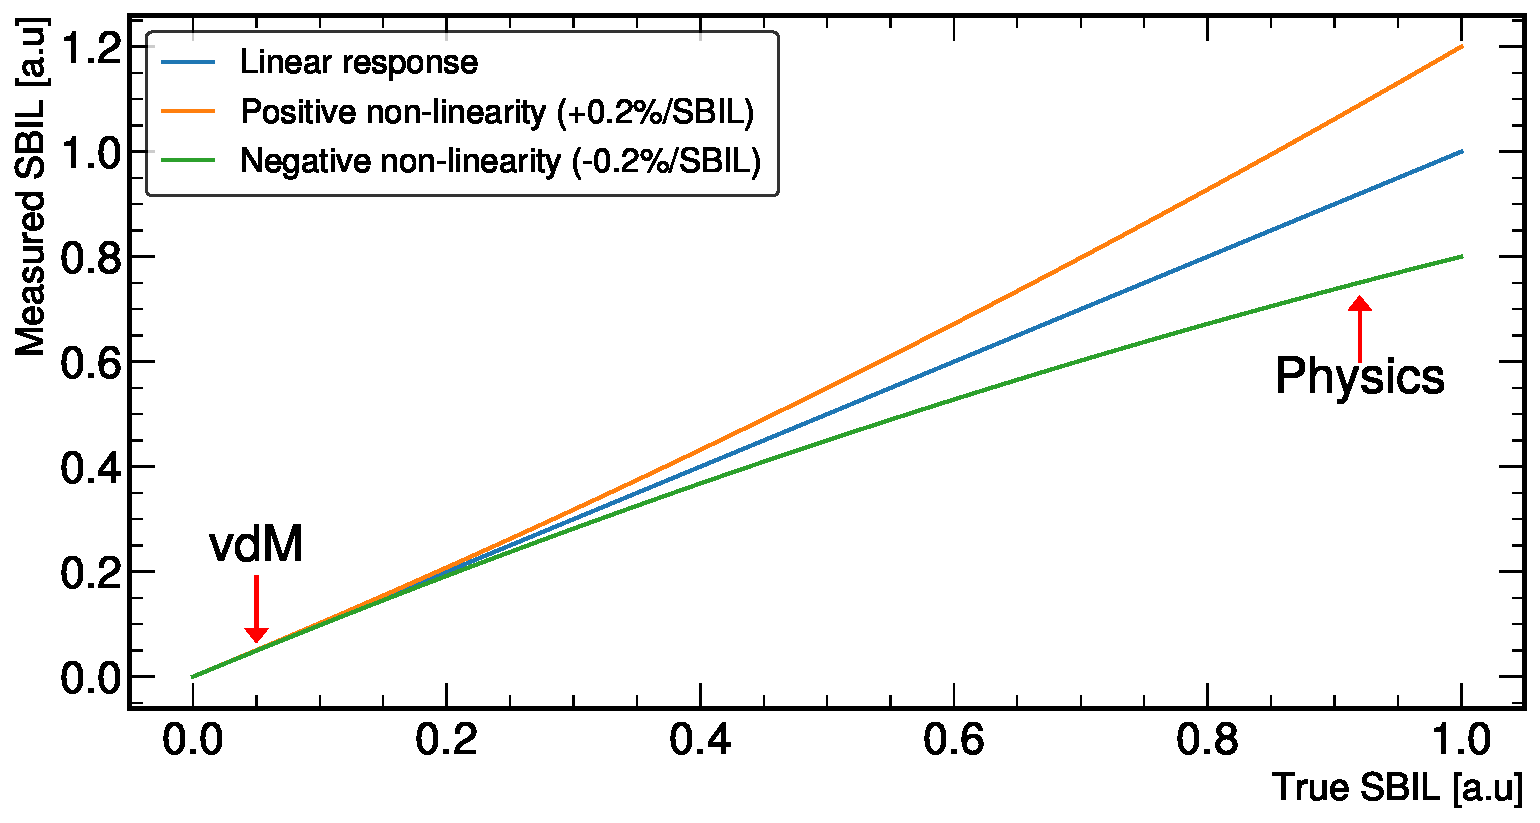
\includegraphics[width=0.7\paperwidth]{images/assets/non_linearity_diagram.pdf}}
    \caption[Non-linearity effects on SBIL]{Illustration of non-linearity effects on measured SBIL as a function of the true SBIL. The two marked regions illustrate the effects of extrapolating from vdM to physics conditions.}
    \label{fig:non_linearity_diagram}
\end{figure}

The reasons for a detector to have a positive or negative non-linear response vary:

\begin{itemize}
    \item PLT has consistently shown signs of positive non-linearity, mainly due to the increased probability of ``accidental" triple coincidences at higher pileup due to background tracks, leading to overcounting.
    \item HFOC suffers from the ``zero starvation" effect, as explained in \autoref{subsec:zero-counting}, leading to an underestimation of the measured rates, categorized as negative non-linearity.
\end{itemize}

Correcting for non-linearity is challenging due to the lack of a perfectly linear reference detector. Instead, a reference detector, assumed to be linear, is used. In this method, a linear fit is performed on the ratio between a luminometer and this reference detector as a function of SBIL. 

The slope extracted from the fit is then used as the value of \(\alpha\) in \autoref{eq:luminosity_integration}. Unlike the efficiency corrections (\(\epsilon\)), the non-linearity corrections are done at the expense of introducing some degree of correlation between the corrected detector and the reference. To keep the luminometers as independent as possible, the slopes are extracted for only a few fills with a high SBIL range throughout the year.

The specialized vdM conditions, along with the series of corrections applied to the vdM data and the extrapolation to physics conditions, all contribute to the significant challenge of accurately measuring luminosity at hadron colliders like the LHC.

\subsection{Additional Scans}

In addition to the vdM scan, other types of scans are performed during the vdM fill to provide specific insights into the various experimental conditions:

\begin{itemize}
    \item \textbf{Super Separation scans (ss):} These scans involve maximally separating the beams in the LHC, allowing for an accurate measurement of the background for each luminometer.
    \item \textbf{Beam Imaging scans (im):} In these scans, one beam is kept fixed in its nominal head-on position while the other beam is scanned. These scans are used for the beam-imaging method \cite{Klute_2017}, which is employed in XY factorization analysis. A visible cross-section is also extracted from these scans, similar to vdM scans.
    \item \textbf{Diagonal scans (diag):} These are vdM scans performed at distinct angles, such as +45º/-45º, +30º/-60º, and +60º/-30º. They allow the fitting to occur over different regions of the beam overlap and are used in XY factorization studies.
    \item \textbf{Offset scans (off):} These scans have the same motion as vdM scans, but one of the beams is not in the nominal head-on position. They are used in beam shape studies to determine the XY factorization bias.
    \item \textbf{Variable/Constant length scale scans (vls, cls):} These scans involve moving the beams together at constant or variable separation and are used to calibrate the distance by which the steering magnets displace the beams.
\end{itemize}

Each scan is separately recorded and analyzed offline. After thorough analysis, the corrective procedures determined from each of these special scans are applied to the vdM scan analysis to correct the extracted detector calibration. In principle, these corrections affect every luminometer in a similar fashion.

\input{chapters/ProblemAndChallenges}

\chapter{2023 Luminosity Calibration}
\label{ch:2023_luminosity_calibration}

\section{Analysis of vdM data}

CMS's vdM scan program was performed in June 2023 during LHC fill 8999. During this fill, there were 138 filled bunches per beam and a total of 136 colliding bunches at the CMS IP. The bunches were designed to be wider than usual ($\beta^{*} = 1920 cm$) and separated by $525 ns$ in order to minimize afterglow effects. In order to minimize non-linear effects, the pileup was significantly limited from the average during 2023, $52$, to just $0.5$.

The LHC beam positions throughout the entire vdM program is shown in \autoref{fig:vdm_fill_program}.

\begin{figure}[!htb]
	\centering
	\makebox[\textwidth]{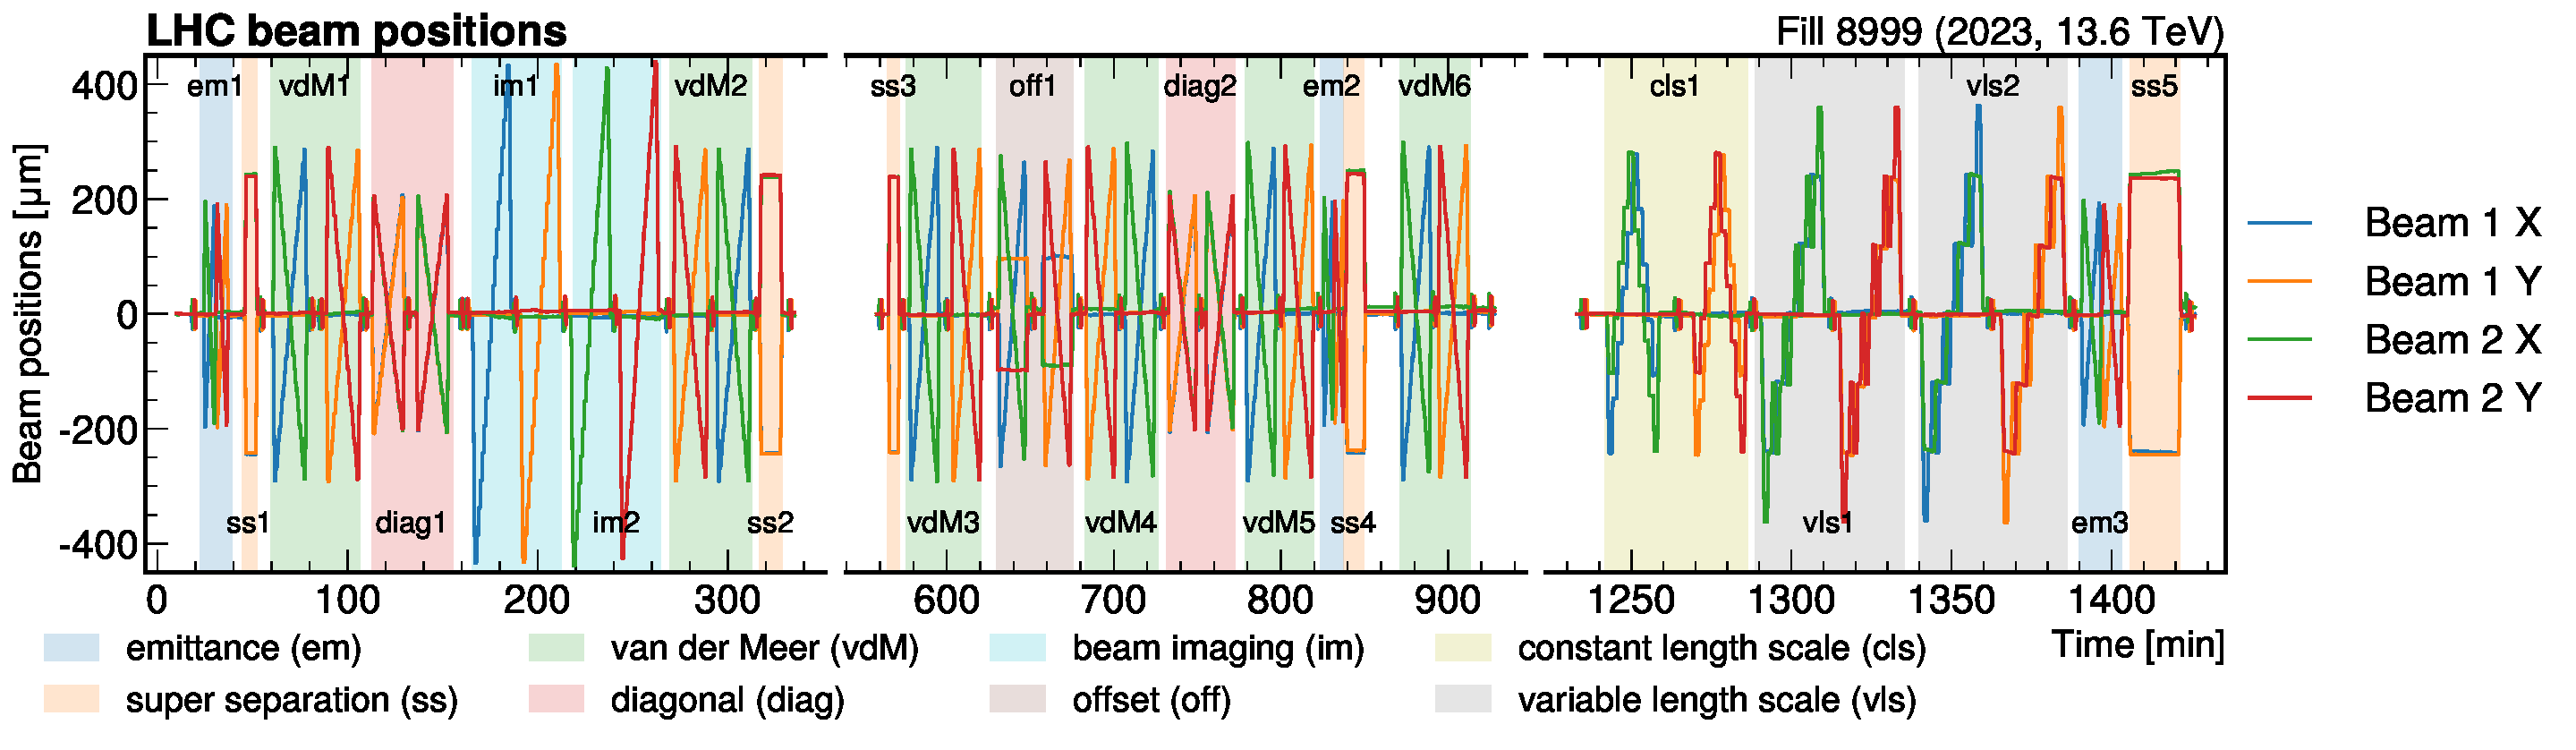
\includegraphics[width=0.95\paperwidth]{images/assets/vdm_fill_program.pdf}}
	\caption[Beam positions during fill 8999]{The vertical (X) and horizontal (Y) positions of beam 1 and beam 2 are shown as a function of time during LHC fill 8999 as measured by the LHC beam position monitors. Each kind of scan pair, which contains two orthogonal scans, is delimited by the shaded regions and labeled with the appropriate scan name. The cut out time periods correspond to when CMS was taking head-on data while the ATLAS vdM scan program was ongoing.}
	\label{fig:vdm_fill_program}
\end{figure}

As can be seen in \autoref{fig:vdm_fill_program}, during the vdM scans, the beams start by being maximally separated by approximately $578 \mu m$. They are then scanned across each other in 25 steps of approximately $48 \mu m$, remaining in the same position for 30 seconds for each step. In the beam imaging scans, one of the beams is fixed in the nominal head-on position while the other is moved from approximately $-433 \mu m$ to $+433 \mu m$ in 19 steps of 46 seconds each.

The measured luminometer rates are fitted as a function of the beam separation with the model described in \autoref{eq:double_gaussian_model} and the luminometer calibrations are determined from the fit parameters as detailed in \autoref{eq:calibration_from_fit_parameters}. The fits were performed on the data from the 6 vdM and the 2 im scan pairs and its associated visible cross sections were measured. \autoref{fig:no_Corr_xsec_results_HFET} shows the visible cross section measurement results for the HFET luminometer with none of the corrections mentioned in \autoref{sec:experiment_conditions_and_corrective_procedures} having been applied.

\begin{figure}[!htb]
	\centering
	\makebox[\textwidth]{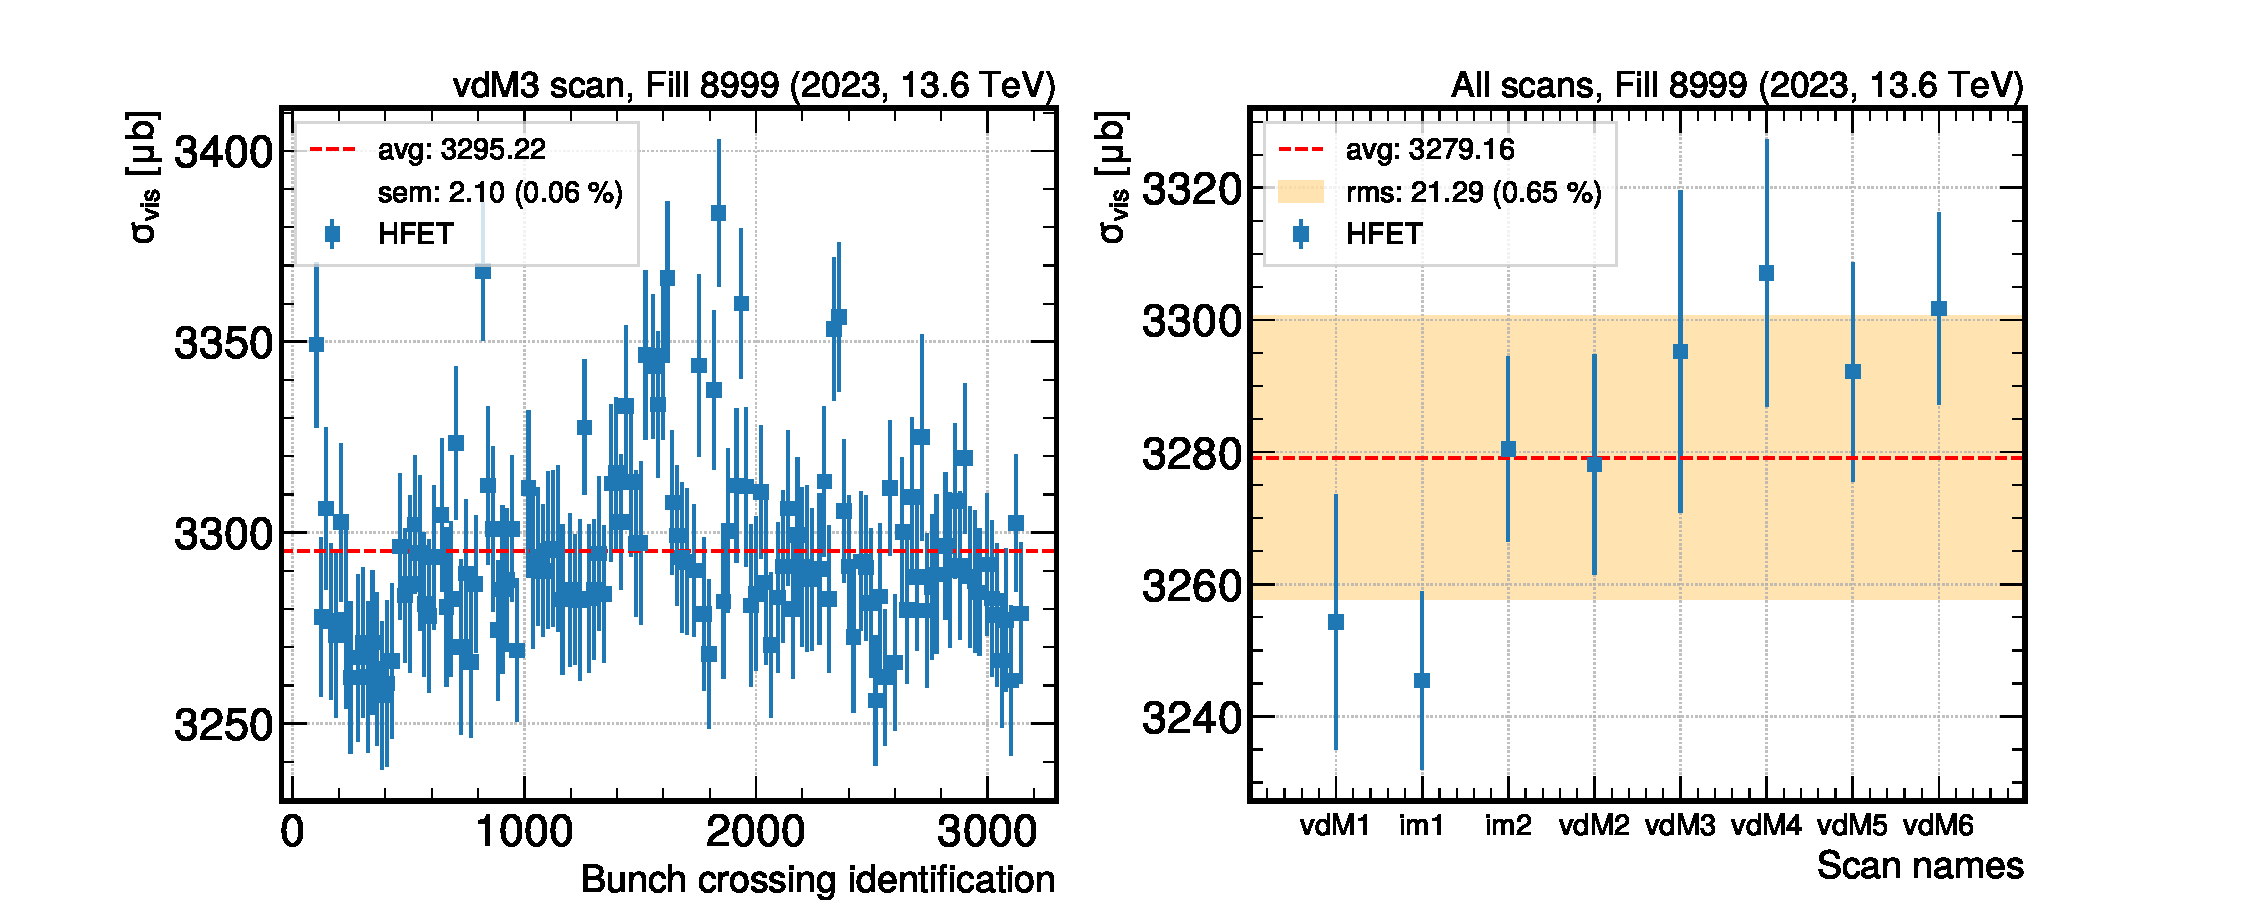
\includegraphics[width=0.9\paperwidth]{images/assets/no_Corr_xsec_results_HFET.pdf}}
	\caption[Initial HFET visible cross section results]{Initial visible cross section results obtained from uncorrected, raw data for the HFET luminometer, as an example. On the left, the measured per-bunch visible cross sections with their associated fit uncertainties are shown. The standard error on the mean (sem) is also depicted in the legend. The right image shows the measured visible cross section taking the average over all 136 BCIDs for each vdM and im scan pairs. The error bars are defined by the root mean squared (RMS) over all BCIDs. The central value and its uncertainty are determined by calculating the uncertainty-weighted average and  standard deviation over the scan pairs.}
	\label{fig:no_Corr_xsec_results_HFET}
\end{figure}

There is a noticeable increasing trend in the measured visible cross sections as a function of time. Furthermore, this trend is visible in all other luminometers, as can be seen in \autoref{fig:noCorr_luminometer_xsec}.

\begin{figure}[!htb]
	\centering
	\makebox[\textwidth]{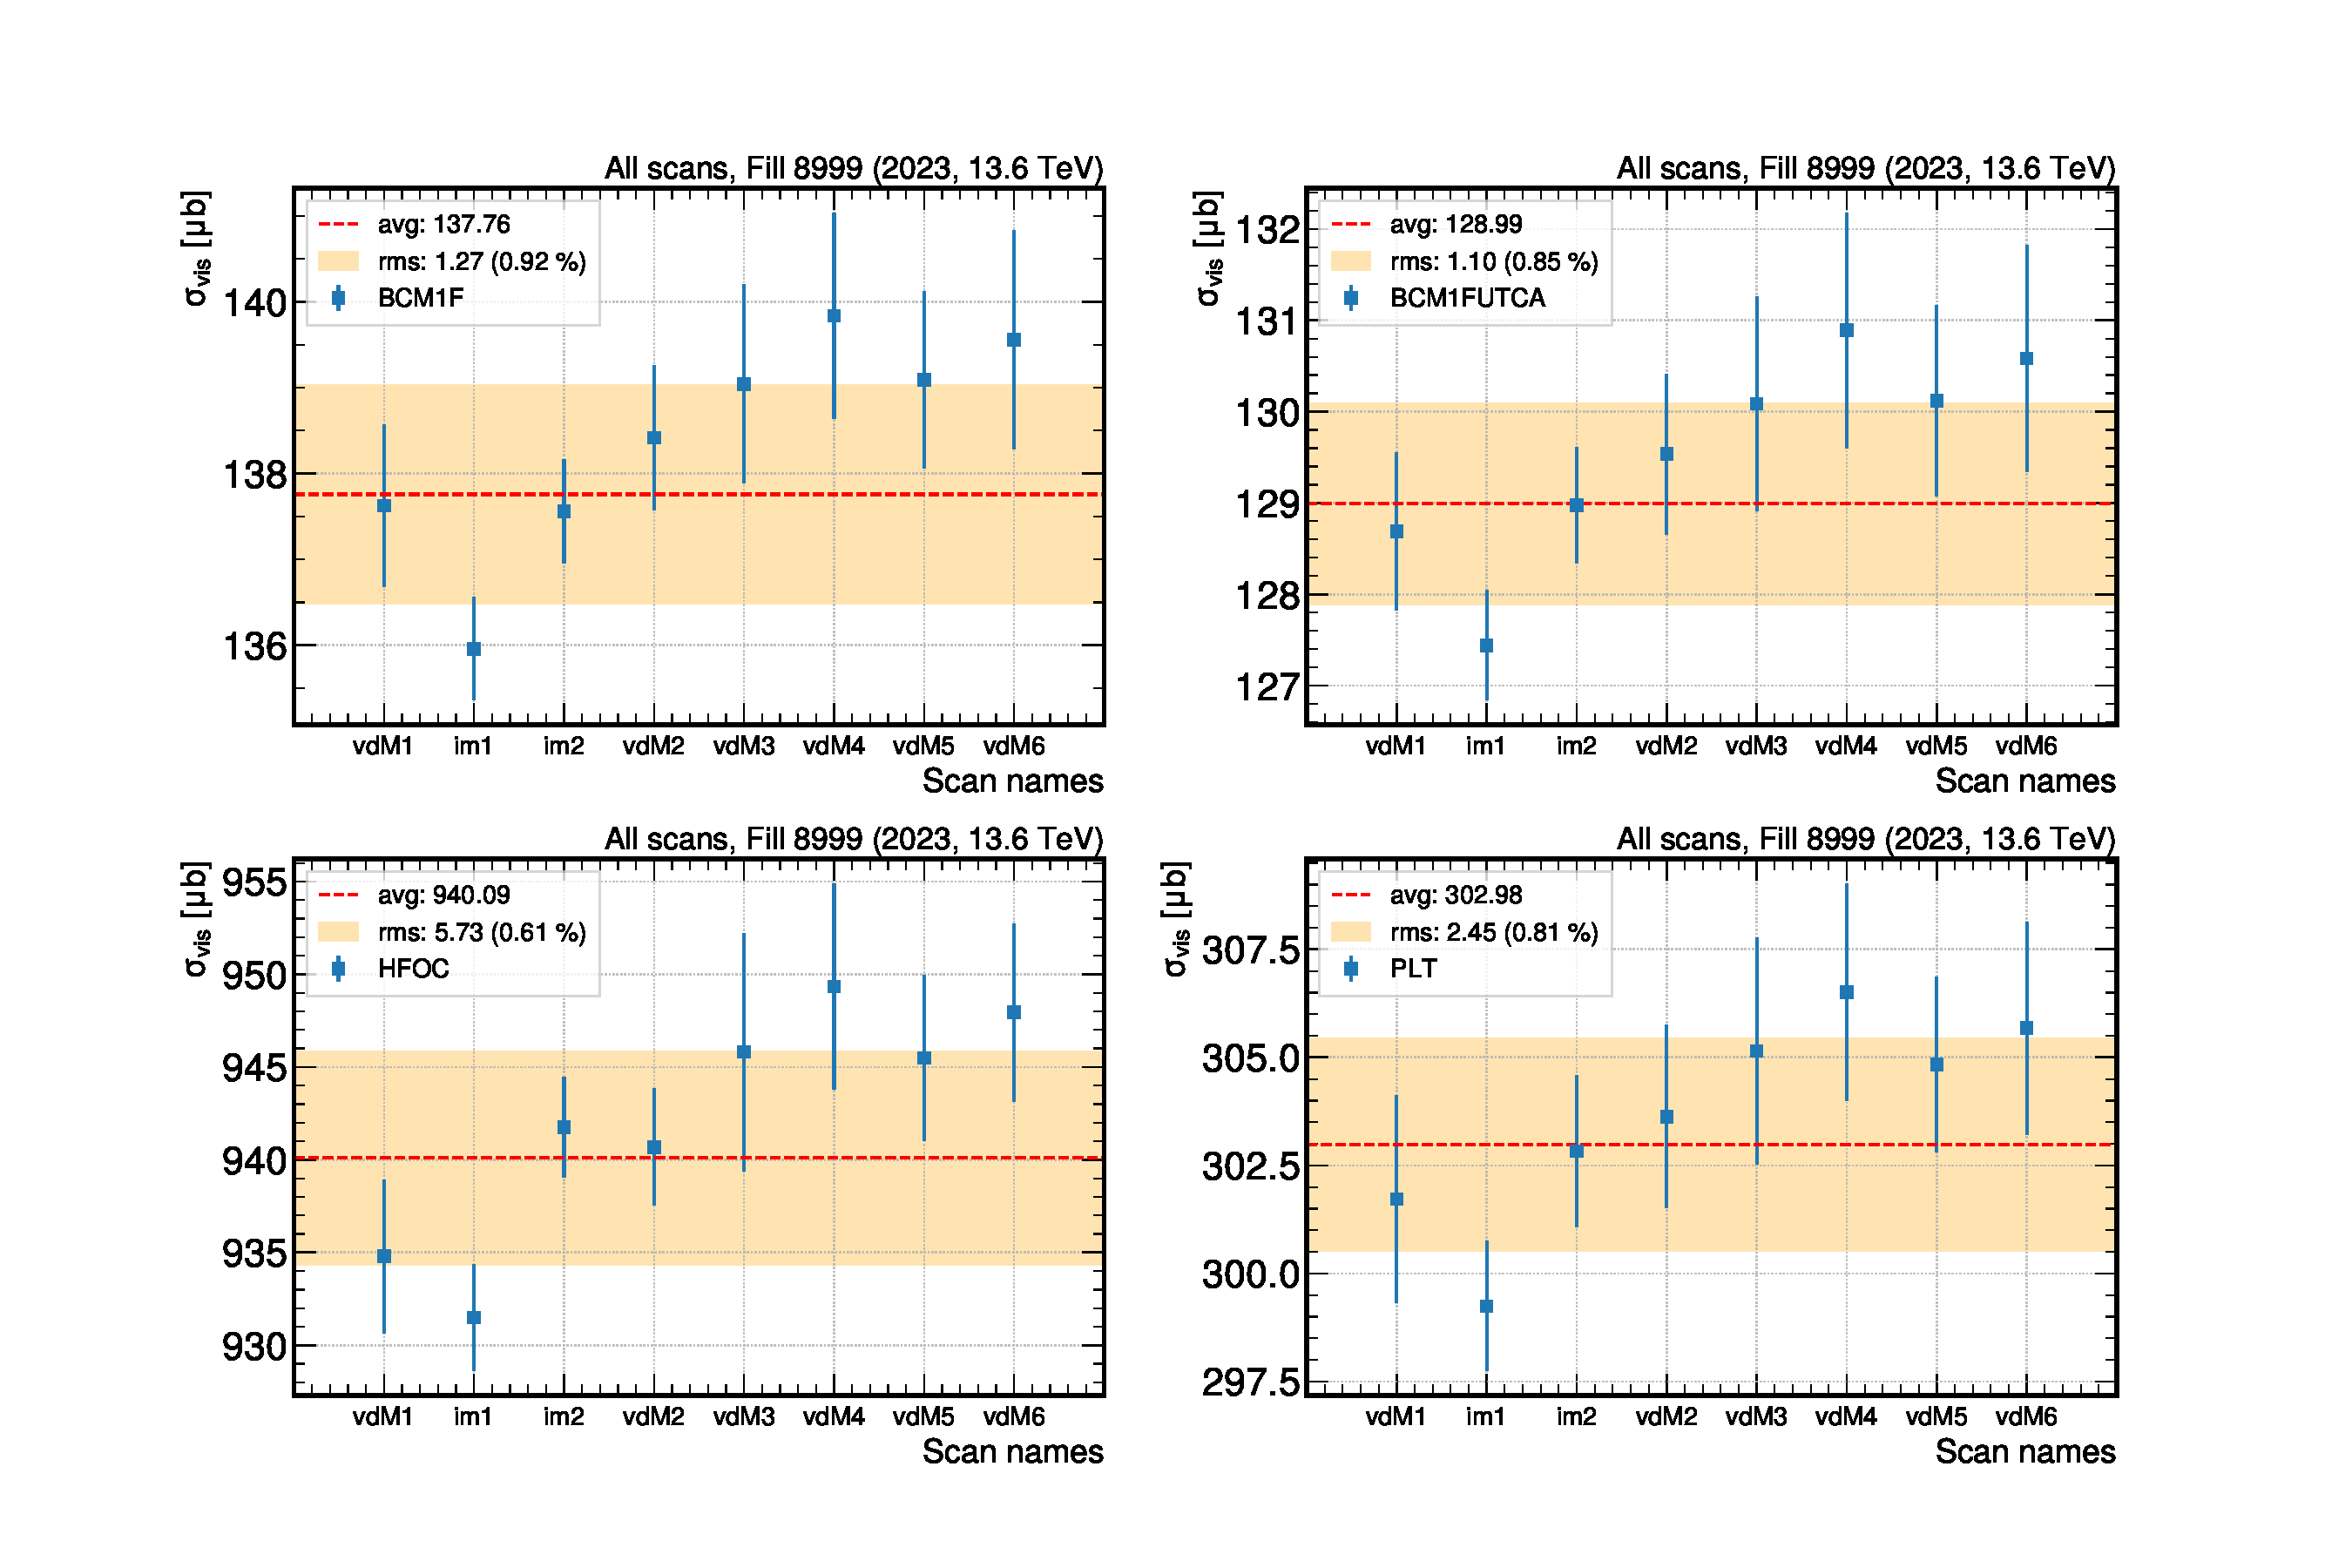
\includegraphics[width=0.9\paperwidth]{images/assets/noCorr_luminometer_xsec.pdf}}
	\caption[Initial visible cross section for other online luminometers]{Initial visible cross section results obtained from uncorrected, raw data for BCM1F, BCM1FUTCA, HFOC and PLT luminometers.}
	\label{fig:noCorr_luminometer_xsec}
\end{figure}

To increase the precision and accuracy of these measurements, a series of corrections have been applied to the raw data as will be described in the next subsections.

\subsection{Background estimation}

Beam-induced background and detector noise are both sources of background that are taken into account and subtracted from the raw detector rates. These sources have been estimated via two distinct methods:

\begin{itemize}
	\item \textbf{Estimation from super-separation scans}: The background contribution can be directly measured from super-separation scans (denoted as ss in \autoref{fig:vdm_fill_program}). During these scans, the beams are separated in both planes in order to render the contributions from collision products negligible. This method is most commonly used during special fills, such as the vdM fill, since it consumes beam time.
	\item \textbf{Estimation from non-colliding bunches}: An estimation for background can be done as long as there are filled but non-colliding bunches in the filling scheme. This indirect method assumes the background in colliding bunches can be described as:
	\begin{equation}
		\label{eq:bkg_eq1}
		\mathrm{BKG} = 2 \cdot \mathrm{BIB} + \eta
	\end{equation}
	where the beam-induced background, $\mathrm{BIB}$, from the two beams is considered as well as the detector-specific noise, $\eta$. Furthermore, $\mathrm{BIB}$ is calculated like:
	\begin{equation}
		\label{eq:bkg_eq2}
		\mathrm{BIB} = \mathrm{FNCR} + \eta.
	\end{equation}
	Here, $\mathrm{FNCR}$, is the measured rate from filled non-colliding bunches. Finally, the detector noise is calculated as the average signal from empty non-colliding bunches, $\mathrm{ENCR}$. Combining \autoref{eq:bkg_eq1} and \autoref{eq:bkg_eq2}, the background in colliding bunches is calculated as:
	\begin{equation}
		\mathrm{BKG} = 2 \cdot \mathrm{FNCR} + \mathrm{ENCR}.
	\end{equation}
    This method heavily relies on the number of filled non-colliding bunches, of which there were only two in the vdM fill, in order to accurately measure $\mathrm{BIB}$. Since super separation scans are never done under physics conditions, this method is the only option available for emittance scans during physics fills.
\end{itemize}

\autoref{fig:8999SuperSeparation_BCM1FUTCA} shows the BCM1FUTCA average of the measured rates for every BCID using the super-separation scan method. \autoref{tab:ss_summary} summarizes the measured background contributions for all the luminometers except for HFET since its background subtraction is applied online.

\begin{figure}[!htb]
	\centering
	\makebox[\textwidth]{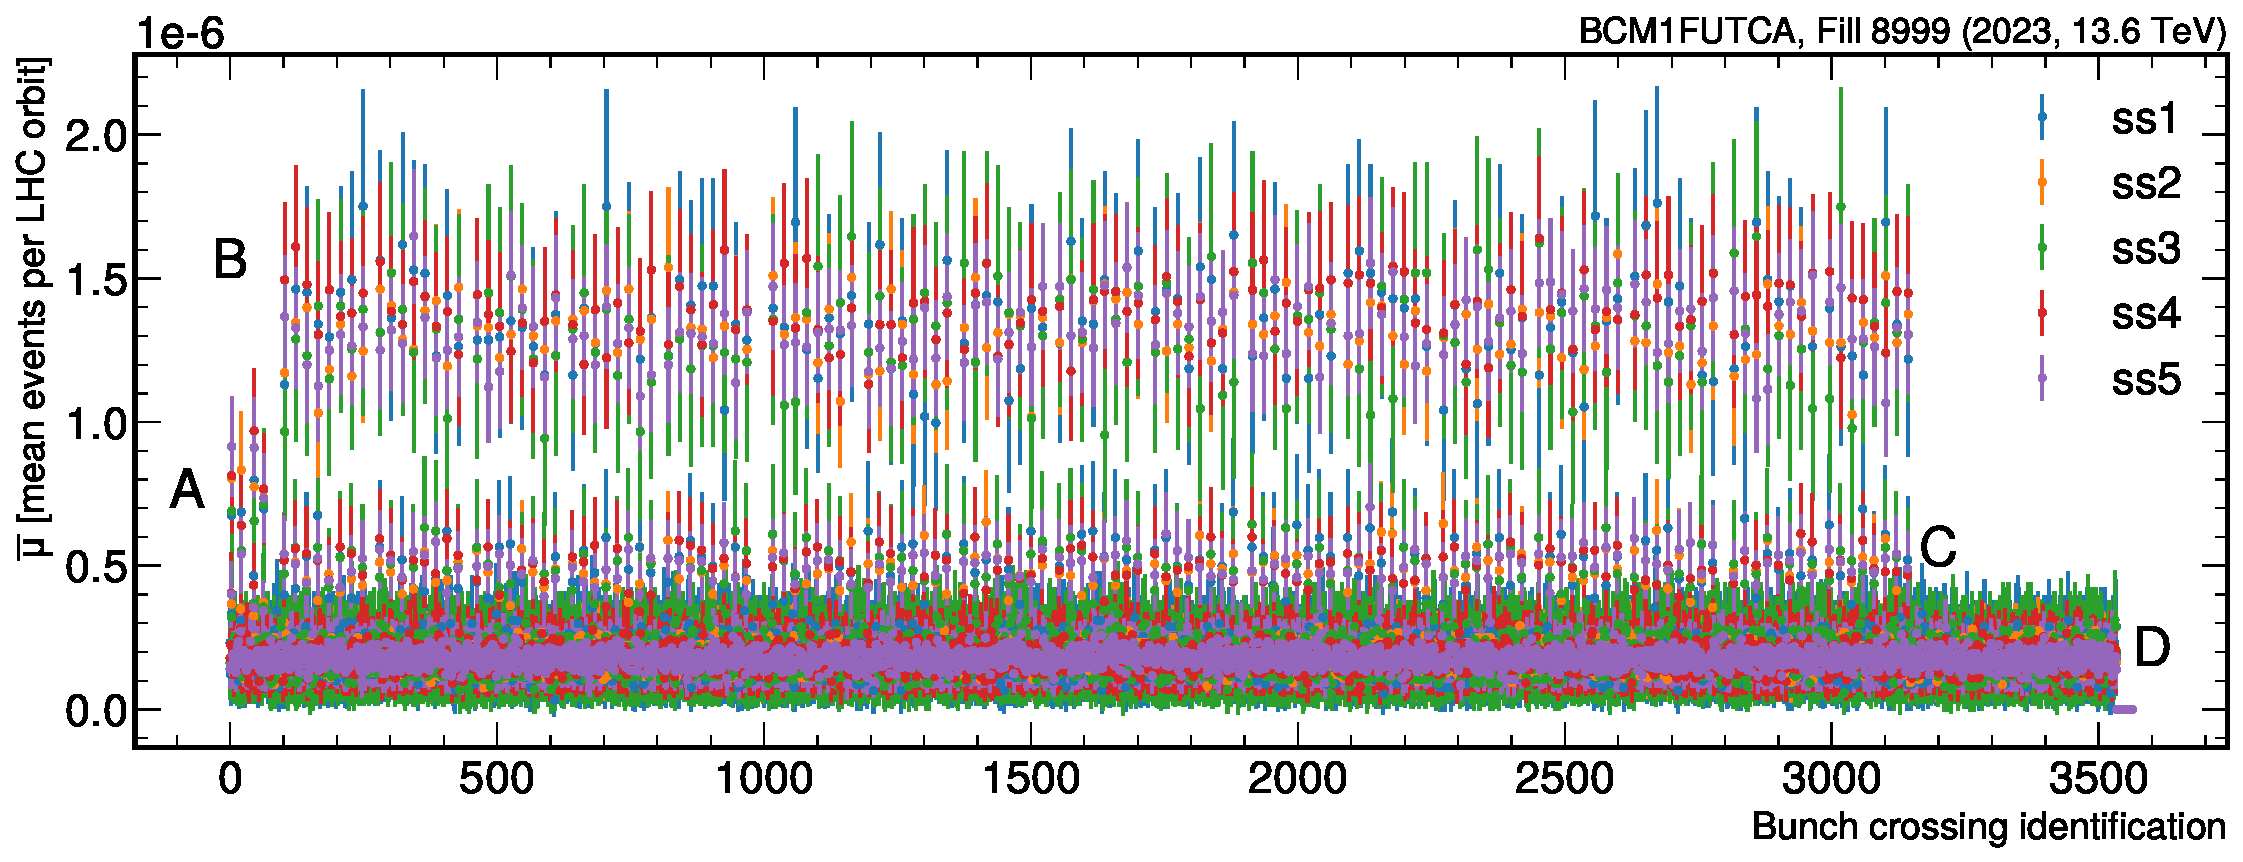
\includegraphics[width=0.8\paperwidth]{images/assets/8999SuperSeparation_BCM1FUTCA.pdf}}
	\caption[BCM1FUTCA hits in super-separation scan]{BCM1FUTCA average of the measured rates per BCID during super separation scans. The labels A, B, C, and D refer to the following: A represents the four filled non-colliding BCIDs at the beginning of the orbit, B represents the 136 colliding BCIDs (indicated by the top band), C corresponds to the empty BCIDs adjacent to filled BCIDs (around 0.5), and D represents the remaining empty non-colliding bunches.}
	\label{fig:8999SuperSeparation_BCM1FUTCA}
\end{figure}

\begin{table}[!htb]
	\centering
	\caption[Background impact on calibration]{Summary of measured background per luminometer and its impact on the vdM calibration. The average is computed on the measured background for all the colliding bunches across all scans. The associated uncertainty is the standard error on the average.}
	\begin{tabular}{lcccc}
		\hline
		Luminometer & Average [$\overline{\mu}$] & Uncertainty [$\overline{\mu}$] & \% to peak rate at vdM1 & Effect on $\sigma_{\mathrm{vis}}$ (\%) \\
		\hline
		BCM1F & 1.59E-6 & 4.68E-9 & 0.18 & -1.56 \\
		BCM1FUTCA & 1.34E-6 & 4.63E-9 & 0.16 & -1.39 \\
		HFOC & 1.17E-7 & 6.10E-9 & 0.002 & -0.02 \\
		PLT & 2.11E-6 & 9.25E-9 & 0.11 & -1.05 \\
		PCC & 1.65E-2 & 6E-4 & 0.12 & -1.08 \\
		\hline
	\end{tabular}
	\label{tab:ss_summary}
\end{table}

\subsection{Beam current measurement}
\label{subsec:beam_current_measurement}

The beam currents play a crucial role in the determination of the visible cross section, serving as a normalization factor to the detector rates, as can be seen from \autoref{eq:calibration_from_fit_parameters}. In the LHC, they are measured with two dedicated instruments: the Fast Beam Current Transformer (FBCT) \cite{Belohrad:1267400} and the Direct-Current Current Transformer (DCCT) \cite{Odier:1183400}.

\begin{figure}[!htb]
	\centering
	\makebox[\textwidth]{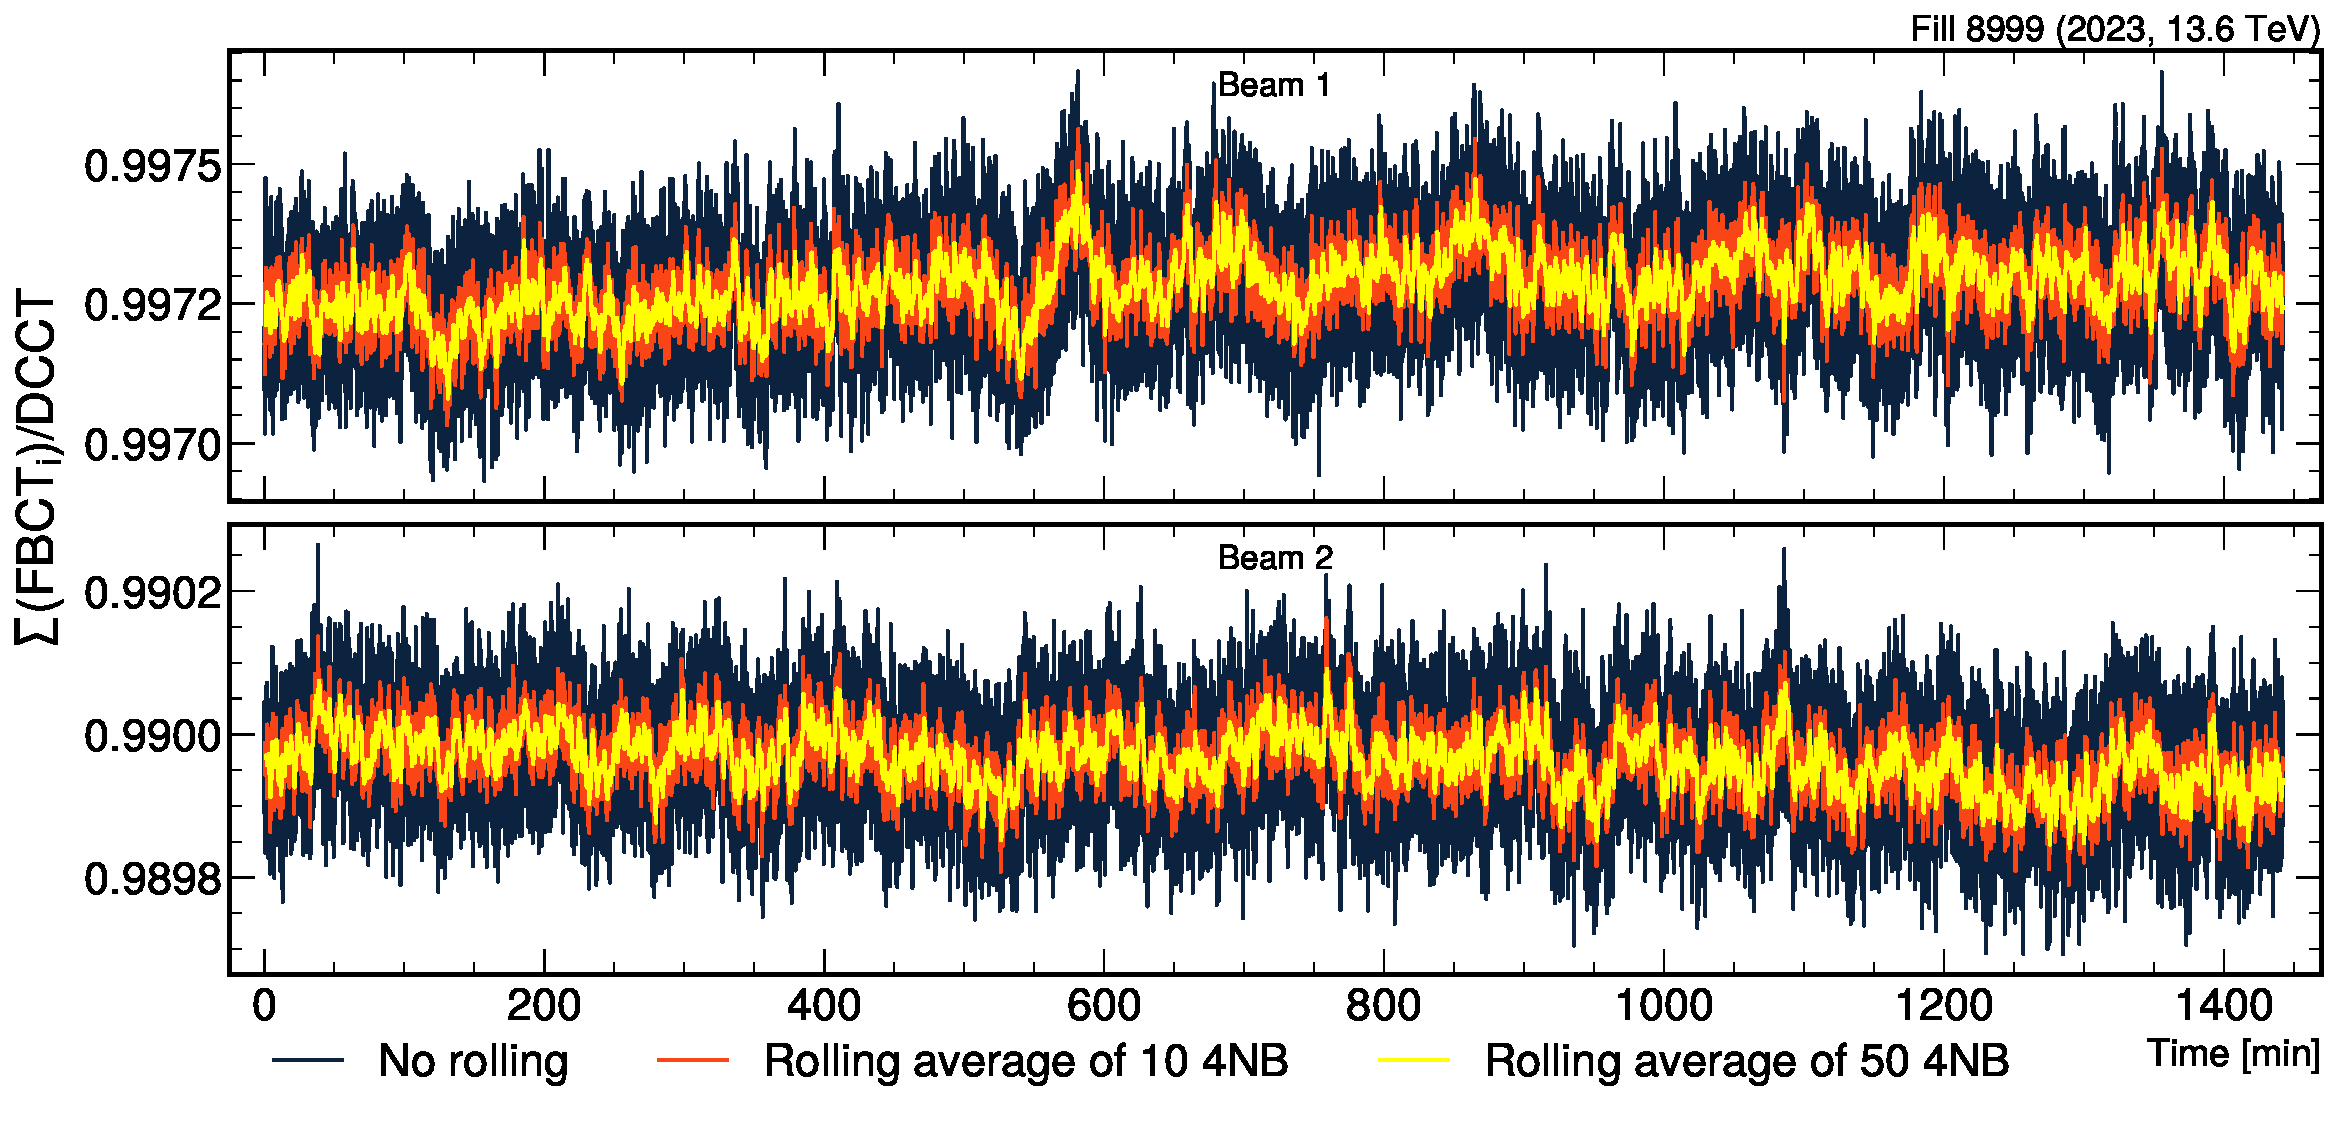
\includegraphics[width=0.8\paperwidth]{images/assets/fbct_dcct_calibration.pdf}}
	\caption[FBCT to DCCT calibration]{Value of the FBCT to DCCT calibration throughout the vdM fill 8999. The calibration factor is computed as the ratio between the orbit-integrated FBCT measurements and that of DCCT.}
	\label{fig:fbct_dcct_calibration}
\end{figure}

The FBCT system is able to provide current measurements with per-bunch granularity (every 25ns) while DCCT provides orbit integrated measurements with an associated uncertainty of 0.2\% \cite{Barschel:2649533}, achieving higher levels of accuracy compared to FBCT \cite{Gras:1379466}. This motivates a calibration procedure in which the orbit-integrated FBCT measurements are normalized to the measurements from DCCT. \autoref{fig:fbct_dcct_calibration} shows the value of this calibration across the entire vdM fill for both beams.

The application of this correction is done only in the measurements that correspond to time intervals where a scan is being performed. The overall magnitude of this calibration is calculated as the average among all the scan steps. \autoref{fig:fbct_dcct_vdM1_calibration} shows the calibration used for the first vdM scan pair, vdM1.

\begin{figure}[!htb]
	\centering
	\makebox[\textwidth]{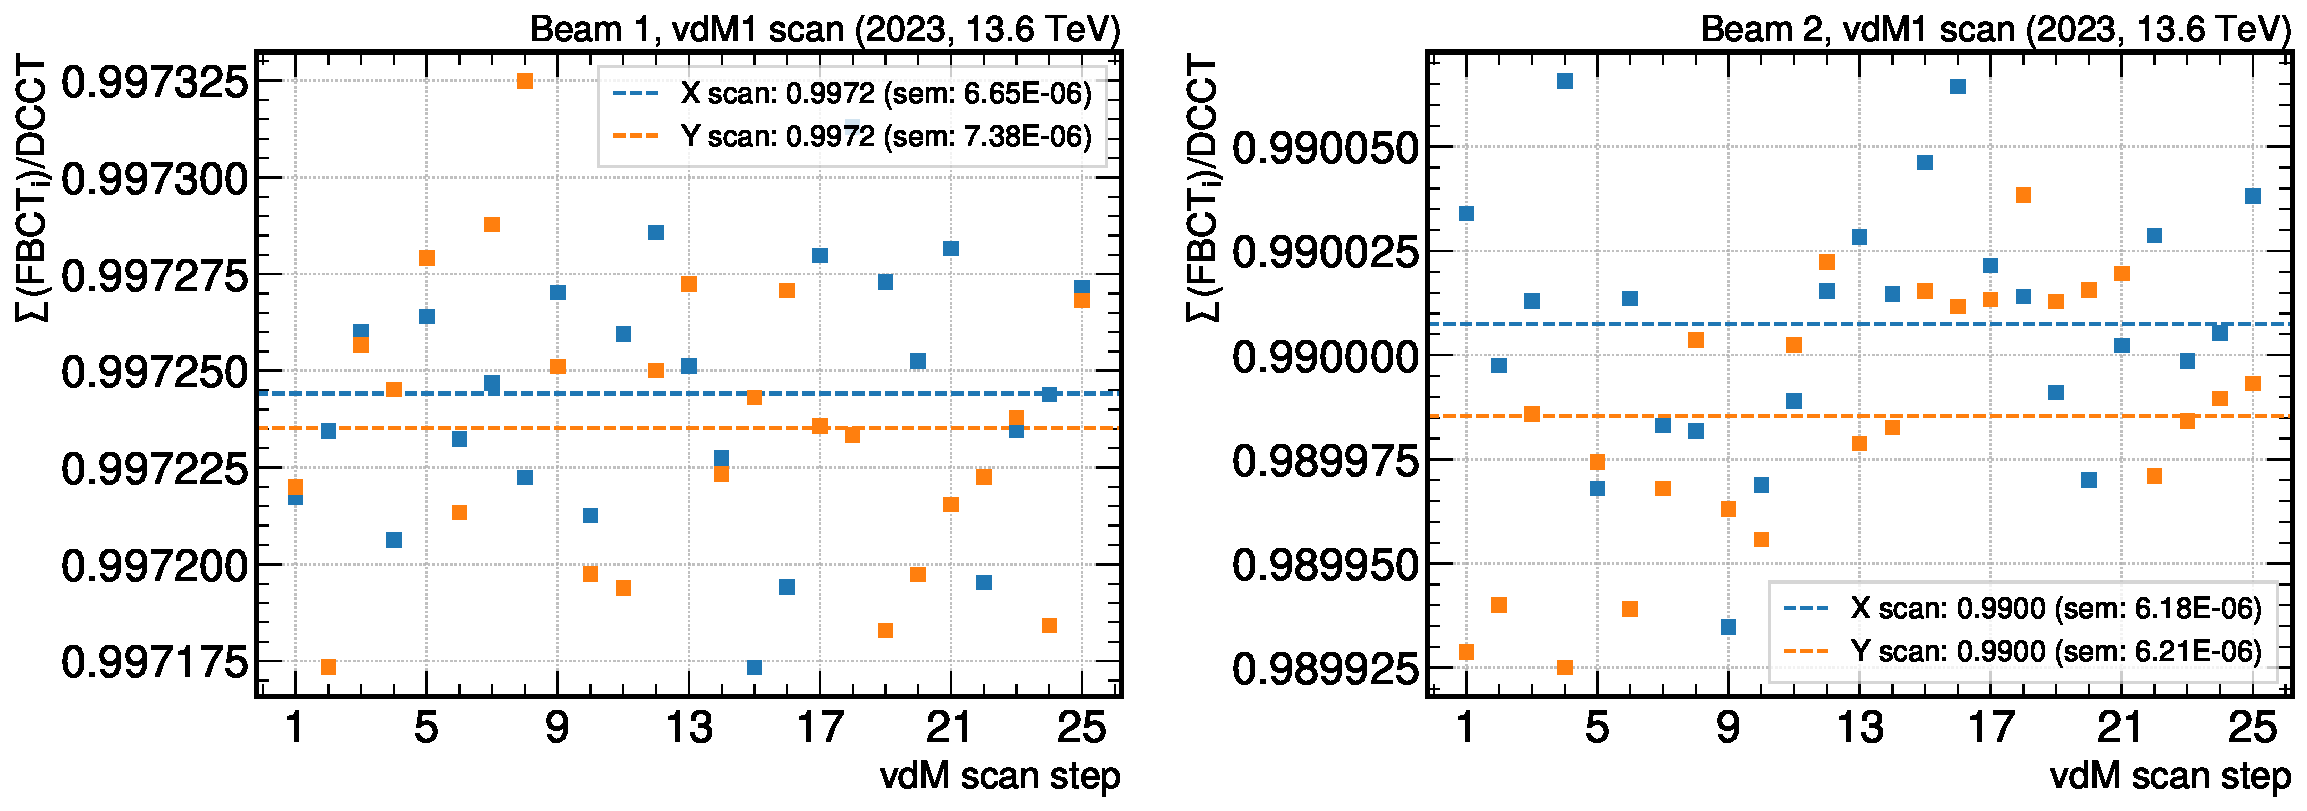
\includegraphics[width=0.8\paperwidth]{images/assets/fbct_dcct_vdM1_calibration.pdf}}
	\caption[FBCT calibration for scan pairs]{Calculated FBCT to DCCT calibration for the scan pairs of the first vdM scan in fill 8999. Every squared point corresponds to the ratio between the orbit-integrated FBCT beam current and the measurement from DCCT for a given scan step (25 in total for a vdM scan). The average and error on the mean are shown in the legend.}
	\label{fig:fbct_dcct_vdM1_calibration}
\end{figure}

Both systems are also susceptible to the presence of erratic charges. As mentioned in \autoref{subsec:particle_beams_lhc} only one out of the 10 RF buckets in a bunch crossing are nominally filled. Spurious charges in the nominally empty buckets, referred to as ``ghost charges", have an impact on the DCCT measurements but do not have an effect on the per-bunch FBCT measurement, since it is impervious to charges below a given threshold. Another class of additional charges, called ``satellites", emerge in the RF buckets adjacent to the nominally filled one. These extra charges affect the FBCT measurements. \autoref{fig:ghost_satellite_illustration} illustrates the position of these charges in relation to the main bunch. 

\begin{figure}[!htb]
	\centering
	\makebox[\textwidth]{\includegraphics[width=0.6\paperwidth]{images/assets/ghost_satellite_illustration.png}}
	\caption[Longitudinal bunch profile with LDM]{Longitudinal profile taken with the LDM, in logarithmic scale. The ghost charges are evenly spread while the satellites are adjacent to the main bunch (from \textit{Ref.} \cite{Alici:1427728}).}
	\label{fig:ghost_satellite_illustration}
\end{figure}

The LHC Longitudinal Density Monitor (LDM) system, measures the fraction of ghost charges in the DCCT measurement, $f_{ghost}$, as well as the per-bunch satellite fractions in the FBCT measurements, $f_{sat_i}$. Combining the calibration procedure specified above with the corrections from these LDM measurements, the total correction to the beam current can be expressed as:
\begin{equation}
	n_{i} = \frac{\mathrm{FBCT}_i \left( 1 - f_{sat_i} \right) \cdot \mathrm{DCCT} \left( 1 - f_{ghost} \right)}{\sum_i \mathrm{FBCT}_i}
\end{equation}
where $n_{i}$ is the corrected current for BCID $i$.

These corrections have a similar effect on all luminometers. The FBCT to DCCT calibration decreased the visible cross section by 1.27\% with an associated uncertainty equal to that of the DCCT measurement, 0.2\%. The correction from ghost-satellite charges had a +0.1\% effect on the detector calibration and the full correction was taken as an uncertainty.

\subsection{Length scale calibration}

During a vdM scan pair, the beams perform 25 steps in both planes. The movement of these beams is controlled with a pair of steering dipoles located on either side of the IP. However, the scale of each step may differ from the nominally intended step length. For example, an intended nominal step of, say, 1 $\mu m$ may correspond to $0.99$ $\mu m$. This can be generalized for any nominal position, $x_{\mathrm{nom}}$, and the associated actual measurement, $x_{\mathrm{real}}$, as:
\begin{equation}
	x_{\mathrm{meas}} = \alpha x_{\mathrm{nom}}
\end{equation}
where $\alpha$ is called the length scale factor. This parameter encodes the first-order linear response of the magnets to the nominal input positions.

This correction revolves around the comparison between the nominal and actual beam spot positions. The beam spot is the overall distribution of the vertices reconstructed from tracks registered in the tracking detector and its position refers to the average of this position. The CMS tracker \cite{Sirunyan:2759951}, provides the actual beam spot measurements, $\overline{x^{\mathrm{real}}_{\mathrm{BS}}}$, and the nominal measurement assumes that the individual beam profiles are Gaussian and factorizable. Therefore, the beam spot is computed as the weighted average from the two beams as \cite{CMS-PAS-LUM-22-001}:
\begin{equation}
	\overline{x^{\mathrm{nom}}_{\mathrm{BS}}} = \frac{\overline{x_1}\sigma_{x1}^{-2} + \overline{x_2}\sigma_{x2}^{-2}}{\sigma_{x1}^{-2} + \sigma_{x2}^{-2}},
\end{equation}
and similarly for the y direction. The $\overline{x^{\mathrm{nom}}_{\mathrm{BS}}}$ is the nominal beam spot position and $\overline{x_1}$ and $\overline{x_2}$ are the means of the beam profiles.

In practice, the length scale scans, as shown in \autoref{fig:vdm_fill_program}, are used. There are two versions of these scans: constant length scale (cls) scans and variable length scale (vls) scans. The cls scans are made up of 2 stages: forward stage, when the beams are moved from negative to positive positions, and the backward stage, where the beams are moved from positive to negative positions. In the cls scan, the relative beam separations are kept constant. In the vls scans, we have a cycle repeating a total of five times. This cycle comprises the moments in which beam 1 is above beam 2 (Up), the beams are head-on and, lastly, when beam 1 is below beam 2 (Dn). \autoref{fig:length_scale_scans} shows the beam positions during the cls1 and vls1 scan pairs.

\begin{figure}[!htb]
	\centering
	\makebox[\textwidth]{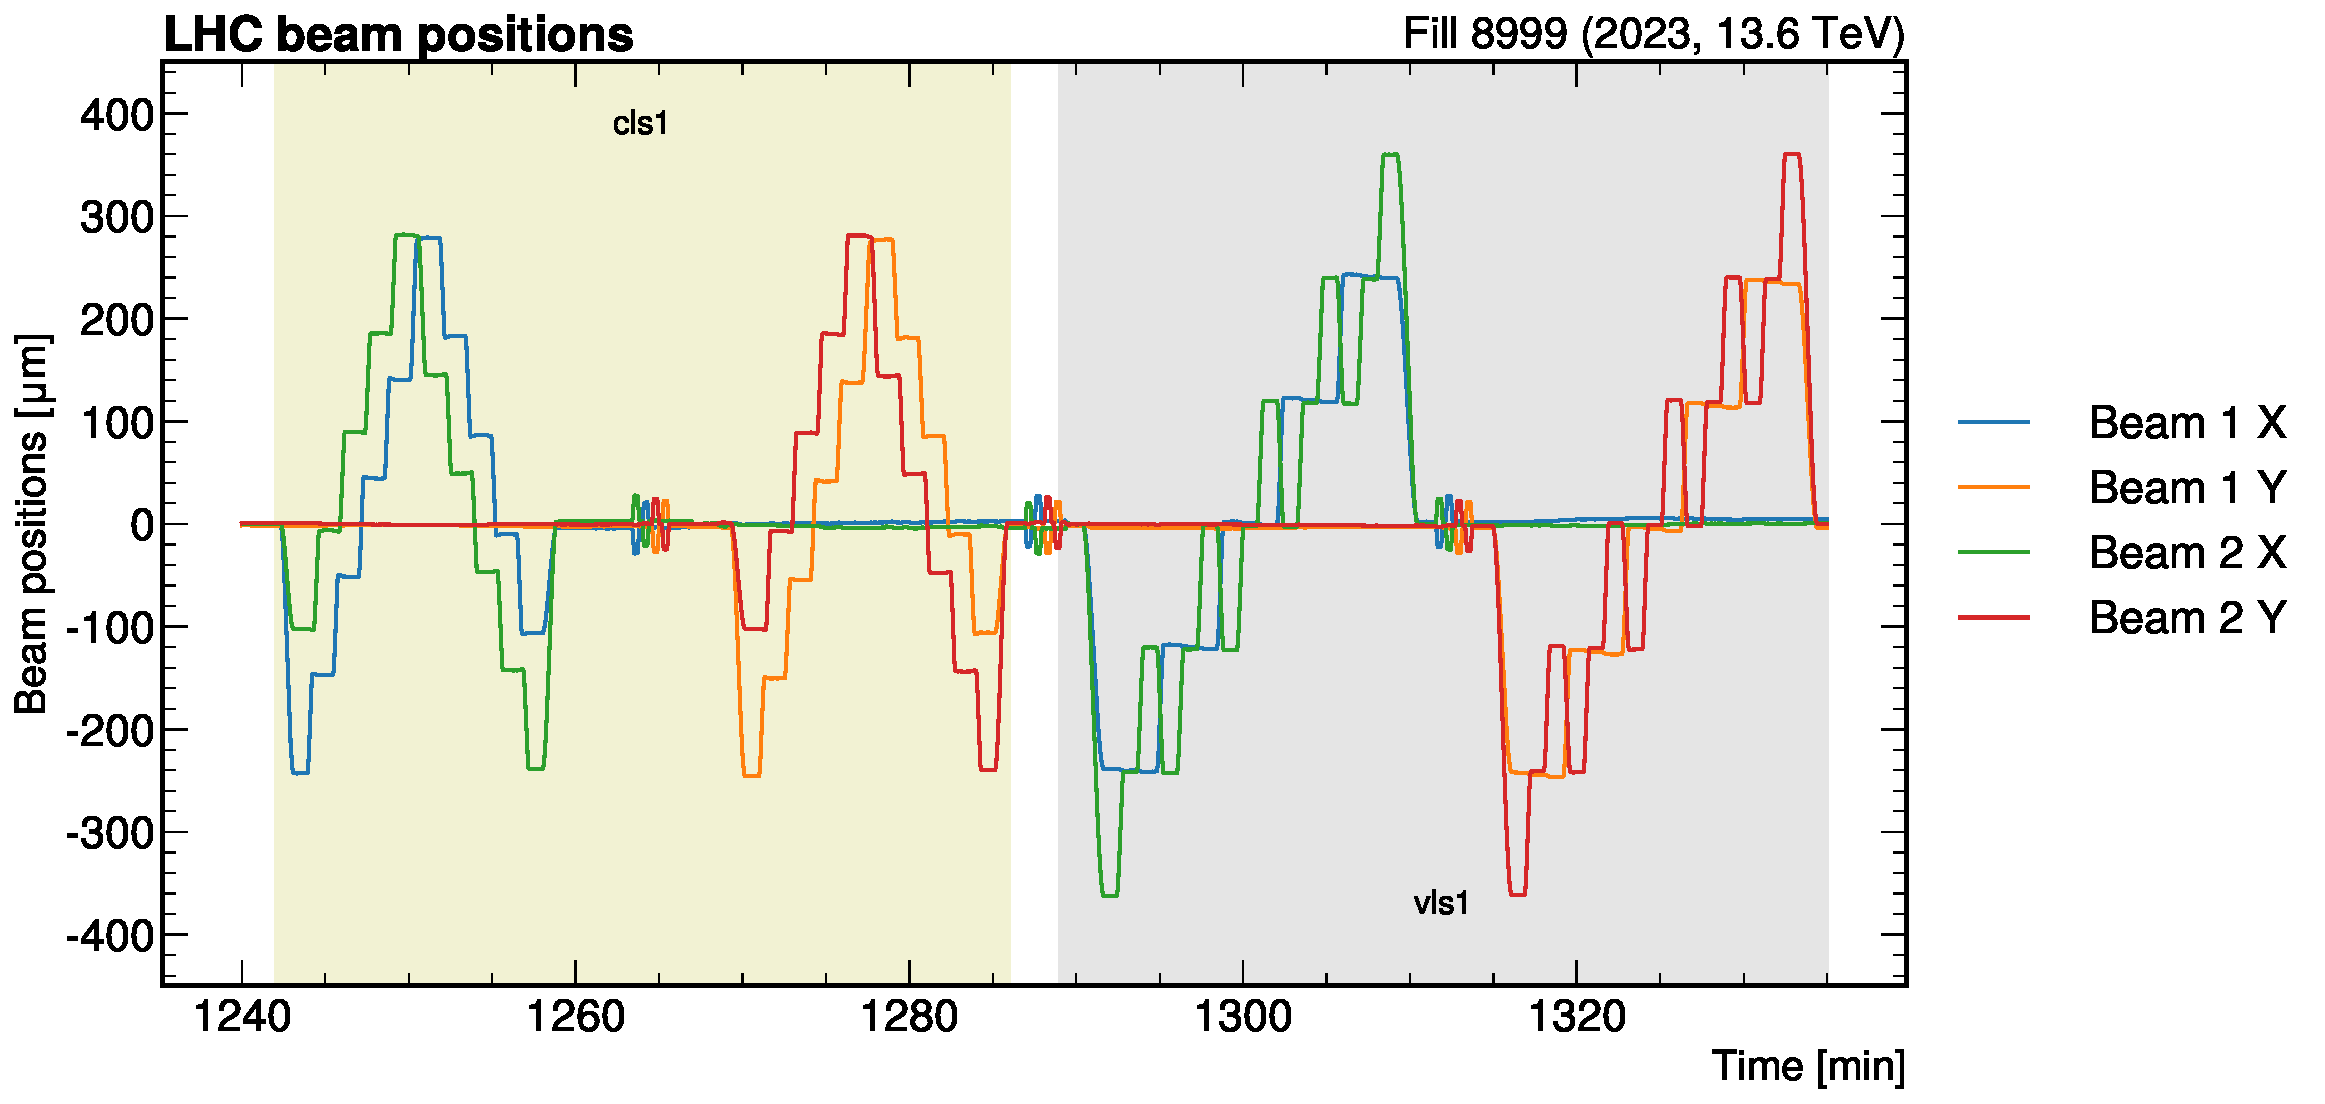
\includegraphics[width=0.6\paperwidth]{images/assets/length_scale_scans.pdf}}
	\caption[Beam positions in length scale scans]{Beam positions during the constant and variable length scale scans.}
	\label{fig:length_scale_scans}
\end{figure}

The difference between the real and nominal beam spot measurements are plotted as a function of the beam positions and a linear fit is performed to obtain the $\alpha$ factor. An example fit for the Up stage of the variable length scale scan is shown in \autoref{fig:fig:variable_length_scale_fit}. The overall length scale factor was calculated from a weighted average on the factors obtained from every possible scan and scan stage. The results are summarised in \autoref{fig:length_scale_fit_summary}.

\begin{figure}[!htb]
	\centering
	\makebox[\textwidth]{\includegraphics[width=0.4\paperwidth]{images/assets/variable_length_scale_fit.png}}
	\caption[Length scale factor determination]{Determination of the length scale factor $\alpha$ from a variable length scale scan (from \textit{Ref.} \cite{CMS-DP-2024-068}).}
	\label{fig:fig:variable_length_scale_fit}
\end{figure}

As the backward stage of the constant length scale for the vertical plane yielded poor quality fit results, it was not included in the weighted average. However, in order to account for this in the associated uncertainty, a systematic uncertainty was added to the already-obtained $0.0011$ RMS. This systematic was computed as the difference between the weighted average with and without this faulty scan stage and has an absolute value of $0.0012$. This results in a total uncertainty for the length scale factor in the y plane of $\sqrt{0.0011^2 + 0.0012^2} \approx 0.0016$.

The final uncertainty is the quadrature sum of the uncertainties in both planes, 0.2\%. The effect of this correction impacts all luminometers equally and resulted in a a decrease of the $\sigma_{\mathrm{vis}}$ of $0.9\%$.

\begin{figure}[h!]
	\centering
	\makebox[\textwidth]{\includegraphics[width=0.7\paperwidth]{images/assets/length_scale_fit_summary.png}}
	\caption[Length scale calibration results]{Results of the length scale calibration for the X (left) and Y (right) coordinates, using constant-separation length scale (cls) scans in the forward (fwd) and backward (bkw) directions, and variable-separation length scale (vls) scans (analysed as cls scans) for beam 1(2) scan with beam 2(1) (b2(b1)) being separated in the direction down (Dn) or up (Up) (from \textit{Ref.} \cite{CMS-DP-2024-068}). Length scale values are shown for fits whose reduced-$\chi^2$ is below 100, which was not the case for cls bkw scan in the Y plane.}
	\label{fig:length_scale_fit_summary}
\end{figure}

\subsection{Beam-beam effects}

When proton bunches collide at the IP, a repulsion force will be present due to their electromagnetic interaction. This interaction will have an effect on the luminometer rates, on the beam separations and, consequently, on the measured visible cross section. These effects, referred to as beam-beam effects, are corrected for in two ways.

As a consequence of the repulsive forces, the beam orbits will be deflected. The transverse electric field generated due to the interaction of the two particle bunches, $E(x, y)$, is calculated using the Bassetti-Erskine formula \cite{Bassetti:122227}. With the modelling of the transverse electric field, the deflection angle caused by electrostatic repulsion and the orbit shifts can be calculated with \autoref{eq:beam_deflection_angle} and \autoref{eq:beam_orbit_deflection} \cite{PhysRevLett.62.2949}, respectively.

\begin{equation}
	\theta_{\chi} = \frac{2r_p}{\gamma} N_p E_{\chi}(x, y), \, \mathrm{with} \, \chi \in \{ x, y \}
	\label{eq:beam_deflection_angle}
\end{equation}

\begin{equation}
	\delta_{\chi} = \frac{\theta_{\chi} \beta^{*}}{2 \mathrm{tan} \left( \pi Q_{\chi} \right)}, \, \mathrm{with} \, \chi \in \{ x, y \}
	\label{eq:beam_orbit_deflection}
\end{equation}

In these equations, $r_p$ is the classical proton radius, $N_p$ is the opposing bunch population, $\gamma$ is the relativistic factor and $Q_{\chi}$ is the betatron tune, a beam optics parameter specific to the each experiment. The calculated orbit deflections, $\delta_{\chi}$, are then used to correct the nominal beam separations for every bunch crossing and at each scan step.

When the bunches cross each other, the shape of the convoluted bunch distributions will also be affected by the electromagnetic interaction. This effect, commonly called dynamic-$\beta$ effect, is the second beam-beam effect that is taken into account. The distorted beam overlap shape will be reflected in a $\beta^{*}$ value different from the nominal one, which describes the envelope of the beam's transverse emittance and will affect the measured rates. This way, a corrective factor is multiplied to the measured rates in order to account for this effect. The magnitude of both corrections, beam-beam deflection and dynamic-$\beta$, are shown in \autoref{fig:beam_effects_correcions}.

\begin{figure}[!htb]
	\centering
	\makebox[\textwidth]{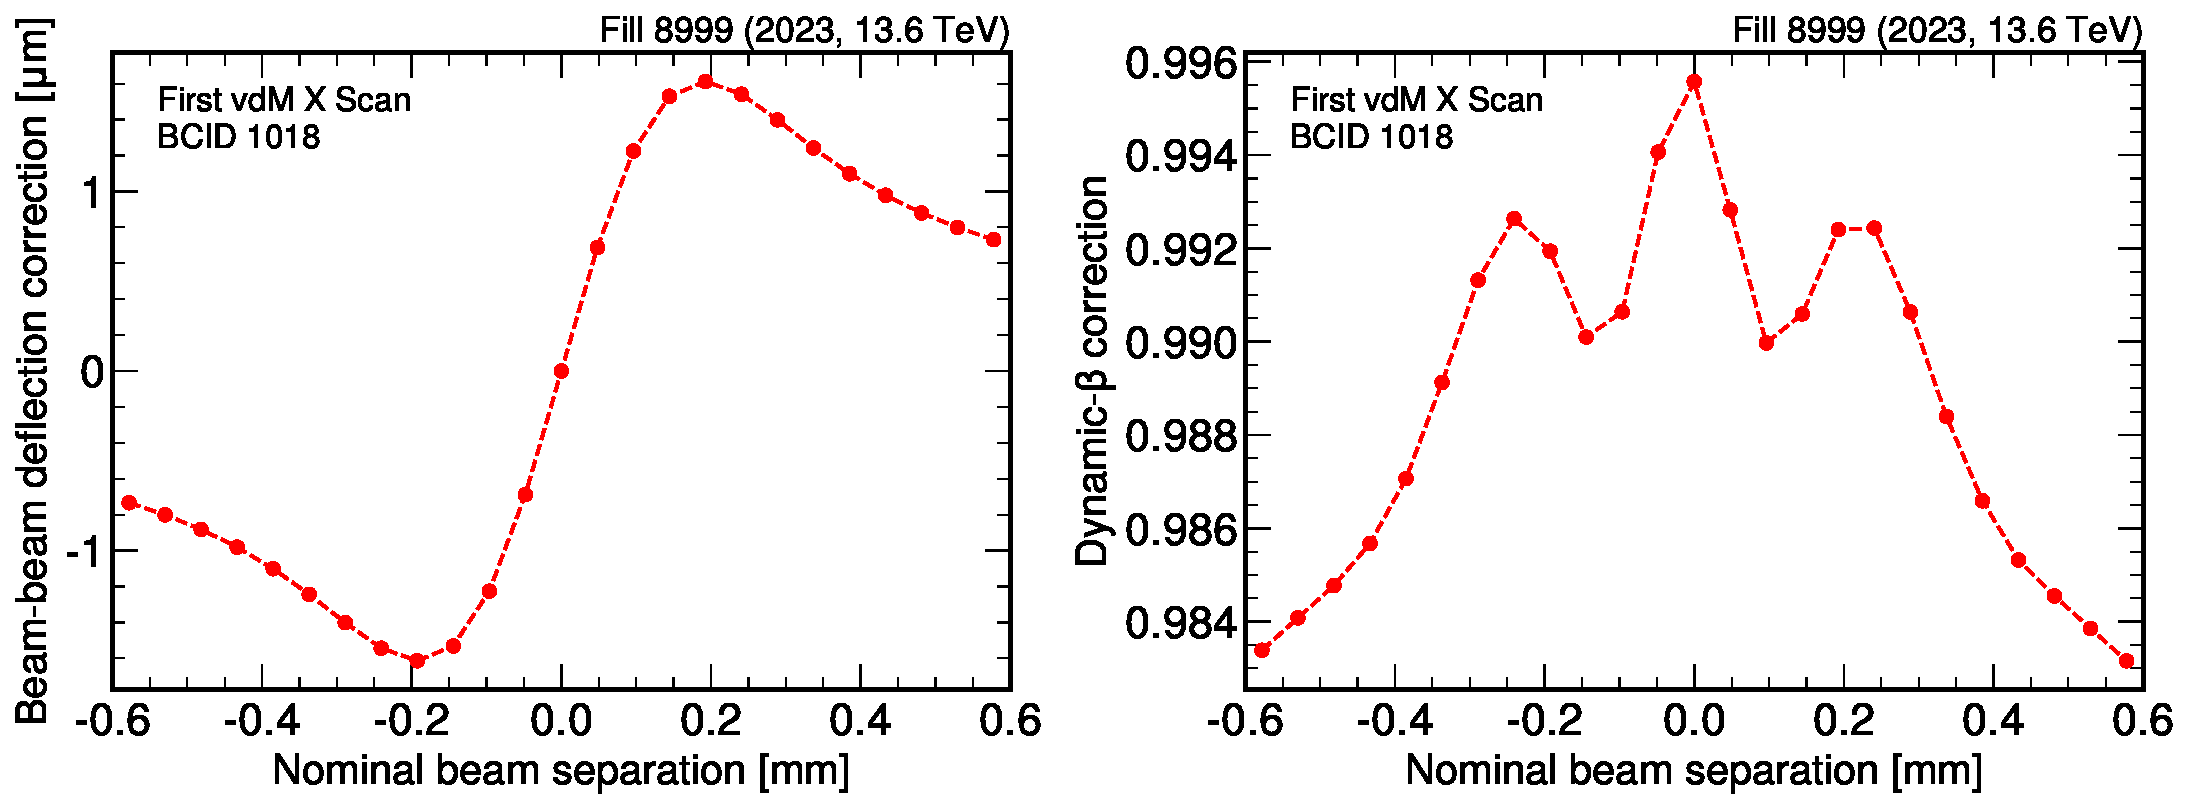
\includegraphics[width=0.7\paperwidth]{images/assets/beam_effects_correcions.pdf}}
	\caption[Electromagnetic interaction correction]{Correction values for the electromagnetic interaction between the 2 bunches. On the left, the orbit deflections due to electromagnetic repulsion are shown while on the right, the rate correction factors due to the distortion of the beam overlap shape are depicted.}
	\label{fig:beam_effects_correcions}
\end{figure}

Applying these corrections to all vdM and im scans yields an increase in $\sigma_{\mathrm{vis}}$ of 0.7\% for all luminometers. The associated uncertainty is computed from the quadrature sum of all the relevant sources of uncertainty summarised in \autoref{tb:beam_beam_uncertainty_summary}. A more detailed explanation of the beam-effects, the corrections and their associated uncertainties can be found in \cite{babaev2021coherentdeflectionellipticbunches}.

\begin{table}
	\centering
	\caption[Beam-beam systematic uncertainty]{Contributions to total beam-beam systematic uncertainty. Detailed description of these sources can be found in \cite{babaev2021coherentdeflectionellipticbunches}}\label{tab:bb:1}
	\label{tb:beam_beam_uncertainty_summary}
	\begin{tabular}{l|c}
		\hline
		Source & Uncertainty (\%) \\
		\hline
		Nominal tunes & 0.15 \\
		$\beta^{*}$ at IP5 & 0.11 \\
		Non-Gaussian tails & 0.16 \\
		Beam size imbalance & 0.01 \\
		Reference ambiguity & 0.20 \\
		Multi-IP tune shift & 0.04 \\
		Ellipticity & 0.03 \\
		Polynomial & 0.10 \\
		\hline
		Total & 0.34 \\
		\hline
	\end{tabular}
\end{table}

\subsection{Orbit drift}

Any drift in the beam positions, be it random or systematic, will result in a discrepancy from the nominal positions and, consequently, affect the visible cross section measurements. To correct for this effect, two beam position monitor systems (BPM) are used: the Diode Orbit and Oscillation System (DOROS) \cite{Gąsior:2313935} and the BPMs located in the LHC arcs (arcBPM) \cite{Sirunyan:2759951}.

The correction applied to the nominal beam positions, using the measurements from both BPMs, is done in two steps.

\begin{itemize}
	\item \textbf{Linear orbit drift}: In this correction, BPM measurements that are taken immediately before and after the scans, when the beam are in their nominal head-on positions, are used to determine the linear orbit drift at each step of a scan. To this effect, a linear interpolation is performed between these two points for every scan and the nominal positions are corrected accordingly. \autoref{fig:linear_orbit_drift_vdm1x} shows this procedure applied to the first vdM scan done in the horizontal transverse direction and \autoref{fig:linear_orbit_drift_correction} illustrates the orbit drift for all vdM and im scan pairs.

	\begin{figure}[!htb]
		\centering
		\makebox[\textwidth]{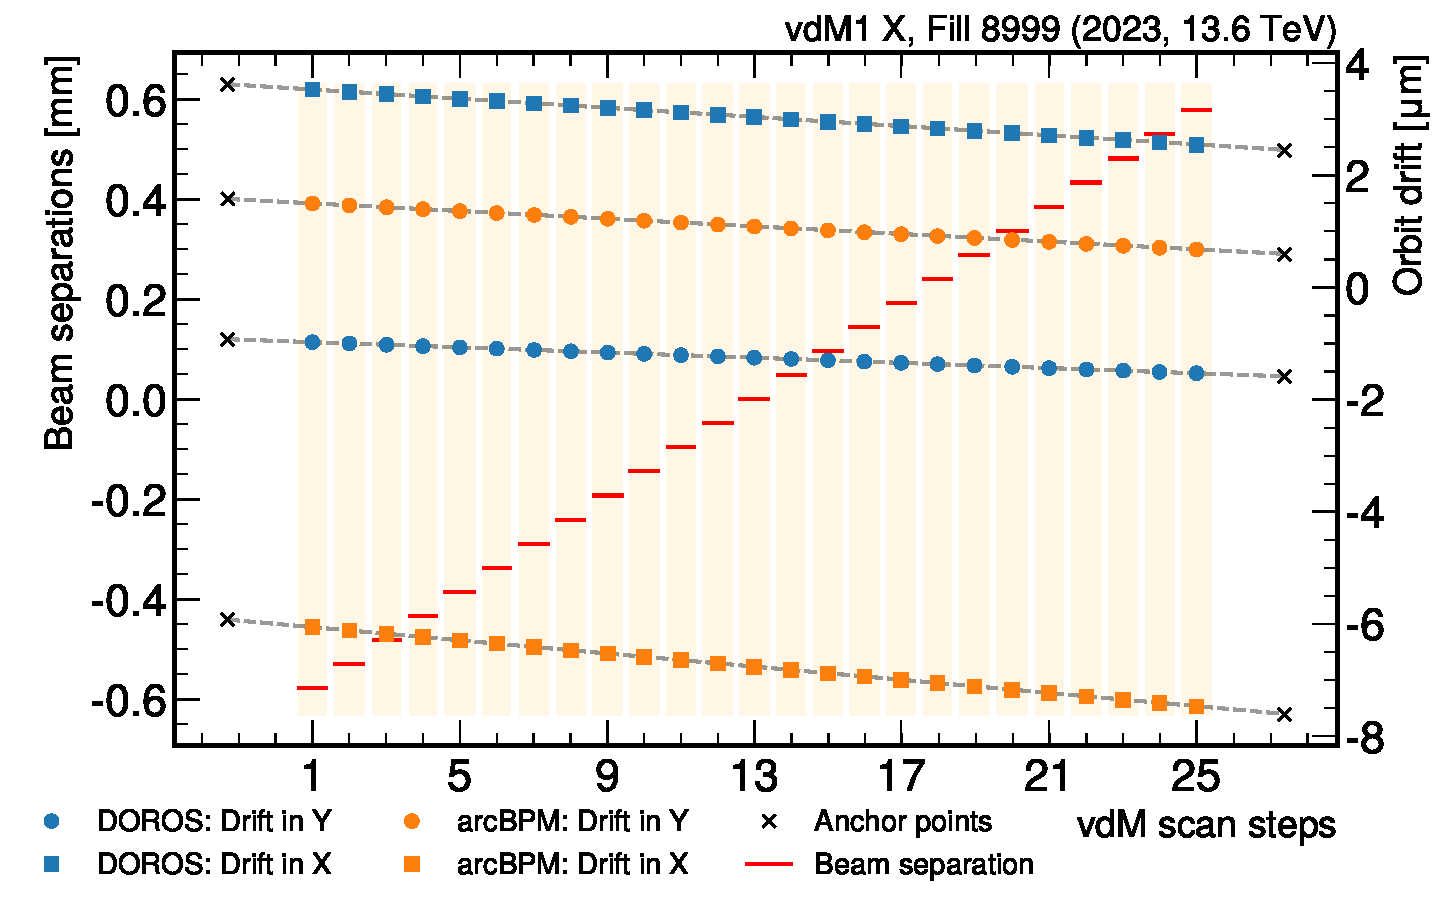
\includegraphics[width=0.6\paperwidth]{images/assets/linear_orbit_drift_vdm1x.pdf}}
		\caption[Orbit drift correction calculation]{Orbit drift correction calculated from the interpolation of the BPM measurements done before and after the vdM1 scan in the horizontal plane. The nominal beam separations (left axis), at every scan step and in $mm$,  are represented by the solid red lines, the interpolated points can be seen as black crosses. The linear interpolation was conducted for both BPM systems, DOROS (blue) and arcBPM (orange), and both planes, horizontal (squares) and vertical (circles). The orbit drifts (right axis) are expressed in $\mu m$.}
		\label{fig:linear_orbit_drift_vdm1x}
	\end{figure}

	\begin{figure}[!htb]
		\centering
		\makebox[\textwidth]{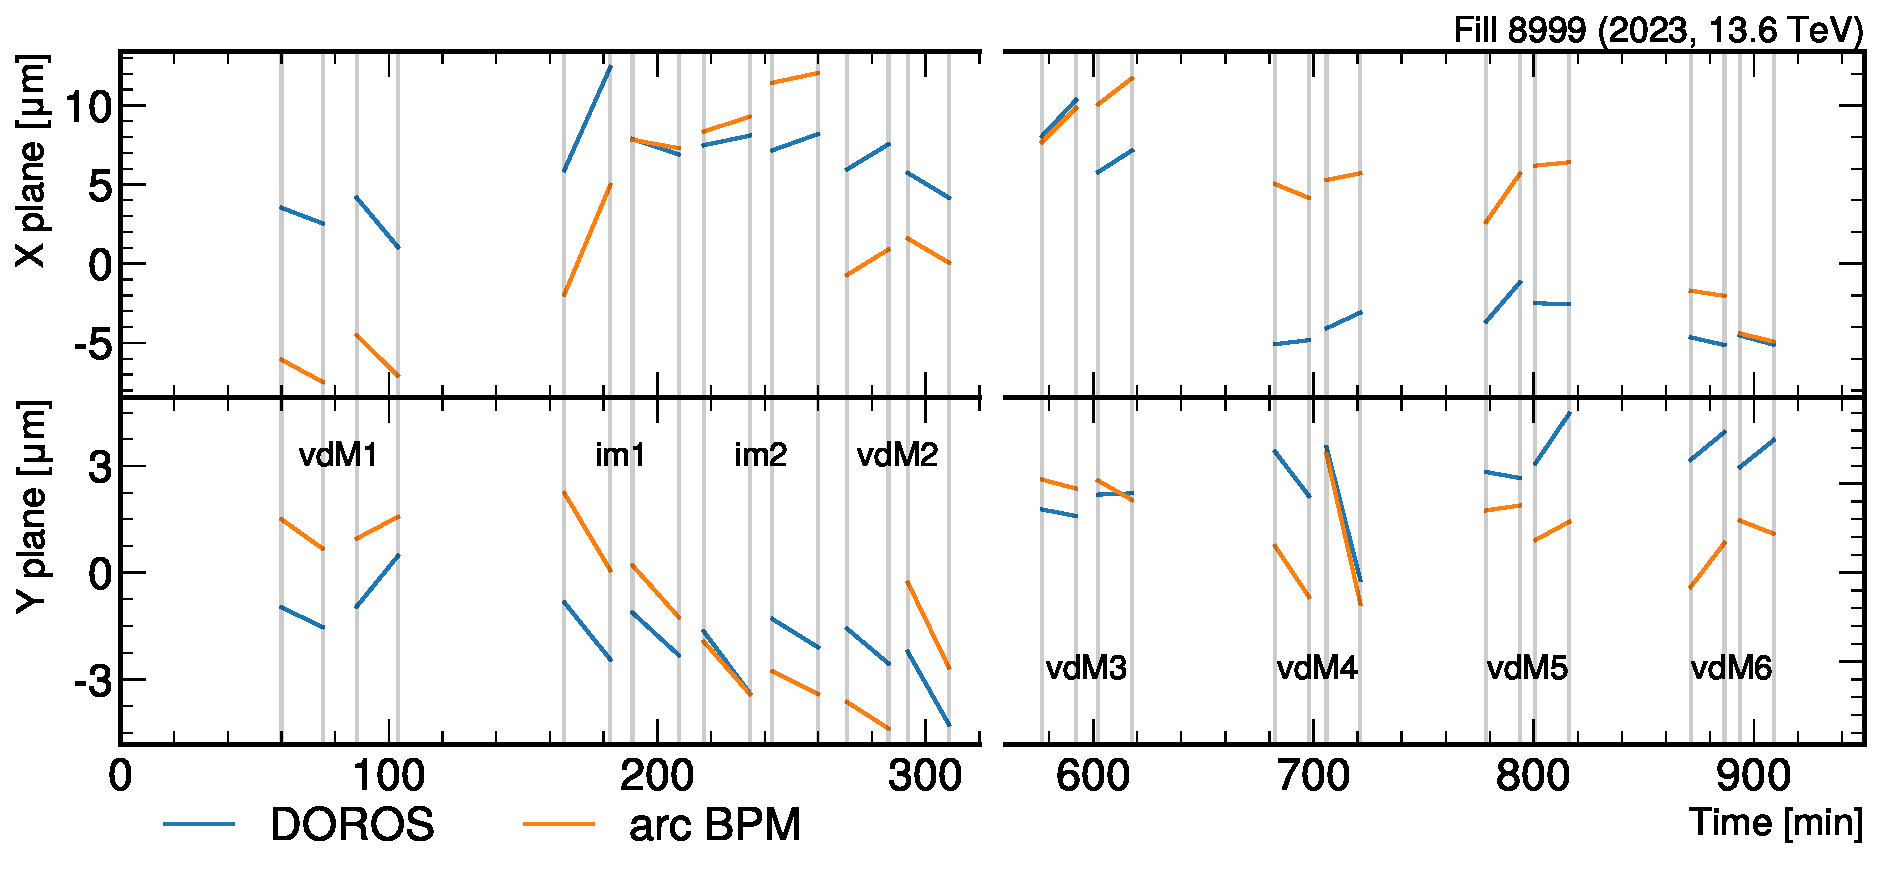
\includegraphics[width=0.8\paperwidth]{images/assets/linear_orbit_drift_correction.pdf}}
		\caption[Orbit drift correction summary]{Orbit drift correction for all vdM and im scan pairs.}
		\label{fig:linear_orbit_drift_correction}
	\end{figure}

	After correcting for the orbit drift in the nominal beam separations, we follow up with a correction to the measured rates in the non-scanning direction. To understand why, let us recall our assumption that the particle bunch distributions are XY-factorizable. Under this assumption, the rates measured in some arbitrary $(x, y)$ point would be:
	\begin{equation}
		R\left( x, y \right) = r_x(x) \cdot r_y(y).
	\end{equation}
	Taking the vertical plane as non-scanning, for example, an orbit drift ($\Delta_y$) would mean that our measured rates would be given as:
	\begin{equation}
		R\left( x, y + \Delta_y \right) = r_x(x) \cdot r_y(y + \Delta_y).
	\end{equation}
	We can then combine both equations to arrive at the rate correction:
	\begin{equation}
		R\left( x, y\right) = R\left( x, y + \Delta_y \right) \cdot \frac{r_y(y)}{r_y(y + \Delta_y)}.
	\end{equation}

	\item \textbf{Residual orbit drift}: After the linear orbit drift correction is applied, some residual differences remain between the nominal and the BPM measured beam positions. The length scale and the beam-beam deflection corrections are part of this residual difference and are accounted for as described in the previous sections. To correct for the remaining unpredictable deviations the residual differences are fitted as follows:
    \begin{gather}
    \mathrm{BPM}_{\mathrm{scanning}} - \mathrm{linOD}_{\mathrm{scanning}} = \alpha \mathrm{NOM}_{\mathrm{scanning}} + \beta \mathrm{BB}(\Delta\mathrm{NOM_{\mathrm{scanning}}}) + c_{\mathrm{scanning}} \\
    \mathrm{BPM}_{\mathrm{stationary}} - \mathrm{linOD}_{\mathrm{stationary}} = \gamma \mathrm{NOM}_{\mathrm{scanning}} + \frac{\gamma}{\alpha} \beta \mathrm{BB}(\Delta\mathrm{NOM}_{\mathrm{scanning}}) + c_{\mathrm{stationary}}
    \end{gather}
    $\alpha$ encodes the length scale factor difference between the nominal positions and the BPM measurements, $\gamma$, referred to as the leakage parameter, deals with the apparent misalignment between the measured and the nominal coordinate system, $\beta$ is a multiplicative factor to the beam-beam deflection at the IP and $c$ is simply a constant factor. After extracting the fit parameters, the residual orbit drifts are calculated as:
    \begin{gather}
    \Delta x_{\mathrm{scanning}} = \mathrm{BPM}_{\mathrm{scanning}} - \mathrm{linOD}_{\mathrm{scanning}} - \alpha \mathrm{NOM}_{\mathrm{scanning}} - \beta \mathrm{BB}(\Delta\mathrm{NOM_{\mathrm{scanning}}}) \\
    \Delta x_{\mathrm{stationary}} = \mathrm{BPM}_{\mathrm{stationary}} - \mathrm{linOD}_{\mathrm{stationary}} - \gamma \mathrm{NOM}_{\mathrm{scanning}} - \frac{\gamma}{\alpha} \beta \mathrm{BB}(\Delta\mathrm{NOM}_{\mathrm{scanning}})
    \end{gather}

    The fittings were performed simultaneously on both equations and with different relaxation levels for the $\alpha$ and $\beta$ parameters. The methods were:
	\begin{itemize}
		\item \textbf{Separate fit (Sep)}: Every parameter was fitted separately for every scan in the vdM program.
		\item \textbf{Average BB (AvgBB)}: The $\beta$ parameter used in the residual calculation is the average among all vdM scans.
		\item \textbf{Common BB (ComBB)}: The $\beta$ parameter is fitted globally across the scans.
		\item \textbf{Common LS (ComLS)}: The $\alpha$ parameter is fitted globally across the scans.
		\item \textbf{Common LSBB (ComLSBB)}: ComBB and ComLS methods combined.
	\end{itemize}
	In all methods, the leakage parameter $\gamma$ and the constant $c$ are fitted separately. The per-scan step residual correction calculated with the fit parameters obtained from the CommonLSBB fit method are shown in \autoref{fig:dps_residual_orbit_drifts}.

	\begin{figure}[!htb]
		\centering
		\makebox[\textwidth]{\includegraphics[width=0.8\paperwidth]{images/assets/dps_residual_orbit_drifts.png}}
		\caption[Residual beam position corrections]{Residual beam position corrections as a function of the scan step number for each vdM scan estimated using the arc BPM data and performing a global fit to all scans, which assumes a common BPM length scale and a common scale factor for the beam-beam deflection amplitude after correcting for the slow linear orbit drift. The red (blue) lines represent the residuals for the beam moving from the negative (positive) to the positive (negative) direction with respect to the reference CMS coordinate system. The band is the uncertainty that is estimated from the standard deviation of the position measurements (performed every second) within a scan step (from \textit{Ref.} \cite{CMS-DP-2024-068}).}
		\label{fig:dps_residual_orbit_drifts}
	\end{figure}
\end{itemize}

Upon correcting the beam separations and the non-scanning beam rates for the linear orbit drift, the visible cross section results increased by 0.22\% and 0.26\% for the arcBPM and DOROS measurement, respectively. The uncertainty of this correction was taken as half the difference of the two implementations, 0.02\%. For the residual orbit drift corrections, the impact of all fit methods were compared. \autoref{fig:rod_xsec_methods_results} displays the comparison for the HFET luminometer as an example. The numerical results are shown in \autoref{tb:hfet_rod_xsec}.

\begin{figure}[!htb]
	\centering
	\makebox[\textwidth]{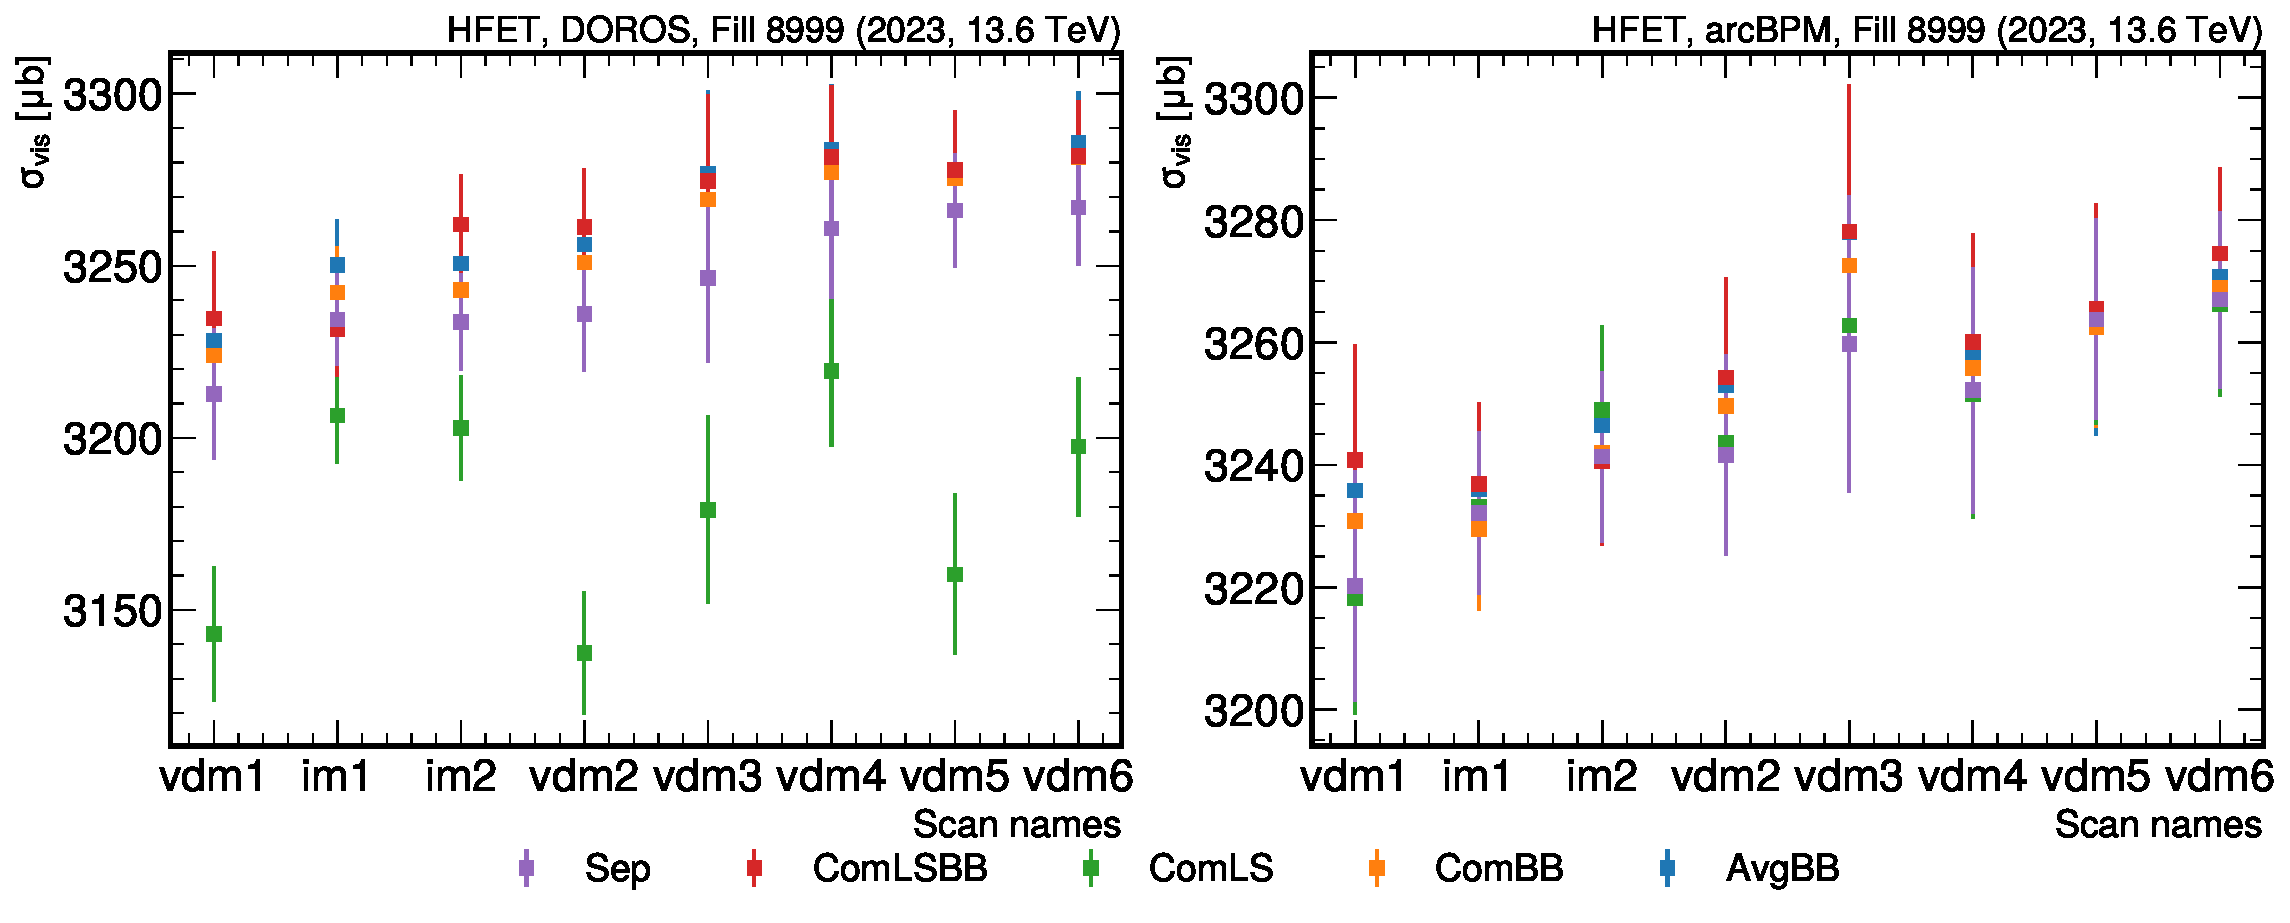
\includegraphics[width=0.8\paperwidth]{images/assets/rod_xsec_methods_results.pdf}}
	\caption[Comparison of residual orbit fit methods]{HFET visible cross section estimates for the vdM and im scan pairs after applying the orbit drift corrections. The central values are obtained by calculating the weighted average of the scan results. The scan to scan consistency is represented by the equivalent weighted standard deviation.}
	\label{fig:rod_xsec_methods_results}
\end{figure}

\begin{table}[!htb]
    \centering
    \caption{HFET visible cross sections for the many residual fit methods for both arcBPM and DOROS systems.}
    \label{tb:hfet_rod_xsec}
    \begin{tabular}{lcc|cc}
        \hline
        \multirow{2}{*}{Method} & \multicolumn{2}{c|}{DOROS} & \multicolumn{2}{c}{arcBPM} \\
        \cline{2-5}
         & $\sigma_{\mathrm{vis}}$ [$\mu b$] & Uncertainty (\%) & $\sigma_{\mathrm{vis}}$ [$\mu b$] & Uncertainty (\%) \\
        \hline
        Sep     & 3243.48 & 0.53 & 3246.49 & 0.47 \\
        AvgBB   & 3262.38 & 0.56 & 3252.75 & 0.42 \\
        ComLS   & 3183.52 & 0.91 & 3247.55 & 0.46 \\
        ComBB   & 3255.48 & 0.58 & 3249.46 & 0.47 \\
        ComLSBB & 3260.45 & 0.59 & 3254.09 & 0.46 \\
        \hline
    \end{tabular}
\end{table}


The results obtained from the separately-fit length scale parameter methods (Sep, AvgBB and ComBB) have not been considered since the length scale parameter as computed with the length scale calibration is constant throughout the vdM program. The ComLSBB method with the measurements from the arcBPM system was chosen for its smaller scan-to-scan variation (0.46\%). This correction increased the visible cross sections of all luminometers by 0.2\% with an associated uncertainty of 0.16\%, estimated from the standard deviation of results from all fits methods.

\subsection{XY factorization}

The assumption that the particle bunch distributions are factorizable in the transverse plane has been maintained throughout all the previously mentioned corrections. Since this assumption is not guaranteed, the visible cross section differs from the one measured with \autoref{eq:calibration_from_fit_parameters} by what is referred to as the factorization bias. This bias is calculated by reconstructing the bunch overlap densities of the two beams during the vdM fill and comparing the results to the ones obtained from the one-dimensional vdM scans.

Different methods are used for this purpose such as the beam-imaging method described in \cite{Klute_2017, knolle2019factorizationbiasvander, Knolle:442689}. For this analysis two other methods were used and their results were compared.

One of these methods is the 2D rate fit method, which has been carried out several times in previous CMS luminosity analyses \cite{CMS-PAS-LUM-18-002, CMS-PAS-LUM-22-001}. In this method, on-axis scans, like the previously mentioned vdM and im scans, are combined with off-axis scans, such as diagonal and offset scans, that were performed close in time. In diagonal scans, the scanning beam is moving in both the horizontal and vertical directions in such a way that the scanning plane is at a 45º angle. Offset scans are like normal vdM scans with an additional separation in the non-scanning plane. These off-axis scans are illustrated in \autoref{fig:off_axis_scans}.

\begin{figure}[!htb]
	\centering
	\makebox[\textwidth]{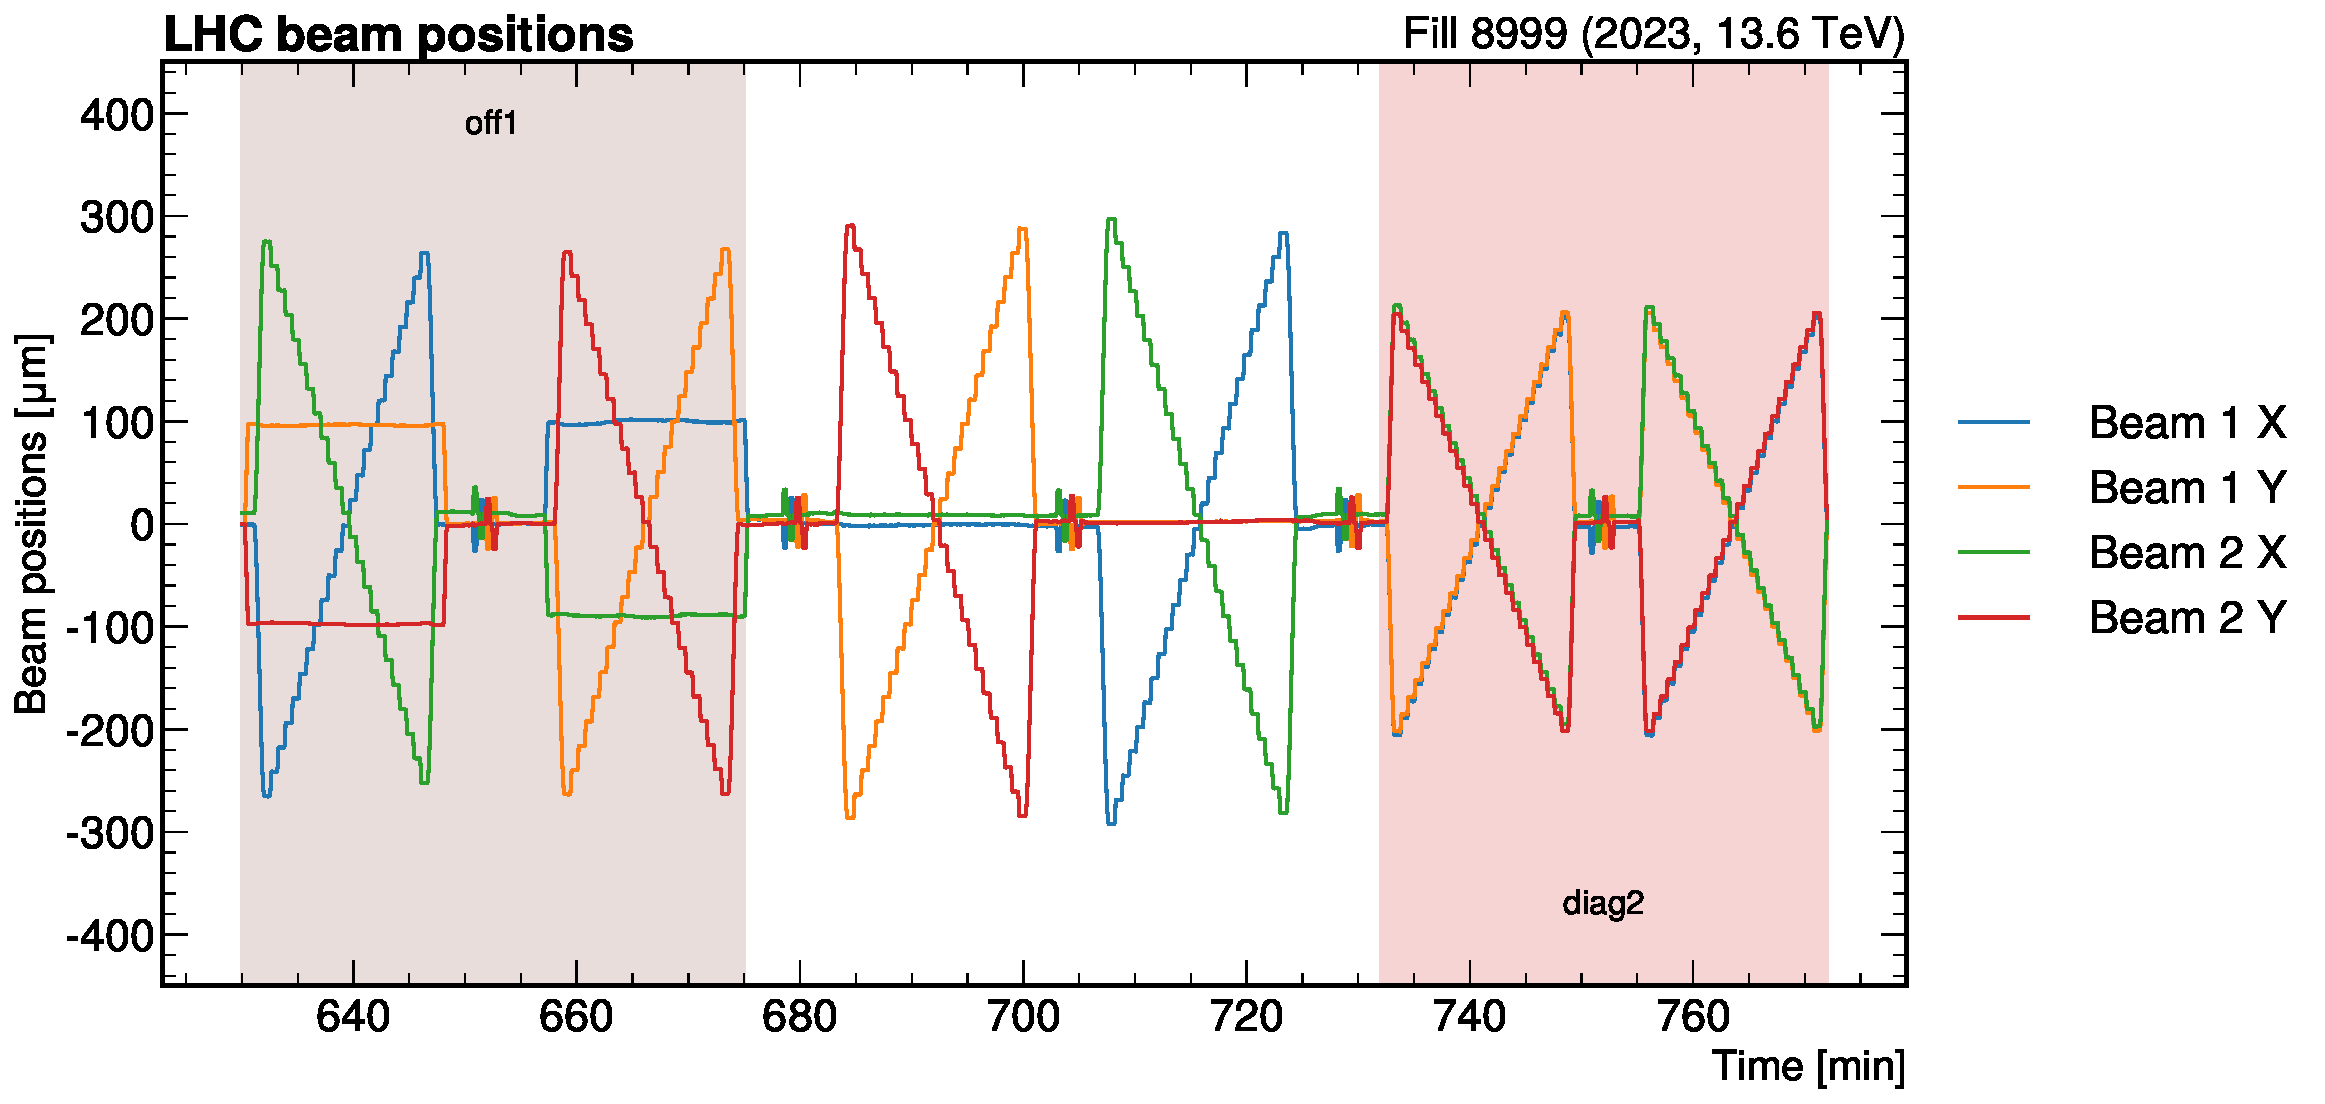
\includegraphics[width=0.8\paperwidth]{images/assets/off_axis_scans.pdf}}
	\caption{Beam positions during the first offset scan and the second diagonal scan of fill 8999.}
	\label{fig:off_axis_scans}
\end{figure}

The combination of on-axis with off-axis scans allows for the probing of the overlap bunch distribution along a different paths. This provides more information about the non-factorizable nature of this distribution. For 2023 vdM program, the scan combinations were vdM1+diag1, diag1+BI1, vdM3+off1, off1+vdM4, vdM4+diag2 and diag2+vdM5. The visible cross section corrections for all these combinations are shown in \autoref{fig:2d_rate_fit_xsec_corrections}.

\begin{figure}[!htb]
	\centering
	\makebox[\textwidth]{\includegraphics[width=0.4\paperwidth]{images/assets/2d_rate_fit_xsec_corrections.png}}
	\caption[Factorization corrections on visible cross section from 2D rate fit method]{Factorization corrections on the visible cross section from several on-axis scan and off-axis scan pairs as a function of time. The points from left to right correspond to vdM1+diag1, diag1+BI1 combinations taken during the first part of the vdM program (in brown), and to vdM3+off, off+vdM4, vdM4+diag2, diag2+vdM5 combinations taken during the second part of the vdM program (in purple). Over the nine hours of the data taking, the factorization correction changed from about 2.62\% to approximately 0.93\%, indicating a significant time dependence (from \textit{Ref.} \cite{CMS-DP-2024-068}).}
	\label{fig:2d_rate_fit_xsec_corrections}
\end{figure}

Lastly, a 3D fit in the luminous region is performed to luminometer rates using parameters of the 3D ellipsoid of the reconstructed beamspot and the bunch length data from the LHC LDM. One of the main advantages of this method, in comparison to the 2D rate method, is the ability to obtain a cross section measurement for every vdM and im scan separately. For this reason, the corrections to the detectors calibration were derived from this method. A comparison to the 2D rate fit method is shown in \autoref{fig:luminous_region_vs_2d_rate_fit}, which shows good agreement between both methods. The large time dependence in the correction values demonstrate the change in beam overlap shape throughout the vdM fill.

\begin{figure}[!htb]
	\centering
	\makebox[\textwidth]{\includegraphics[width=0.5\paperwidth]{images/assets/luminous_region_vs_2d_rate_fit.png}}
	\caption[Factorization corrections on visible cross section from luminous region method.]{Average correction for the visible cross section over nine BCIDs using five different models of the luminous region (LR) method. The scans are ordered in time. The averages include only BCIDs for which high-statistics zero bias samples are available, and the uncertainties indicate the RMS over these BCIDs. A small number of bad quality fits with anomalously large reduced $\chi^2$ > 5 were discarded. Results for three models of the bunch proton density are shown: weighted sum of three (TG), four (QG) or five (PG) 3-dimensional Gaussians. The results – choosing the best and the second best (i.e. smallest) reduced $\chi^2$ fits from the nine tested models – are also given. On the right, the LR results are compared to the average corrections over 136 BCIDs using the 2D rate fit method (from \textit{Ref.} \cite{CMS-DP-2024-068}).}
	\label{fig:luminous_region_vs_2d_rate_fit}
\end{figure}

The XY-factorization bias was the main responsible for reducing the scan-to-scan variation seen in \autoref{fig:no_Corr_xsec_results_HFET} and \autoref{fig:noCorr_luminometer_xsec}. The total uncertainty for this correction is 0.67\%, which was estimated from the uncertainty associated with model- and BCID-dependence and the maximum discrepancy with the 2D rate fit method, among other sources \cite{CMS-PAS-LUM-22-001}.

\subsection{Calibration results}

The visible cross section results were determined by performing a weighted average on the calibrations measured in the eight analyzed scans, incorporating all prior corrections. \autoref{tab:xsec_summary} provides a summary of the results for all independently calibrated luminometers, along with their associated uncertainties. The associated $\sigma_{\mathrm{vis}}$ evolution plots are in \autoref{fig:all_Corr_xsec_results_HFET} for the HFET detector and in \autoref{fig:all_Corr_luminometer_xsec} and \autoref{fig:cross_section_results_pcc} for the remaining luminometers.

\begin{table}[!htb]
	\caption[Summary of visible cross sections results]{Summary of the measured visible cross sections. The results have been computed through an average weighted on the error of each scan and are accompanied by their standard error on the mean. The bunch-to-bunch uncertainty range across all scans is shown in the "Bunches RMS" column. The "Scans RMS" depicts the overall scan-to-scan variation. }
	
	\label{tab:xsec_summary}
	\centering
	\begin{tabular}{lcccc}
		\hline
		Luminometer & Measured $\sigma_\mathrm{vis}$ & SEM  & Bunches RMS & Scans RMS \\
		\hline
		BCM1F & 136.36 $\mu b$ & 0.17 $\mu b$ & 0.58-1.03 $\mu b$ (0.43-0.76\%) & 0.41 $\mu b$ (0.30\%) \\
		BCM1FUTCA & 127.55 $\mu b$ & 0.15 $\mu b$ & 0.61-1.09 $\mu b$ (0.48-0.85\%) & 0.40 $\mu b$ (0.31\%) \\
		HFET & 3294.69 $\mu b$ & 3.86 $\mu b$ & 12.82-21.78 $\mu b$ (0.39-0.66\%) & 9.28 $\mu b$ (0.28\%) \\
		HFOC & 946.05 $\mu b$ & 1.12 $\mu b$ & 2.49-5.92 $\mu b$ (0.26-0.63\%) & 2.63 $\mu b$ (0.28\%) \\
		PLT & 301.39 $\mu b$ & 0.37 $\mu b$ & 1.52-2.38 $\mu b$ (0.50-0.79\%) & 0.90 $\mu b$ (0.30\%) \\
		PCC & 1305.23 $mb$ & 1.21 $mb$ & 3.31-8.85 $mb$ (0.25-0.68\%) & 3.27 $mb$ (0.25\%) \\
		\hline
	\end{tabular}
\end{table}

\begin{figure}[!htb]
	\centering
	\makebox[\textwidth]{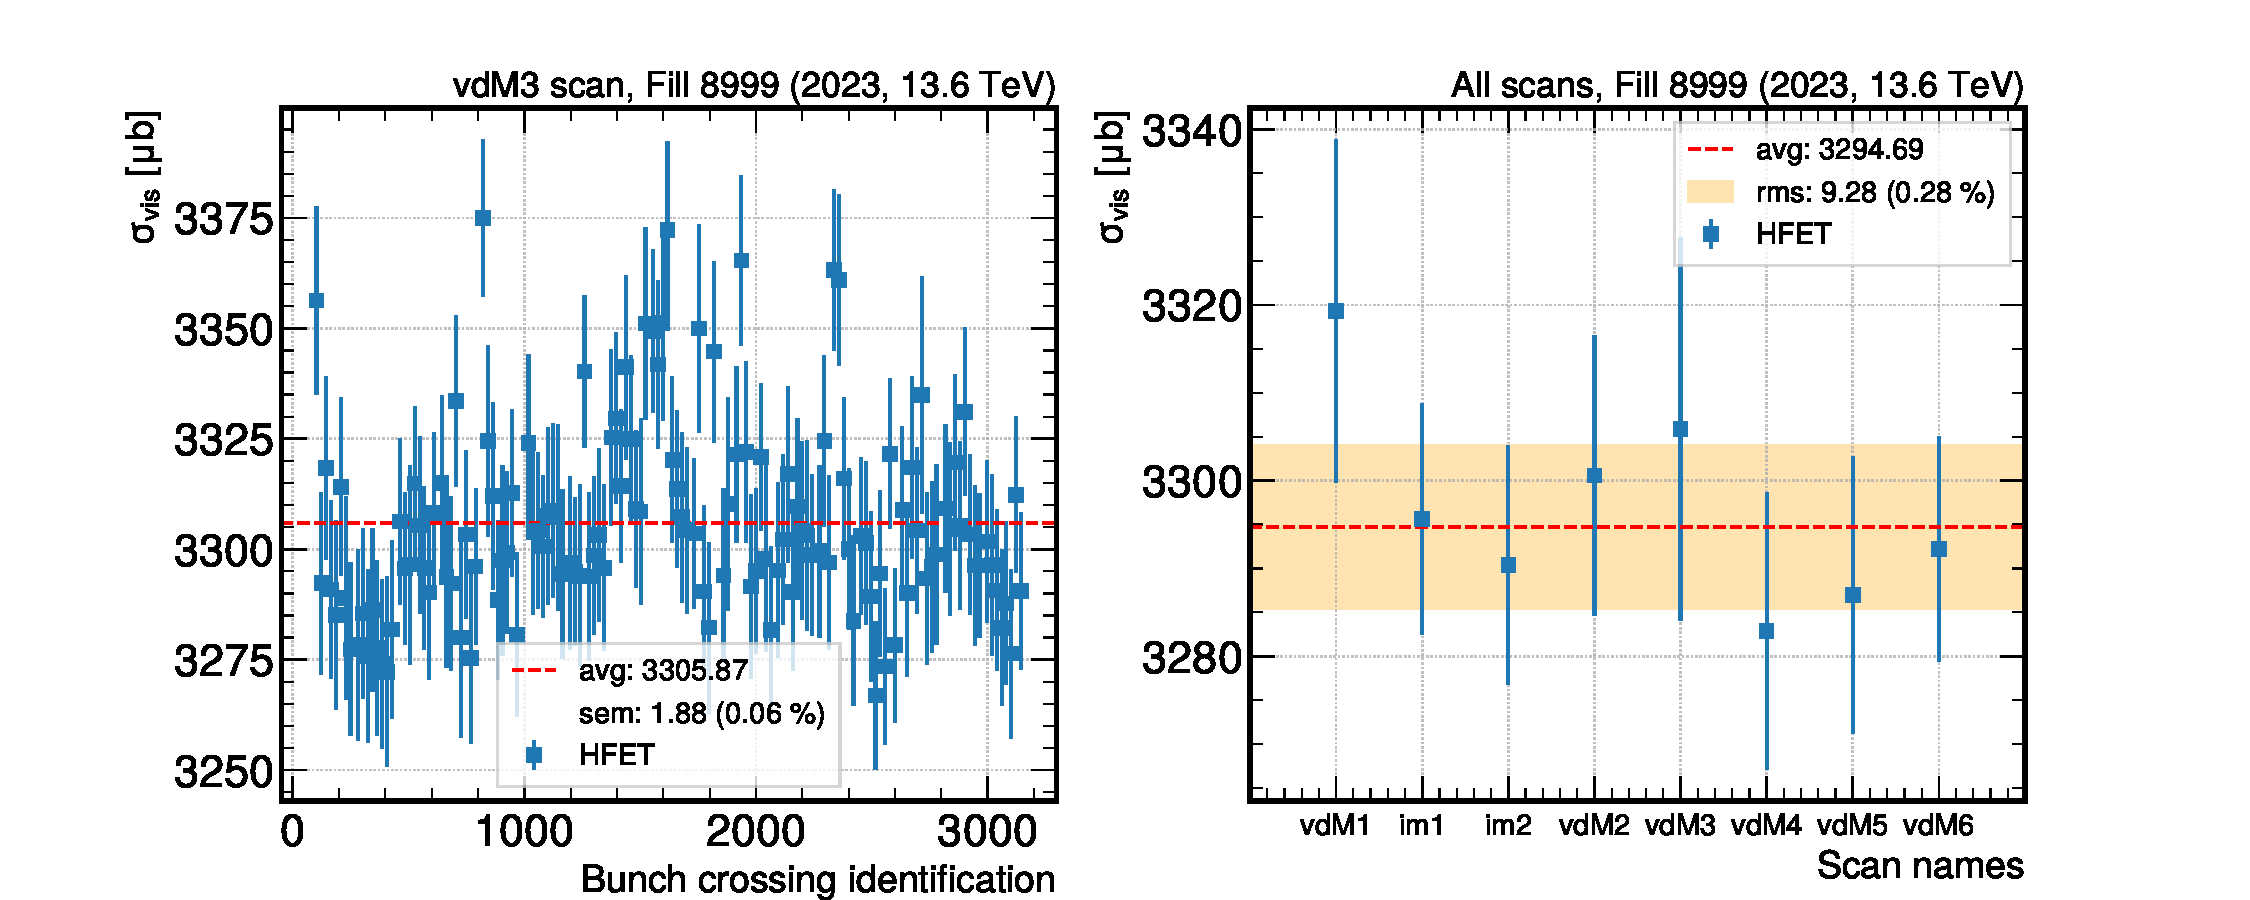
\includegraphics[width=0.9\paperwidth]{images/assets/all_Corr_xsec_results_HFET.pdf}}
	\caption[Final HFET visible cross section results]{Final visible cross section results obtained after all data corrections for the HFET luminometer, as an example. On the left, the measured per-bunch visible cross sections with its associated fit uncertainty are shown. The right image shows the measured visible cross section taking the average over all 136 colliding BCIDs for each vdM and im scan pairs. All statistics are determined as in \autoref{fig:no_Corr_xsec_results_HFET}.}
	\label{fig:all_Corr_xsec_results_HFET}
\end{figure}

\begin{figure}[!htb]
	\centering
	\makebox[\textwidth]{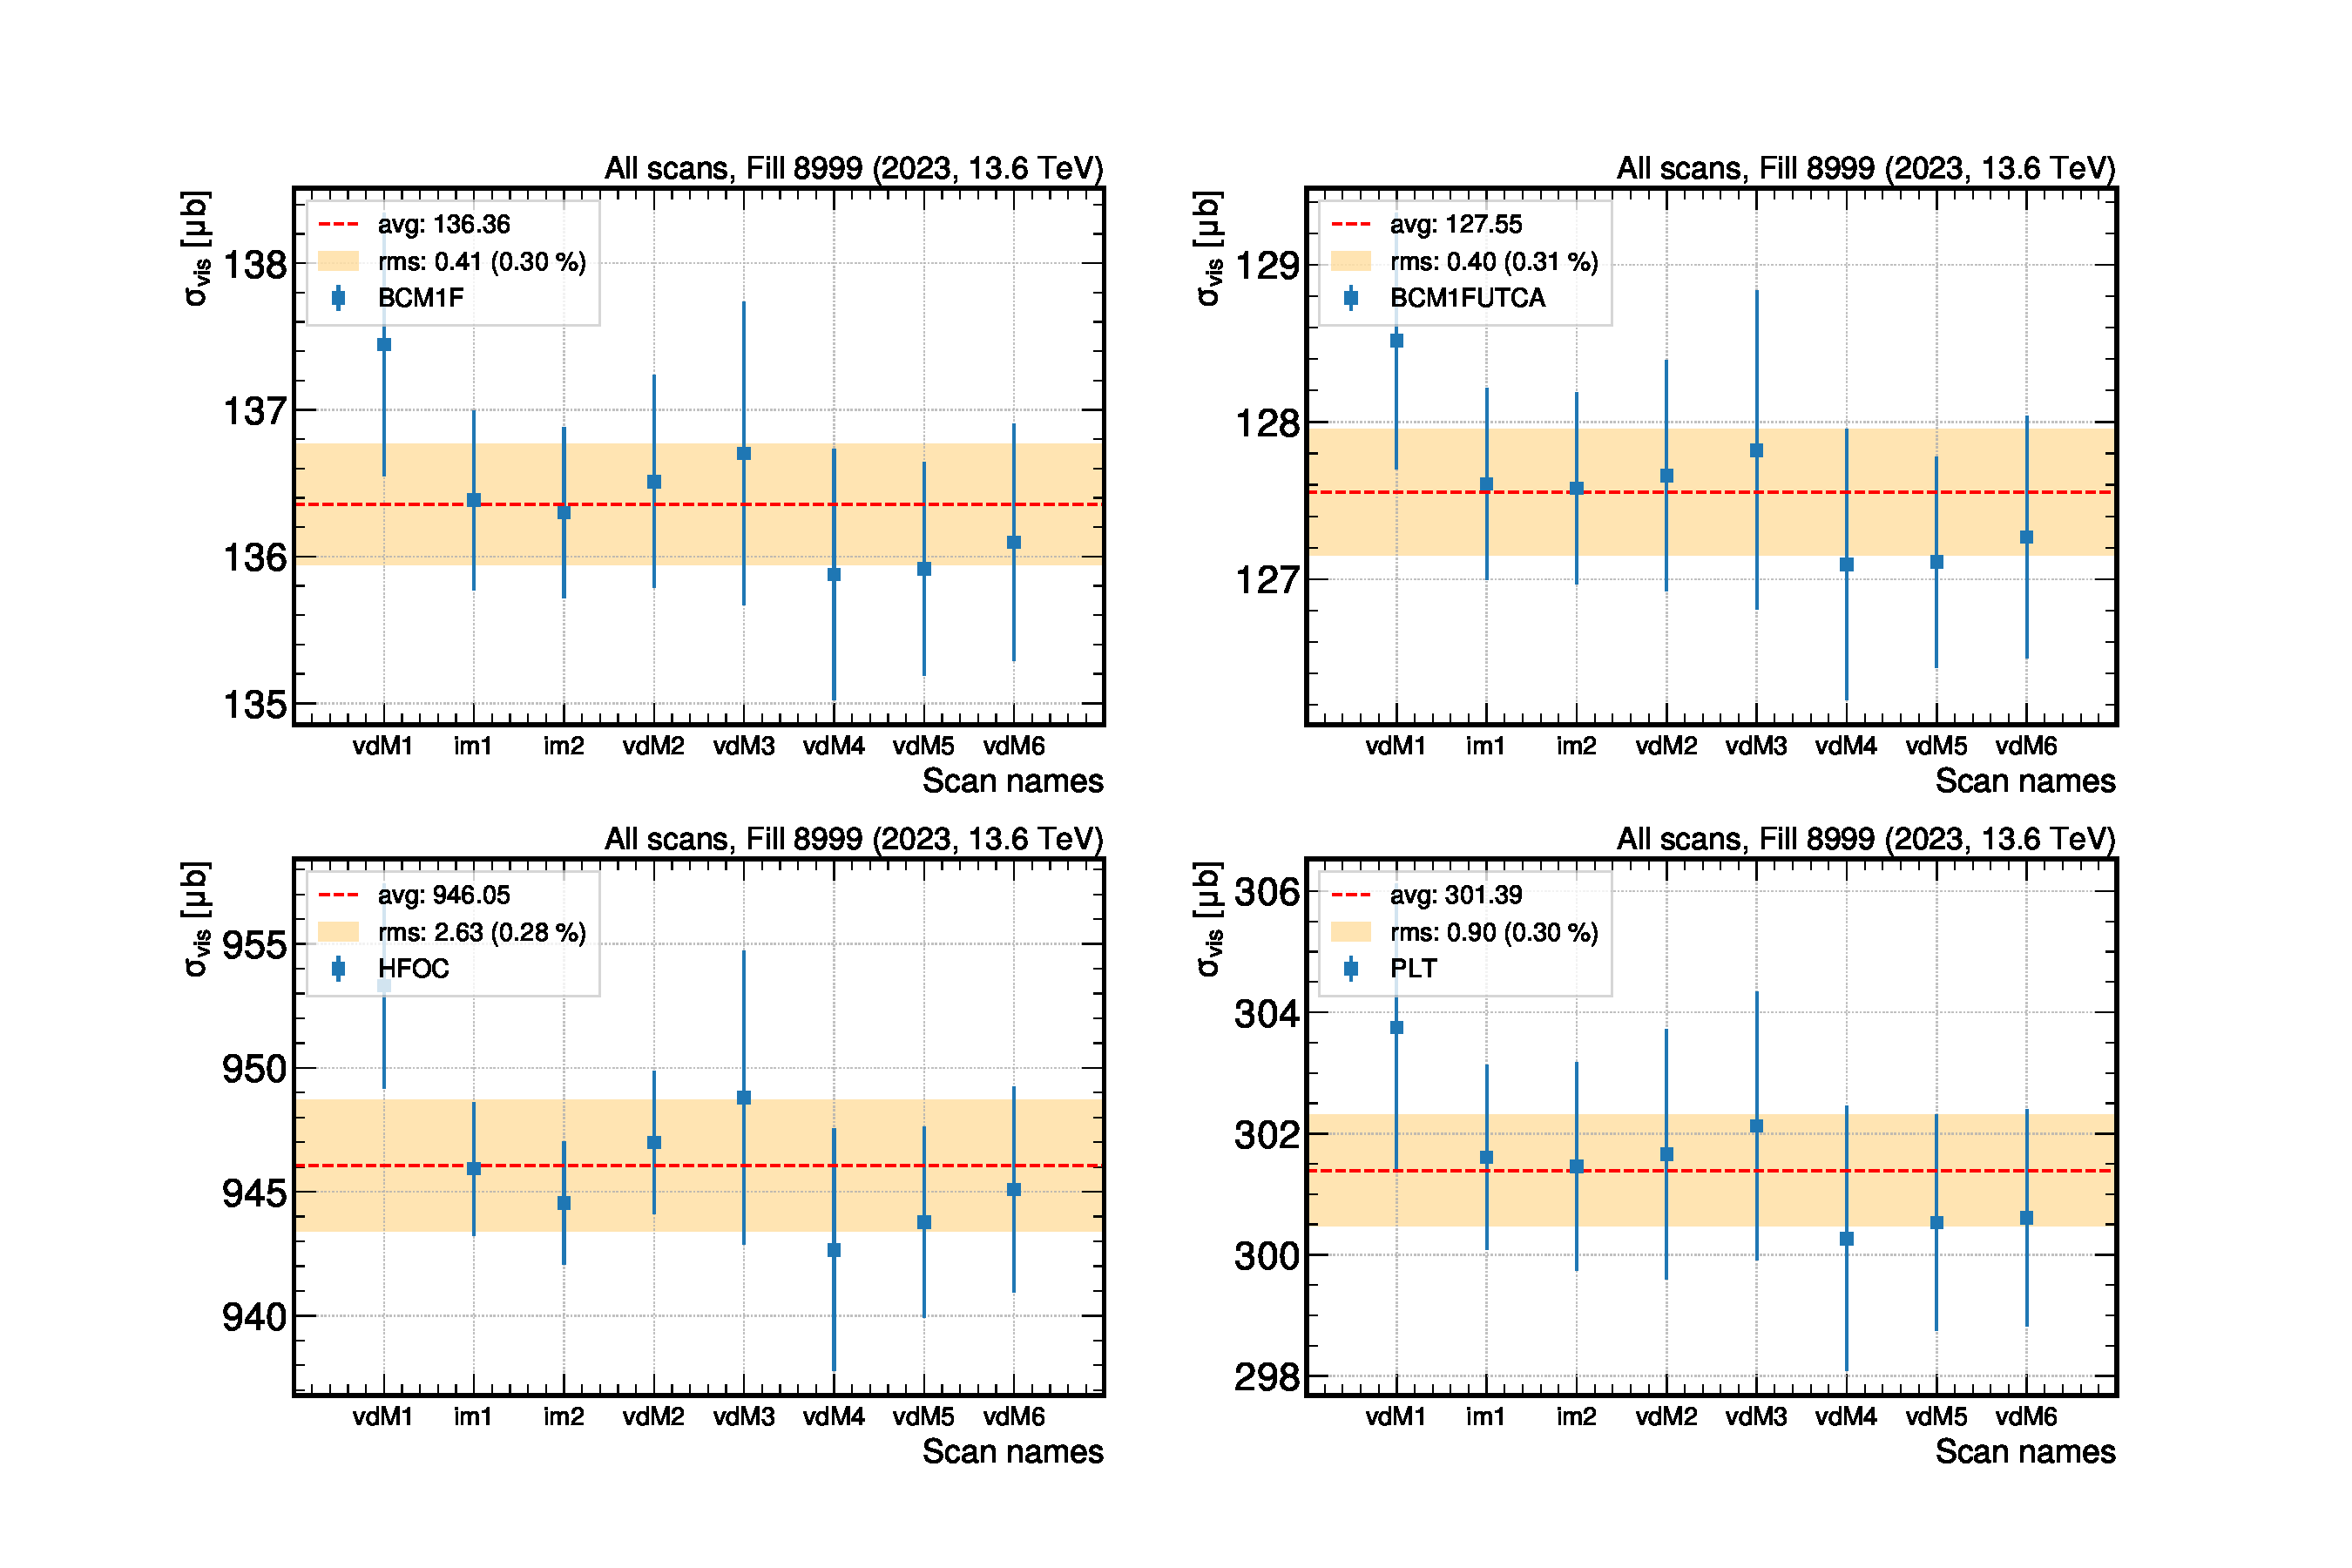
\includegraphics[width=0.7\paperwidth]{images/assets/all_Corr_luminometer_xsec.pdf}}
	\caption[Final visible cross section results for other online luminometers]{Final visible cross section results obtained after data corrections for BCM1F, BCM1FUTCA, HFOC and PLT luminometers.}
	\label{fig:all_Corr_luminometer_xsec}
\end{figure}

\begin{figure}[!htb]
	\centering
	\makebox[\textwidth]{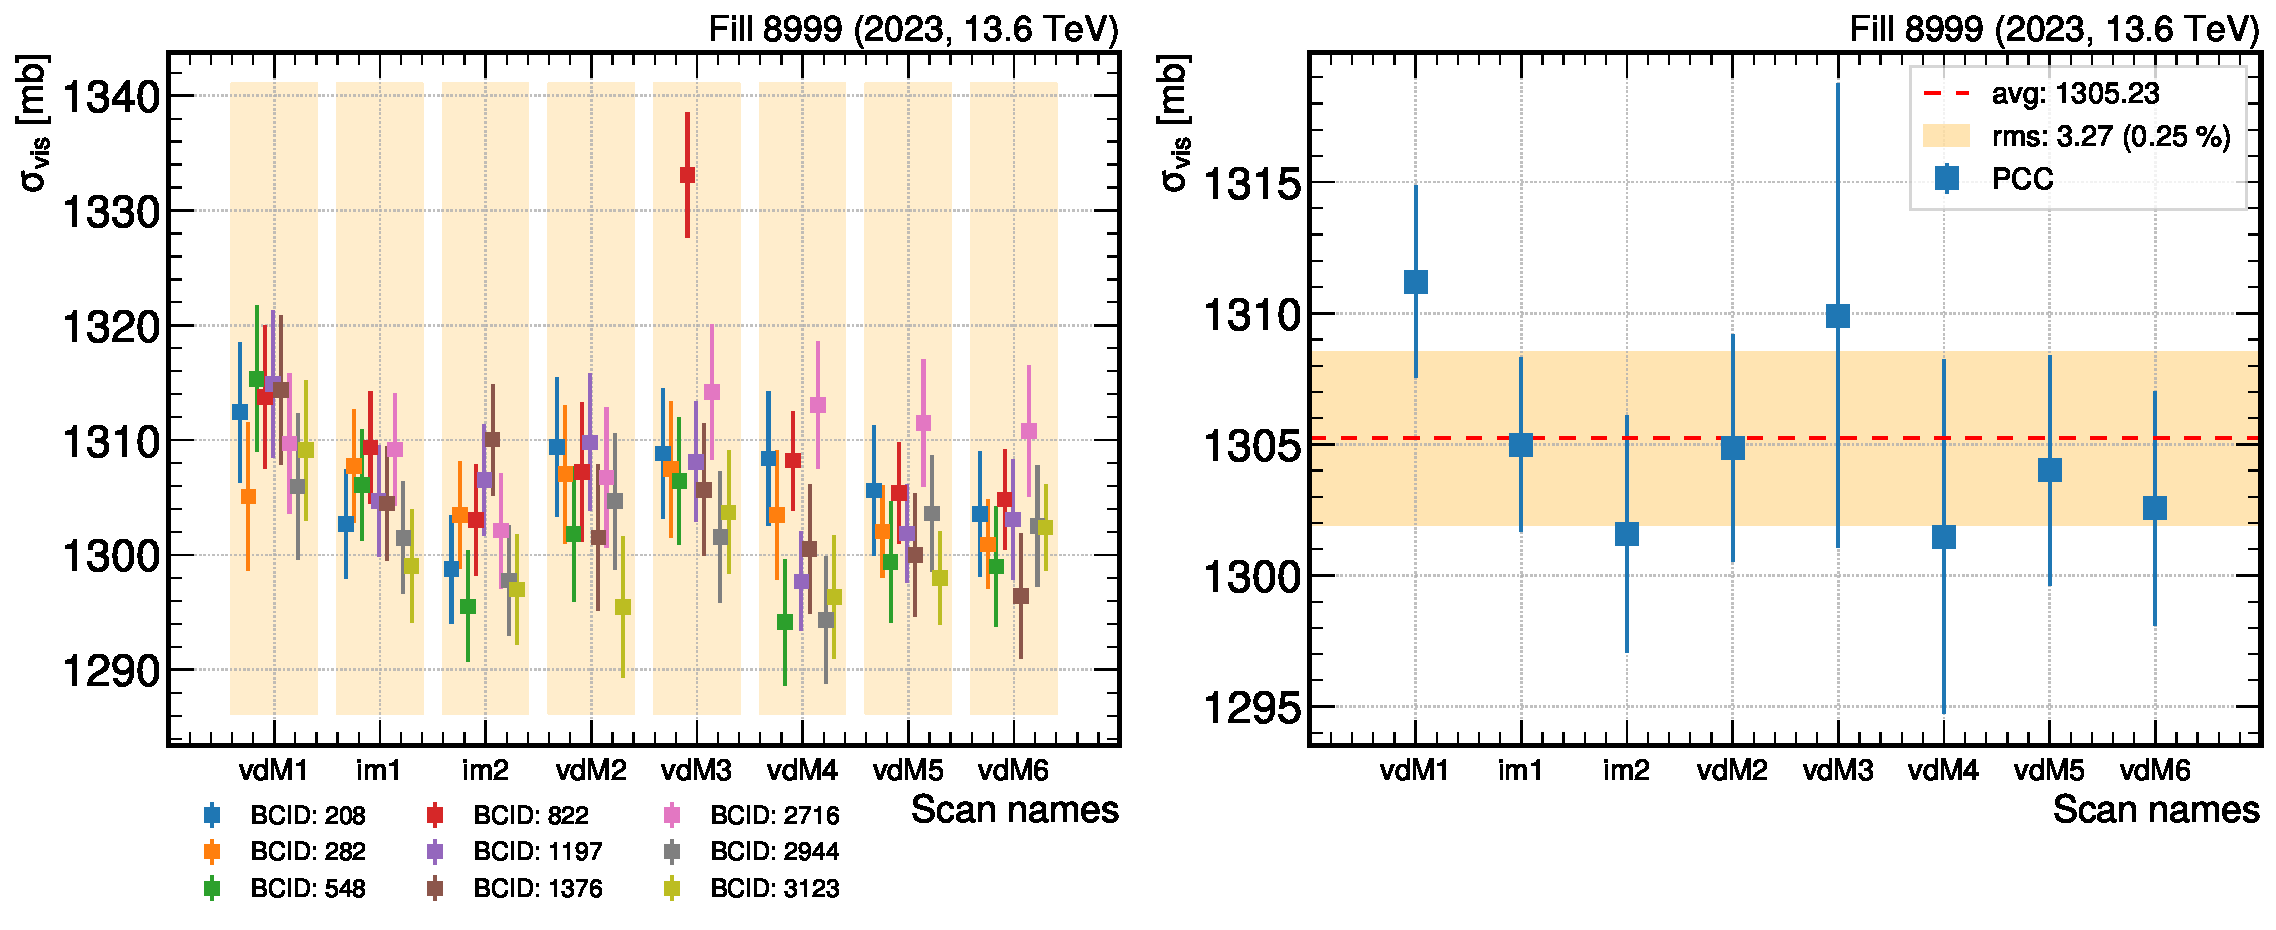
\includegraphics[width=0.6\paperwidth]{images/assets/cross_section_results_pcc.pdf}}
	\caption[PCC calibration results]{Left: PCC calibration results for all the vdM fill scans and recorded BCIDs (208, 282, 548, 822, 1197, 1376, 2716, 2944, and 3123). Right: PCC scan-to-scan variation across all vdM and im scans.
	}
	\label{fig:cross_section_results_pcc}
\end{figure}

The bunch-to-bunch variation in the visible cross section measurements is attributed as a source of uncertainty and has a magnitude of 0.6\%, the standard deviation of the mean in HFET. Similarly, the calibration variation across scans was also used as another source of uncertainty. HFET's weighted RMS across all scans, 0.28\%, was the attributed uncertainty.

The fit results were compared among the different luminometers and their individual reduced $\chi^2$ per scanning plane were plotted for all vdM scans. Overall, the results indicate good fit quality for both axis, with fits performed on HFOC reporting to have slightly higher reduced $\chi^2$ in the vertical plane. An example of the fits for the BCM1FUTCA detector is shown in \autoref{fig:fit_BCM1FUTCA_103} and the distributions for all online luminometers can be seen in \autoref{fig:chi2_distributions}.

\begin{figure}[!htb]
	\centering
	\makebox[\textwidth]{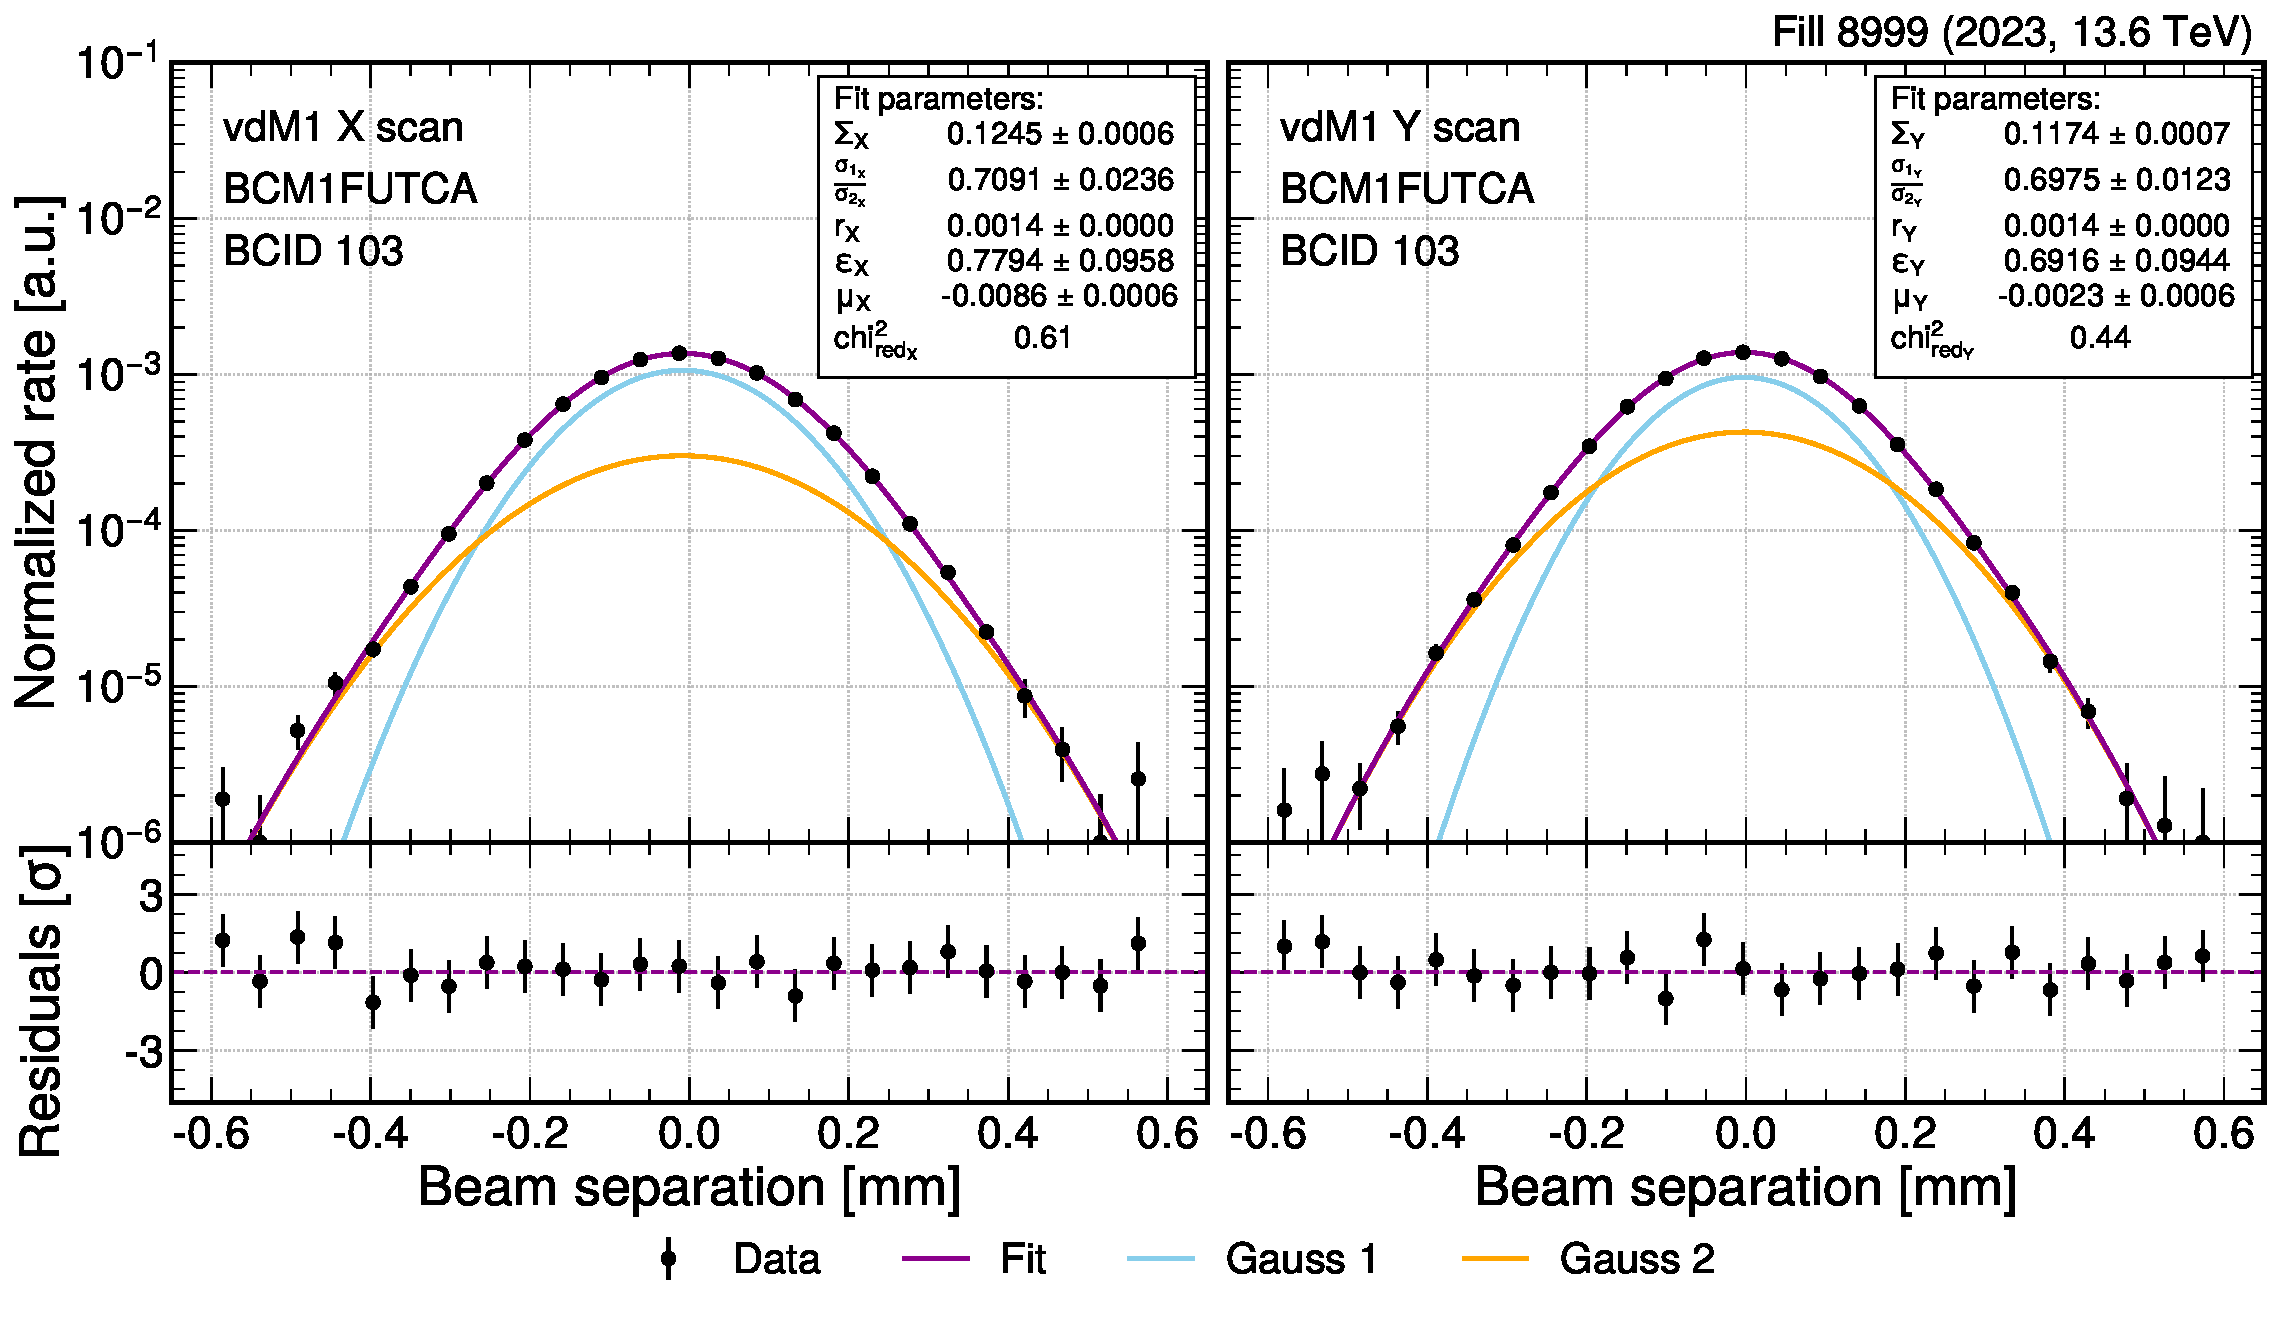
\includegraphics[width=0.7\paperwidth]{images/assets/fit_BCM1FUTCA_103.pdf}}
	\caption[Double Gaussian fits for BCM1FUTCA]{Double Gaussian fits to the BCM1FUTCA data recorded during the first vdM scan pair (vdM1), shown for the x (left) and y (right) scan. In the bottom panels, the statistical pull for each data point is shown. The boxes indicate the fit parameters for the fit in question. From top to bottom these contain the bunch overlap width, the ratio between both Gaussians, the rate at the peak, the weight factor for the first Gaussian curve, the mean of the overall distribution, and the reduced $\chi^2$.}
	\label{fig:fit_BCM1FUTCA_103}
\end{figure}

\begin{figure}[!htb]
	\centering
	\makebox[\textwidth]{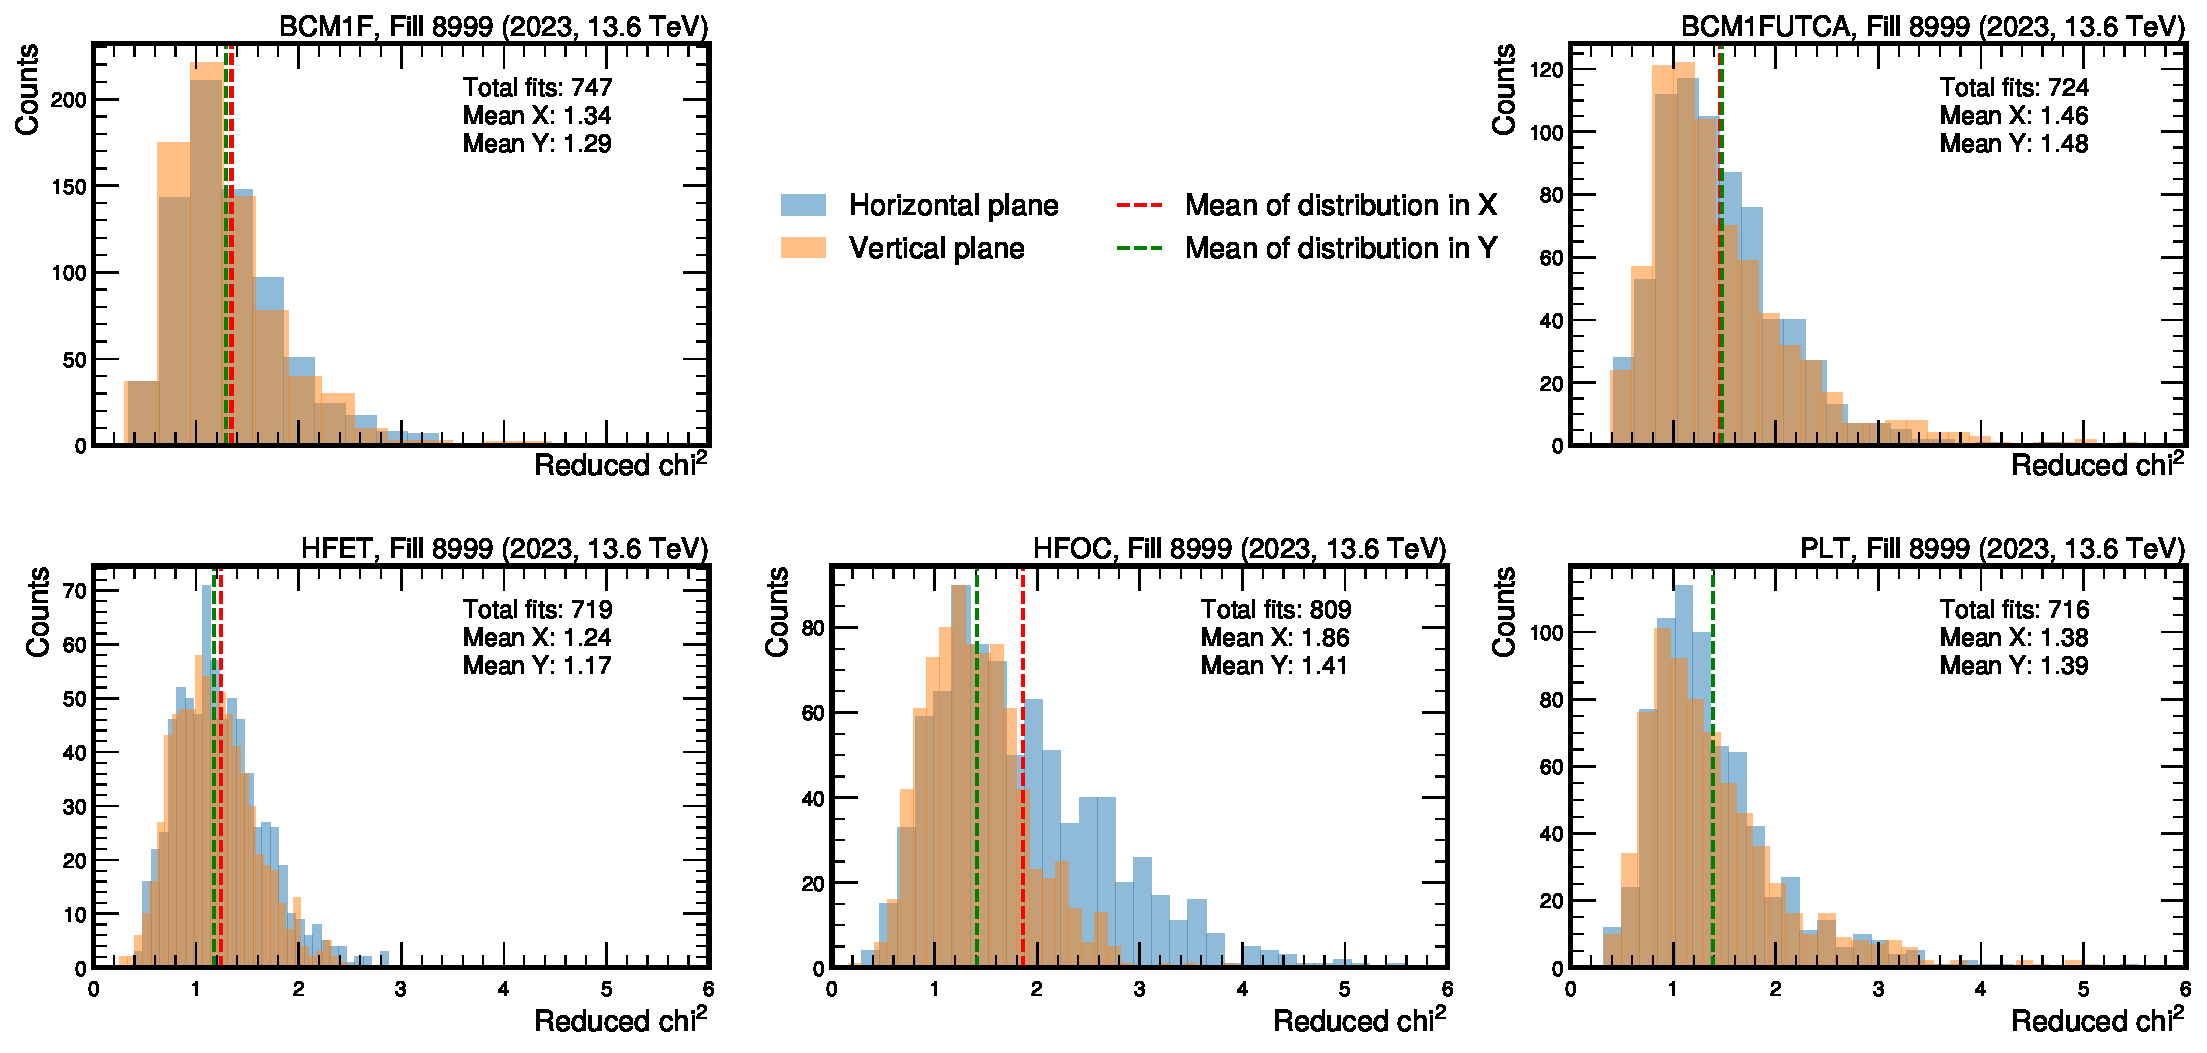
\includegraphics[width=0.7\paperwidth]{images/assets/chi2_distributions.pdf}}
	\caption[Scan fits reduced $\chi^2$ distribution]{Overview of the reduced $\chi^2$ distributions for all online luminometers for both scanning planes and all vdM scans. Only fits which converge are considered which leads to a slightly different total number of fits per detector.}
	\label{fig:chi2_distributions}
\end{figure}

Using the resulting fits, we extract the measured effective width and height of the luminous area, $\Sigma_X$ and $\Sigma_Y$, for all of the luminometers. As it is a property of each bunch-pair, determined by their emittances and the constant $\beta^{*}$ at CMS, it should be consistent for all luminometers. The comparison is shown in \autoref{fig:capsigma_vdm1} and \autoref{fig:capsigma_evol}, and good agreement is observed. In the latter figure, the time-evolution of beam emittances can be observed.

\begin{figure}[!htb]
	\centering
	\makebox[\textwidth]{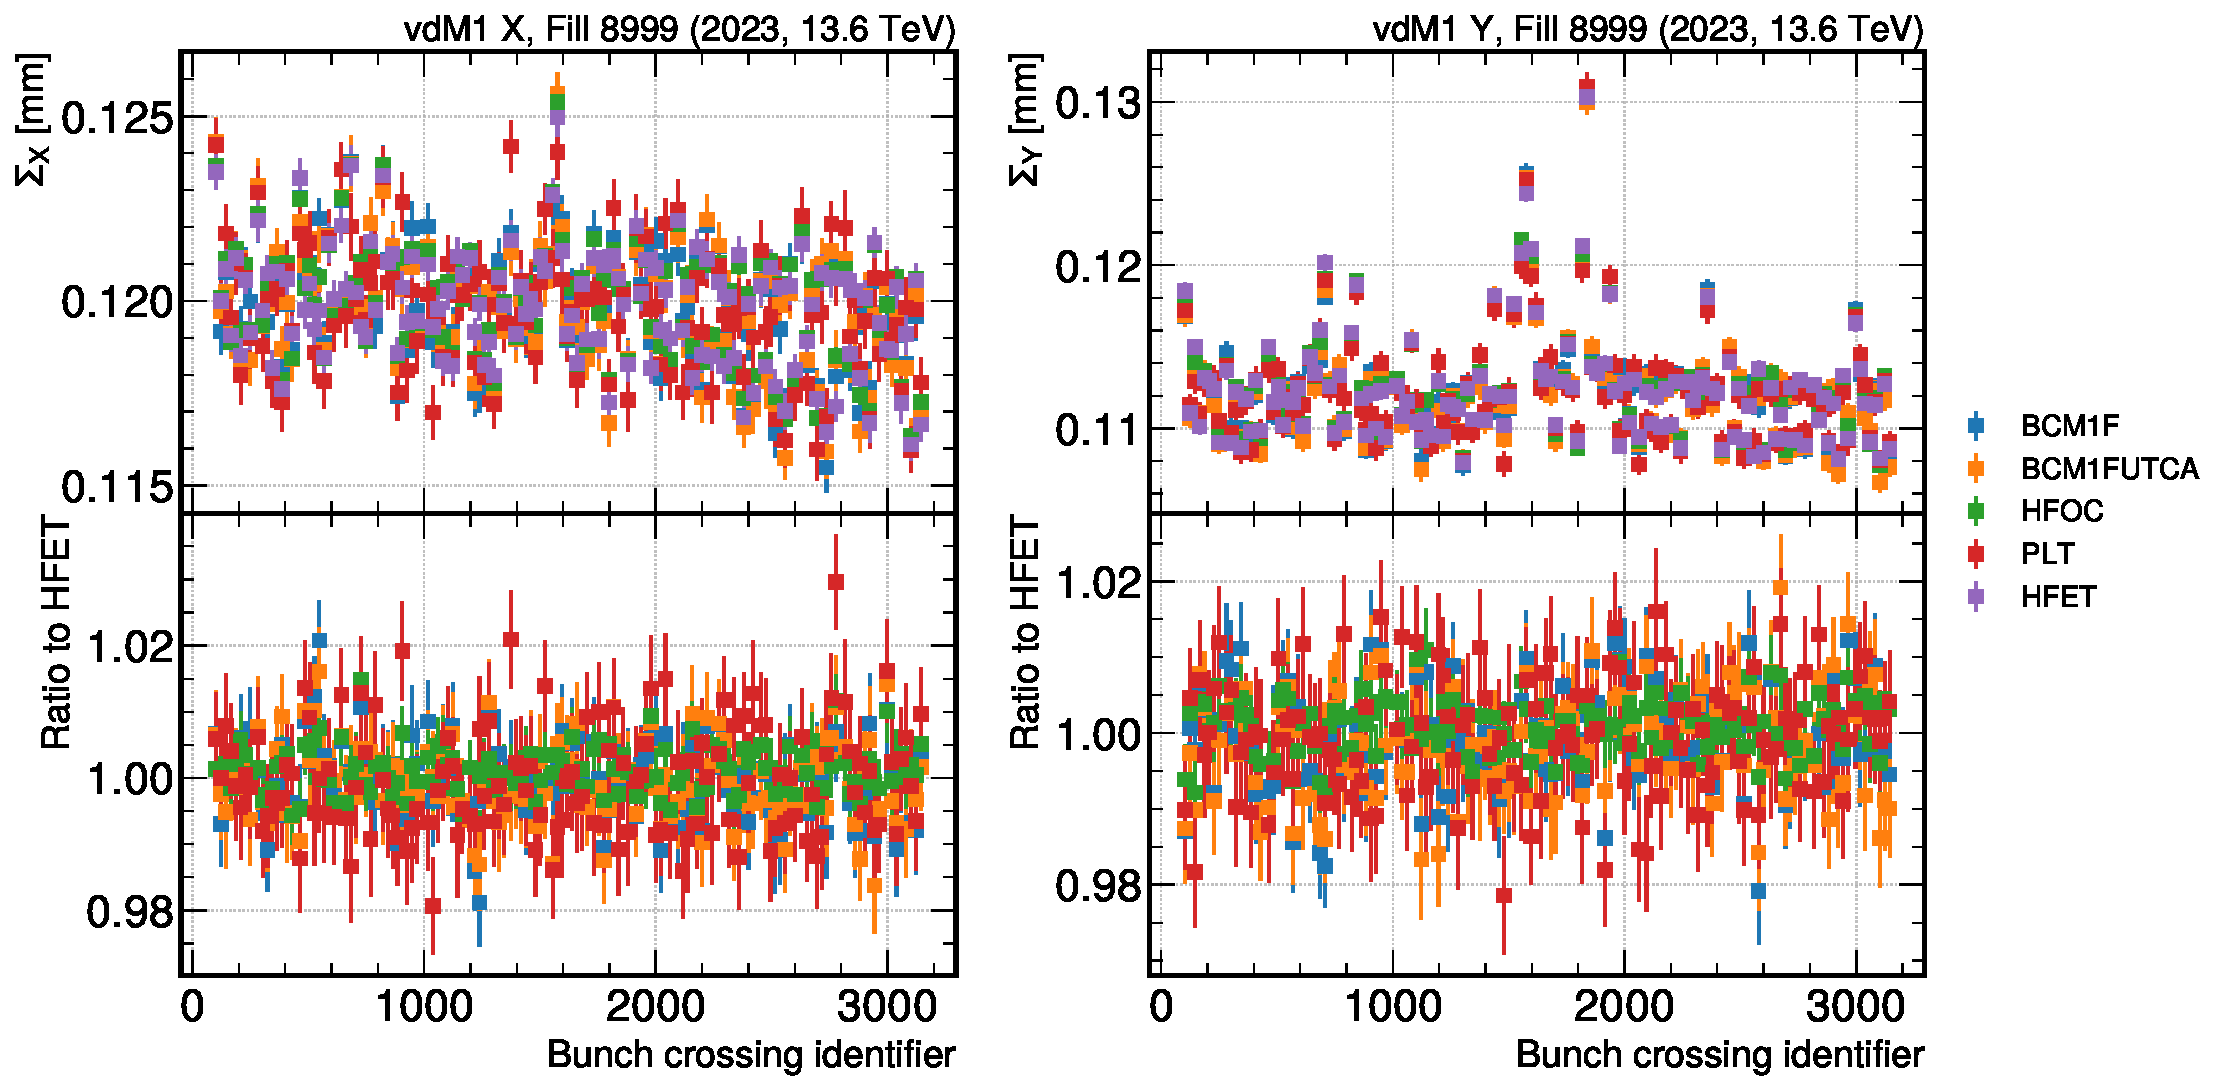
\includegraphics[width=0.6\paperwidth]{images/assets/capsigma_vdm1.pdf}}
	\caption[Overview of the measured effective beam overlap widths]{Overview of the effective width and height of the luminous area, $\Sigma_X$ and $\Sigma_Y$, measured during the vdM1 scan pair, by all the online luminometers (upper row). Ratios of the measured values by different systems with respect to HFET are also shown (bottom row).}
	\label{fig:capsigma_vdm1}
\end{figure}

\begin{figure}[!htb]
	\centering
	\makebox[\textwidth]{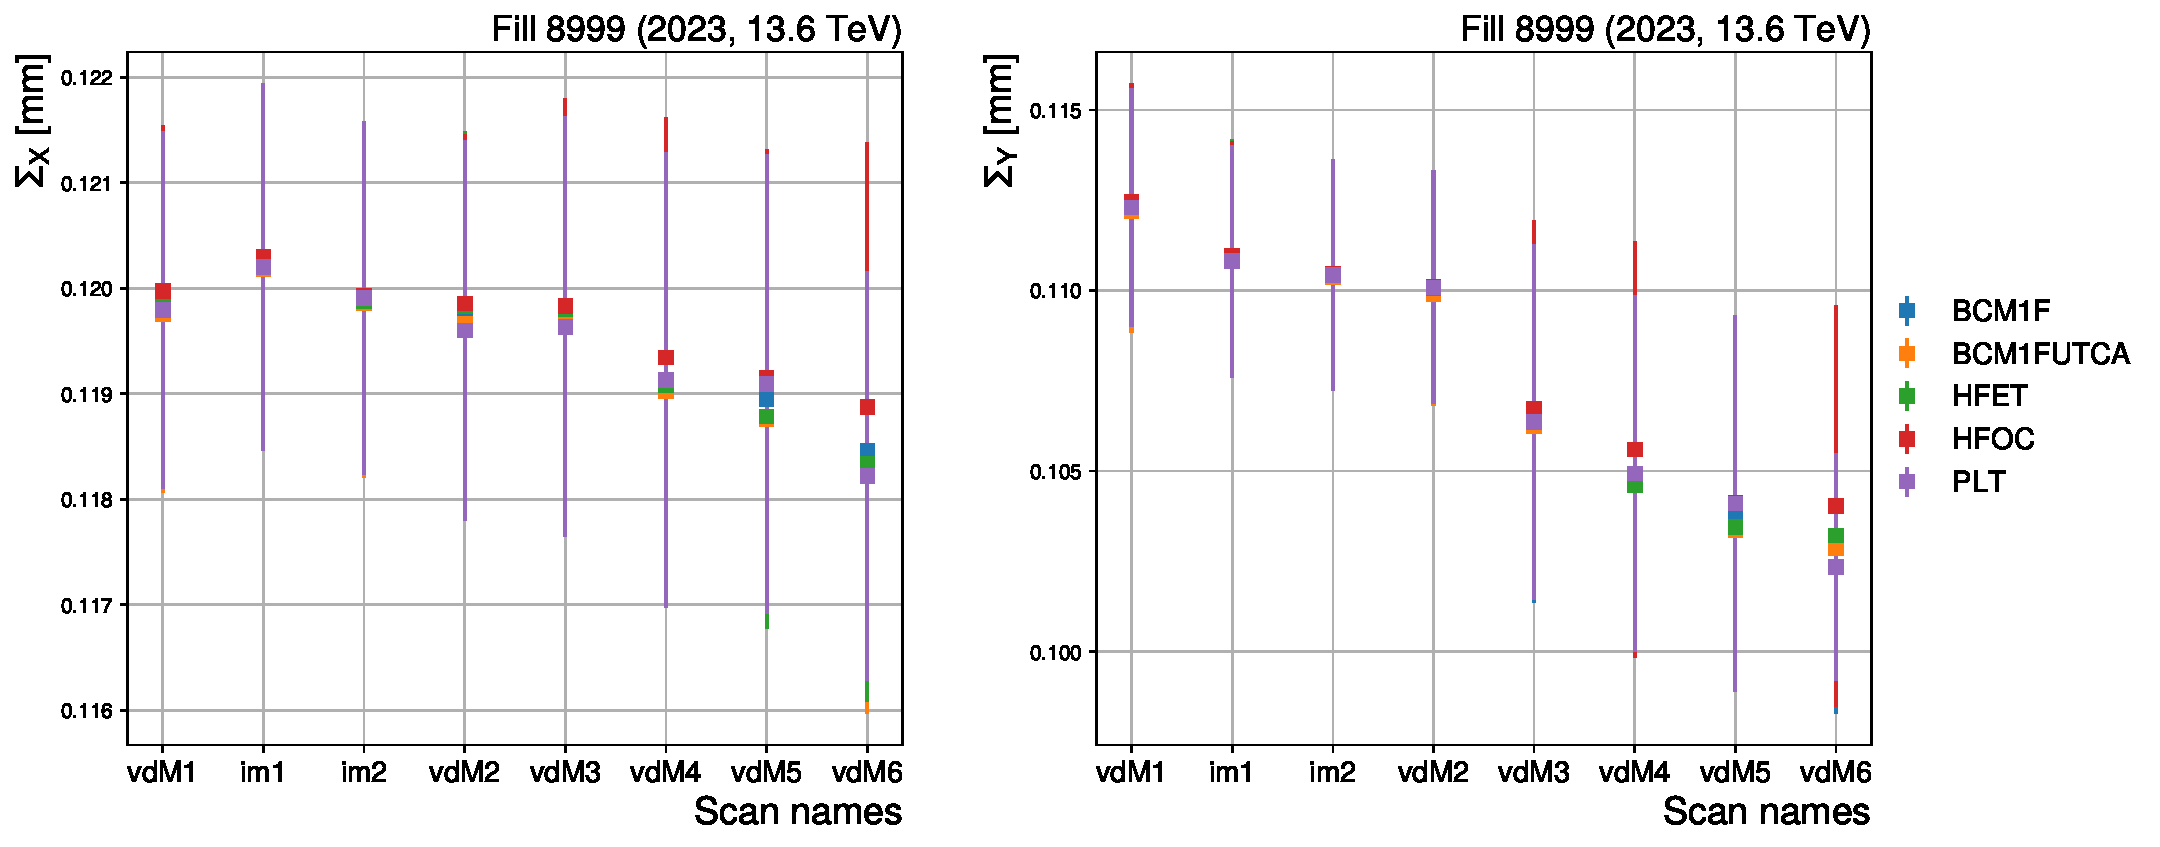
\includegraphics[width=0.6\paperwidth]{images/assets/capsigma_evol.pdf}}
	\caption{Overview of the average $\Sigma$ values in both transverse plans measured during all vdM and im scans, by all the online luminometers.}
	\label{fig:capsigma_evol}
\end{figure}

\newpage

\section{Integration}

In the previous section, the process by which the detector calibration factors were obtained was discussed. In this section, the performance of these calibrations in maximizing the agreement between luminometers during the vdM fill and, more importantly, under physics conditions is evaluated. A discussion on the year-long detector consistency will be presented, along with details on the specific stability corrections applied to the BCM1F. Additionally, the issue of detector non-linearity will be addressed, focusing on the PLT corrections. Finally, this section will present the final integrated luminosity for 2023, along with the associated relative uncertainty.

\newpage

\subsection{vdM Consistency}
\label{subsec:vdm_consistency}

Using the calibration values shown in \autoref{tab:xsec_summary}, the measured luminosity of each independently calibrated detector can be compared to visualize the detector agreement under vdM conditions. \autoref{fig:vdm_instantaneous_lumi_vs_time} shows the instantaneous luminosity throughout the entire vdM program.

\begin{figure}[!htb]
	\centering
	\makebox[\textwidth]{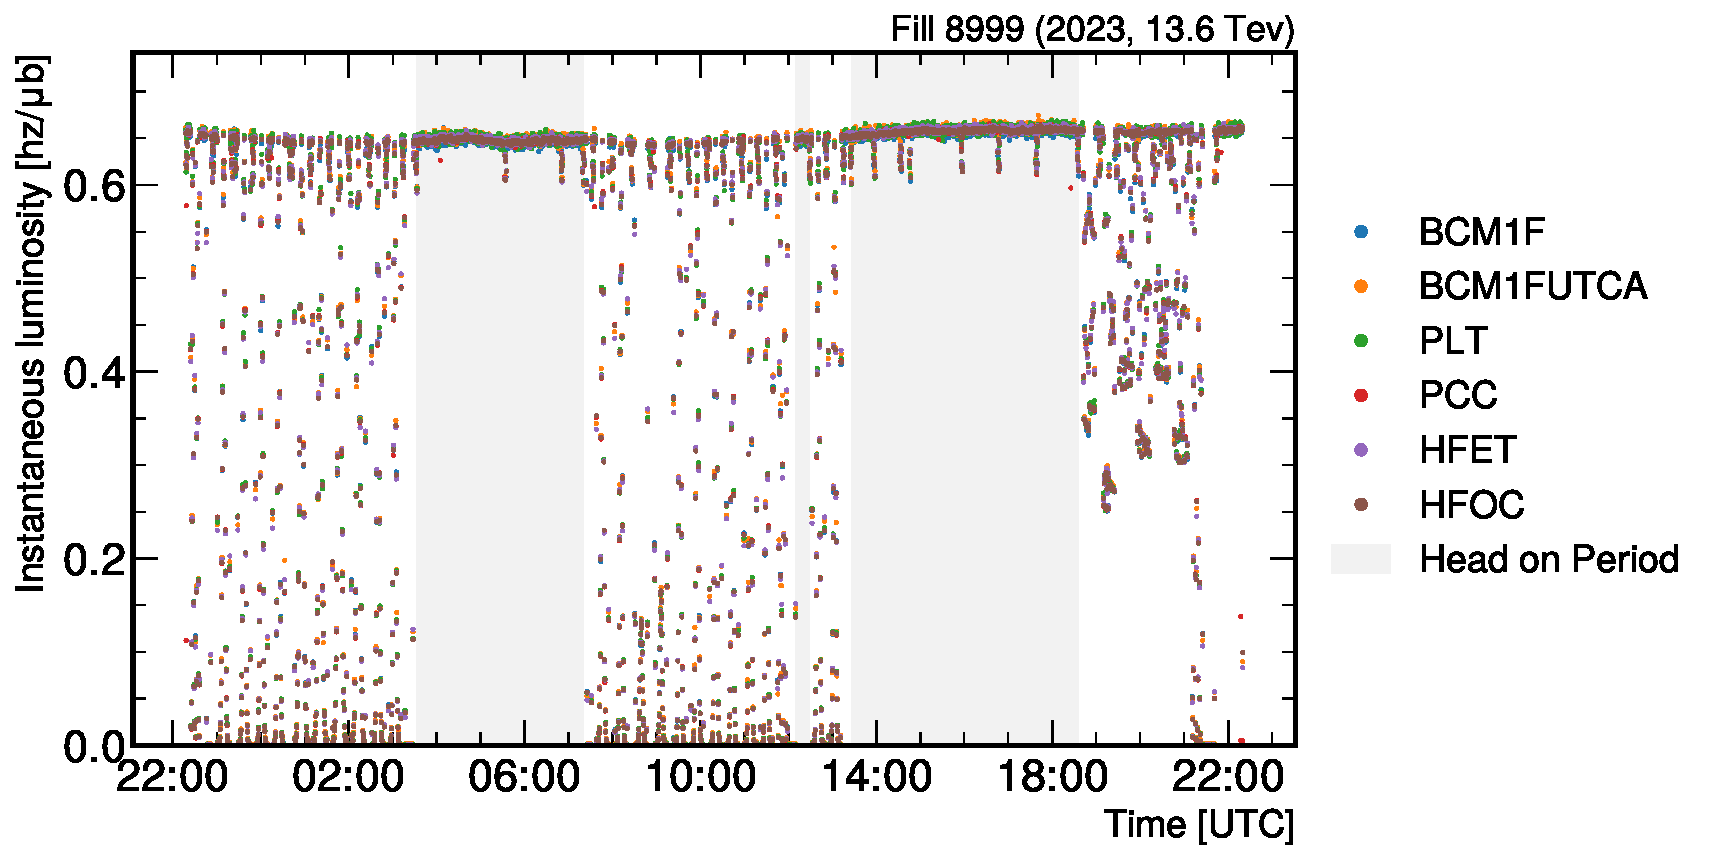
\includegraphics[width=0.6\paperwidth]{images/assets/vdm_instantaneous_lumi_vs_time.pdf}}
	\caption[Instantaneous luminosity during vdM]{Measured instantaneous luminosity as a function of time during the vdM program. All independently-calibrated luminometers show good agreement, especially during the head-on periods marked by the light grey areas.}
	\label{fig:vdm_instantaneous_lumi_vs_time}
\end{figure}

The luminometers show very good agreement with each other. The cross-detector consistency during the vdM fill was evaluated from the head-on ratios of all the luminometers with respect to the overall average. \autoref{fig:vdm_head_on_lumi_vs_time_and_ratio} shows the agreement of the luminometers during these periods in the vdM fill. The overall spread of the detectors was taken as the standard deviation of the means, with a magnitude of 0.16\% (see \autoref{fig:vdm_ratio_histograms}).

\begin{figure}[!htb]
	\centering
	\makebox[\textwidth]{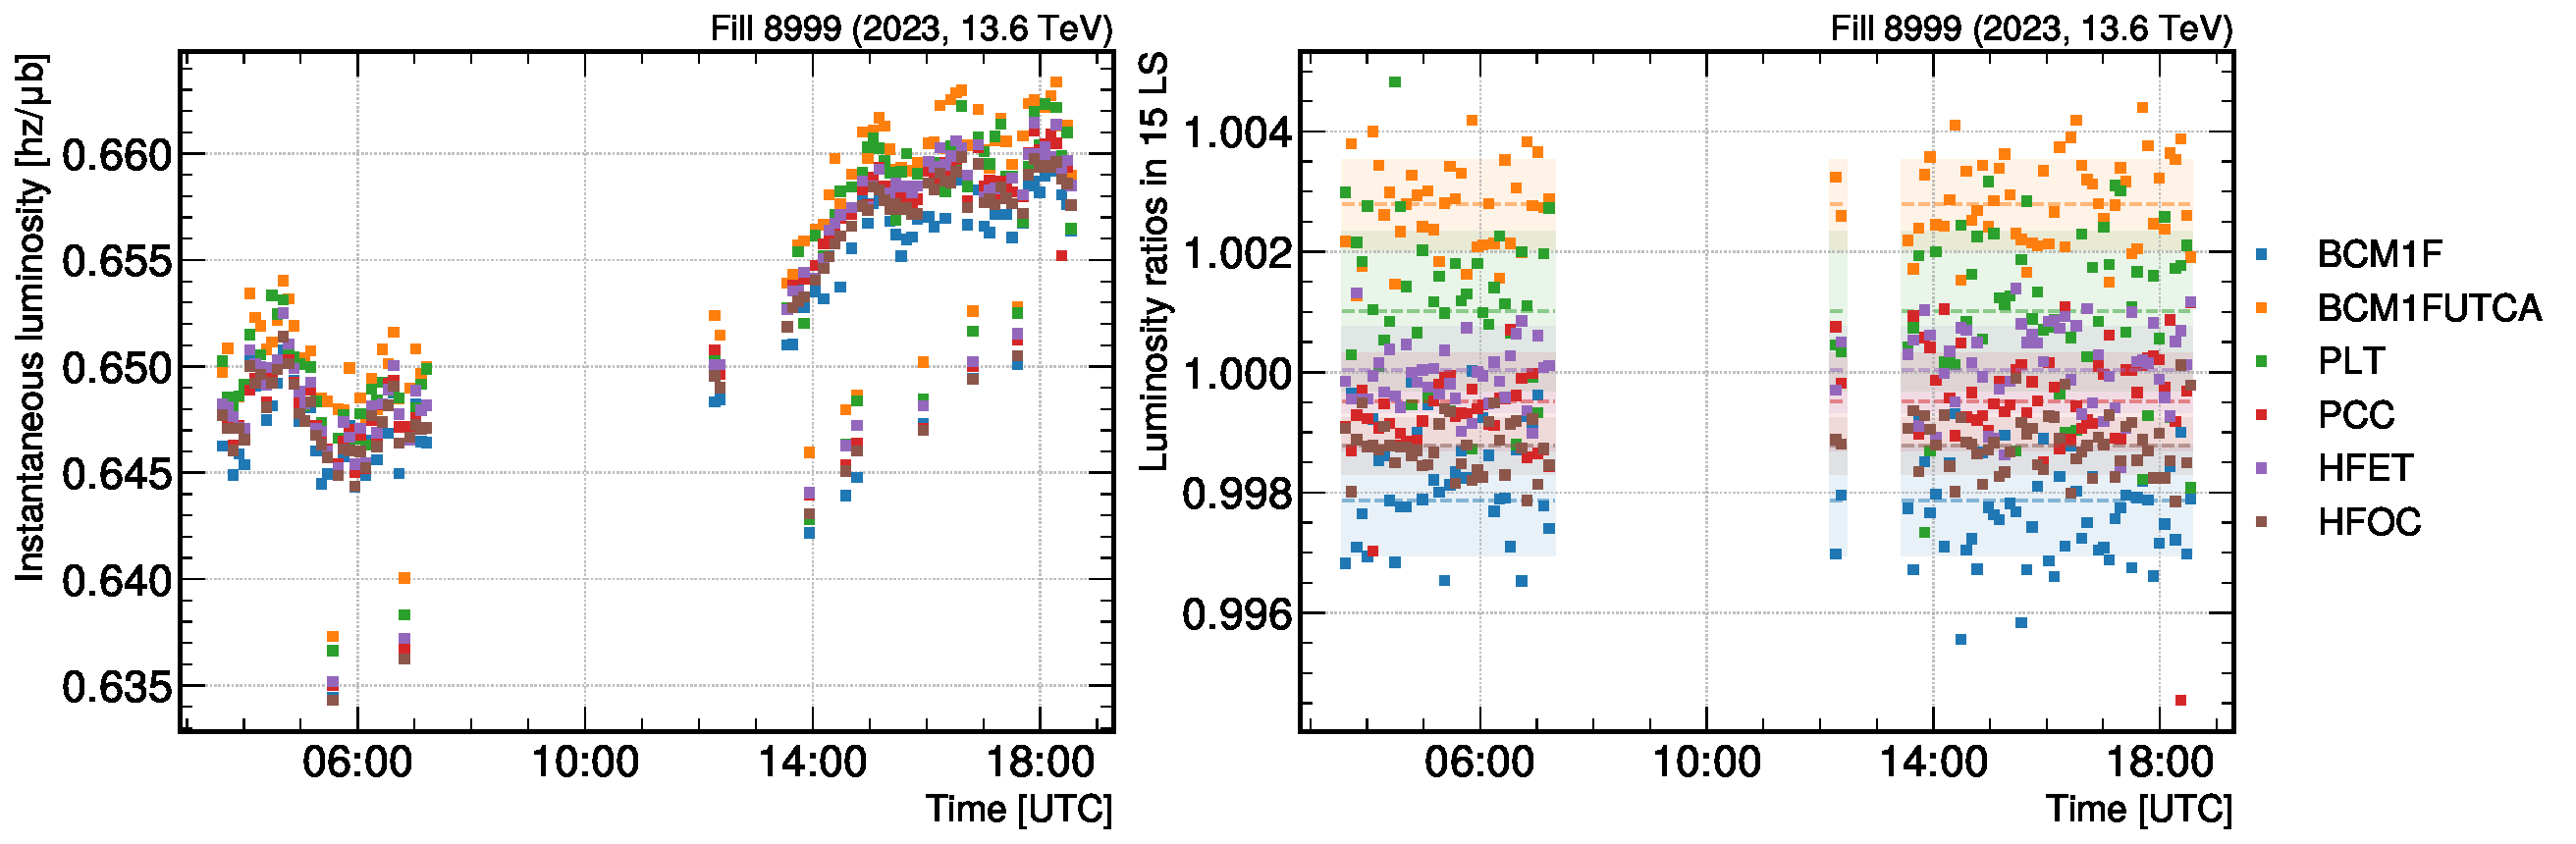
\includegraphics[width=0.7\paperwidth]{images/assets/vdm_head_on_lumi_vs_time_and_ratio.pdf}}
	\caption[Comparison of head-on luminosity measurements]{Head-on instantaneous luminosity measurements provided by the individual independently calibrated luminometers BCM1F, BCM1FUTCA, PLT, PCC, HFOC, and HFET during the LHC fill 8999 as a function of time. Each point corresponds to a time window of 15 lumisections, with each lumisection spanning about 23 seconds.}
	\label{fig:vdm_head_on_lumi_vs_time_and_ratio}
\end{figure}

The data in \autoref{fig:vdm_head_on_lumi_vs_time_and_ratio} corresponds to the periods when the LHC beams were colliding head-on, with all six luminometers taking high-quality data, and for the sum of the nine BCIDs for which PCC data was recorded in zero bias events. The ratio to the average measured luminosity is shown on the right and depicts an agreement well below 1\%. The statistical uncertainty associated with each point is found to be negligible and is not shown in the plot.

\begin{figure}[!htb]
	\centering
	\makebox[\textwidth]{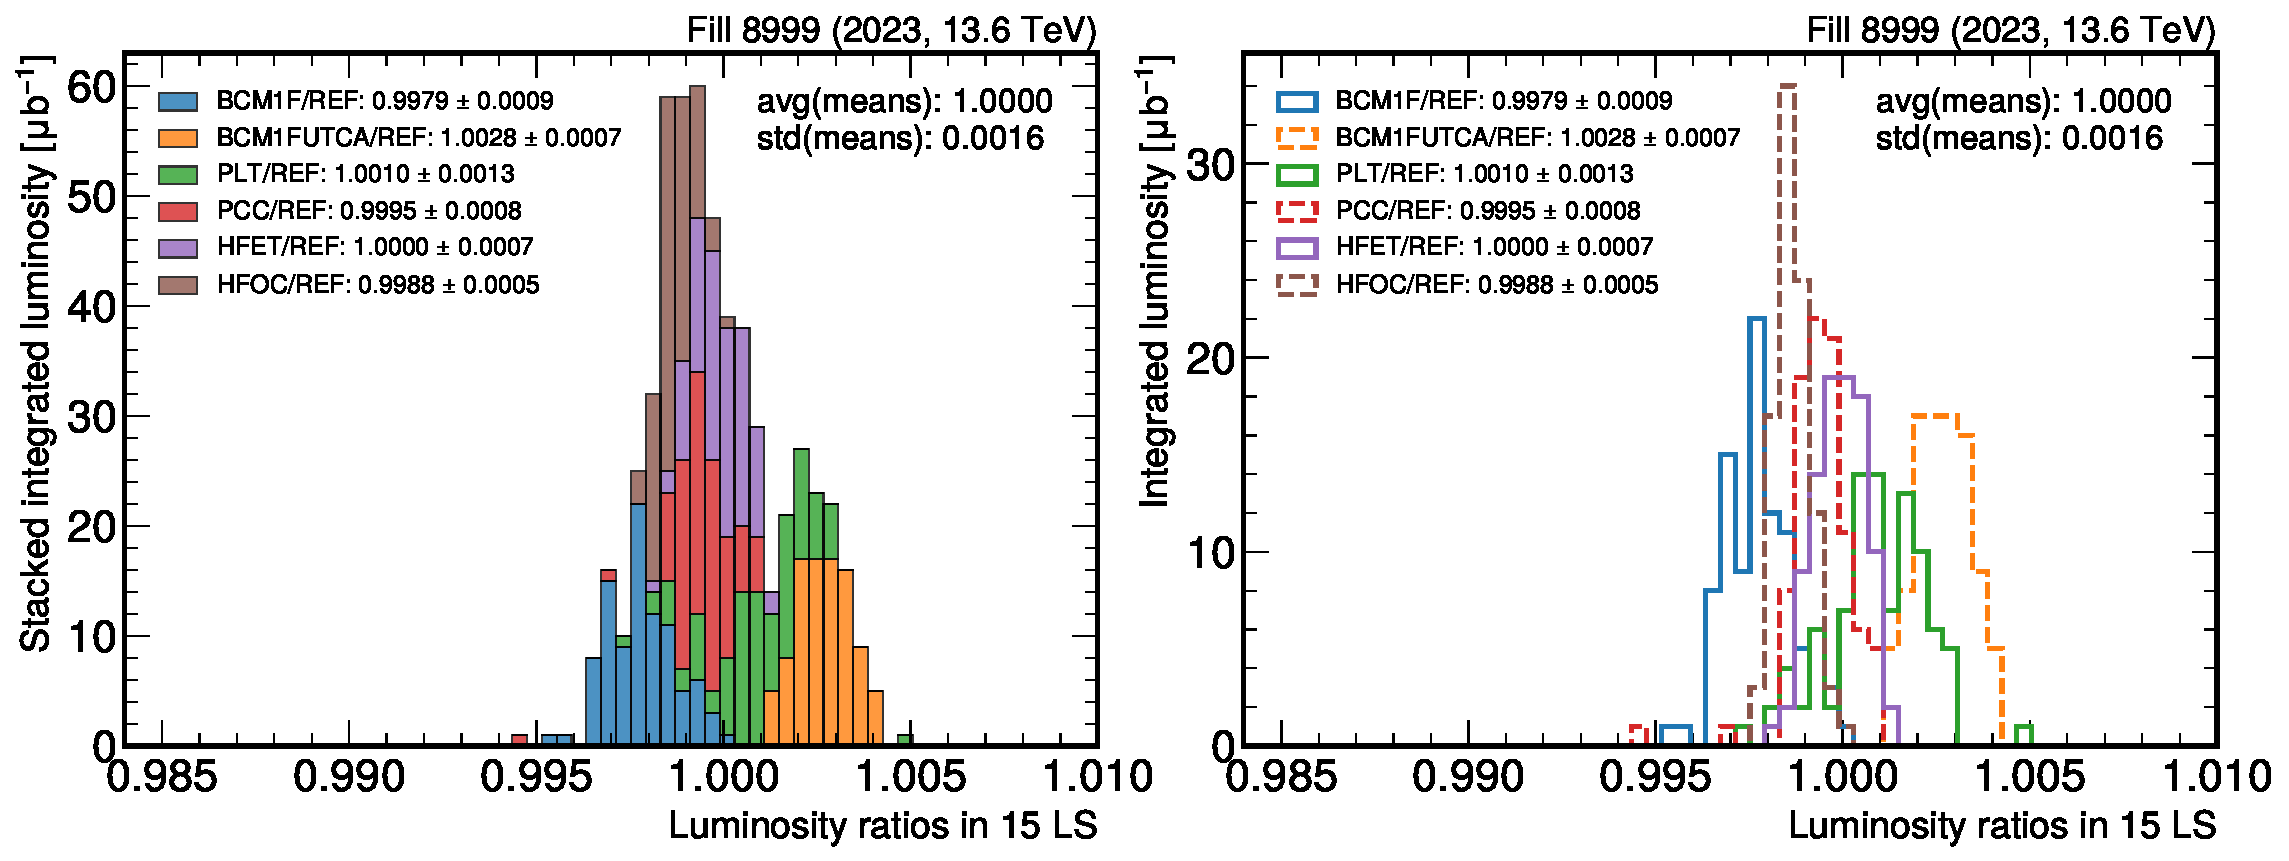
\includegraphics[width=0.7\paperwidth]{images/assets/vdm_ratio_histograms.pdf}}
	\caption[vdM luminosity ratio distributions]{Distributions of the ratio of the measured luminosities between different luminometers and the reference luminosity. The left plot shows a stacked distribution while the right plot shows individual distributions. The means and standard deviations of the individual distributions are shown. The reference luminosity (REF) corresponds to the average luminosity of all the individual luminometers.}
	\label{fig:vdm_ratio_histograms}
\end{figure}

With the vdM calibrations validated, they can be used to calibrate the rates of all luminometers for the entire running year in accordance with \autoref{eq:inst-luminosity}. The results of this calibration procedure are shown in \autoref{fig:vdm_only_year_stability}.

\begin{figure}[!htb]
	\centering
	\makebox[\textwidth]{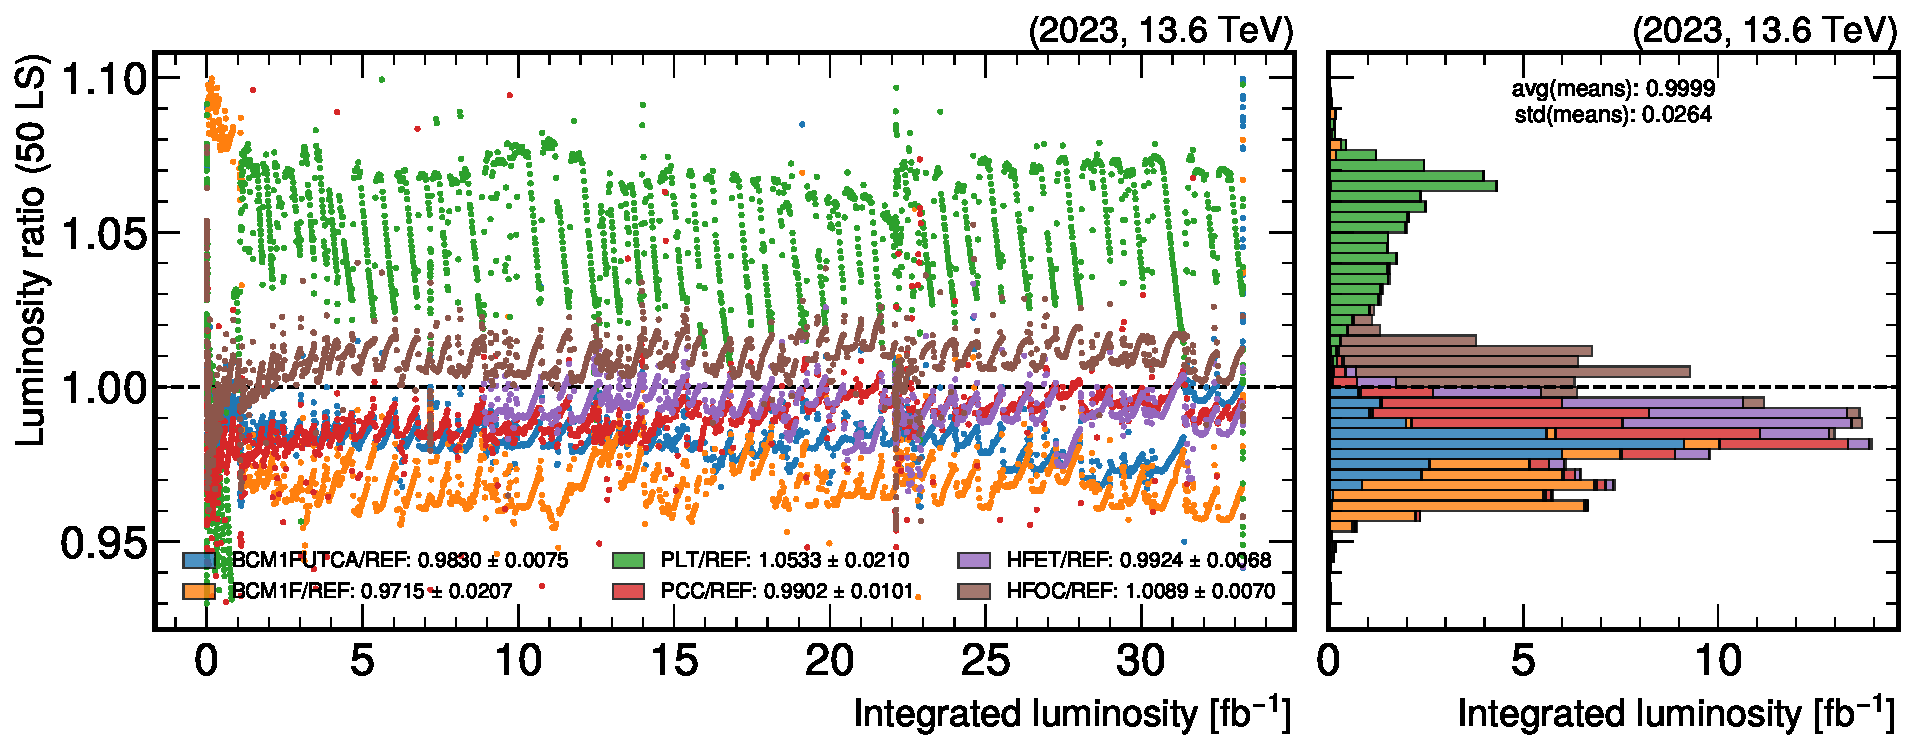
\includegraphics[width=0.7\paperwidth]{images/assets/vdm_only_year_stability.pdf}}
	\caption[Full year luminosity ratios with only vdM calibration]{The left plot shows the ratios of the luminosity measured in time windows of 50 LS (about 20 minutes) between the different luminometers and the average luminosity among them as a function of the integrated luminosity. The ratio distributions are shown in a histogram on the right, with the associated averages and standard deviations of the means indicated.}
	\label{fig:vdm_only_year_stability}
\end{figure}

Three main observations can be made when analyzing the ratios in \autoref{fig:vdm_only_year_stability}. The most obvious is the high discrepancy between different luminometers. PLT stands out as a clear example of this, but in general, the luminometers do not show good agreement. Secondly, some detectors exhibit significant steps throughout the year. Notable examples include BCM1F at the beginning and HFET from \(20.5 \, \text{fb}^{-1}\) to \(22 \, \text{fb}^{-1}\) and from \(27 \, \text{fb}^{-1}\) to \(27.5 \, \text{fb}^{-1}\). Lastly, the ratios show some non-linear responses, as is clearly seen in PLT. These observations highlight the difficulty in extrapolating the calibrations outside the vdM fill, as explained in \autoref{subsec:extrapolation_of_vdM_calibration}.

In the next sections, the issues of detector stability and non-linearity will be addressed, with examples of these corrections for the BCM1F and PLT detectors.

\subsection{Detector Stability}

The loss of efficiency that a detector exhibits throughout the year is corrected empirically by multiplying the detector's visible cross section by a factor \(\epsilon\), as explained in \autoref{eq:luminosity_integration}. The method for obtaining these factors is detailed below.

Many fills conducted during the year 2023 had designated beam time to perform emittance scans. From these scans, the detectors' visible cross sections are continuously measured, allowing for the tracking of the detectors' efficiency throughout the year. The loss of efficiency experienced by a detector is indicated by gradually decreasing \(\sigma_{\mathrm{vis}}\) measurements. When subsequent measurements do not follow the expected trend, it typically indicates that the detector is operating under non-optimized conditions. In such cases, the detector's running configurations are adjusted to restore normal operation conditions.

When extrapolating the vdM calibration to other fills, a linear regression is performed on the FOM values as a function of integrated luminosity. The fitted line is then normalized to the vdM since this represents our best calibration measurement. \autoref{fig:efficiency_bcm1f_example} shows the fit performed for the BCM1F measurements. The significant step at the beginning of \autoref{fig:efficiency_bcm1f_example} corresponds to a period when the BCM1F charge thresholds were set so high that it was counting noise as hits, leading to the apparent increase in efficiency.

\begin{figure}[!htb]
	\centering
	\makebox[\textwidth]{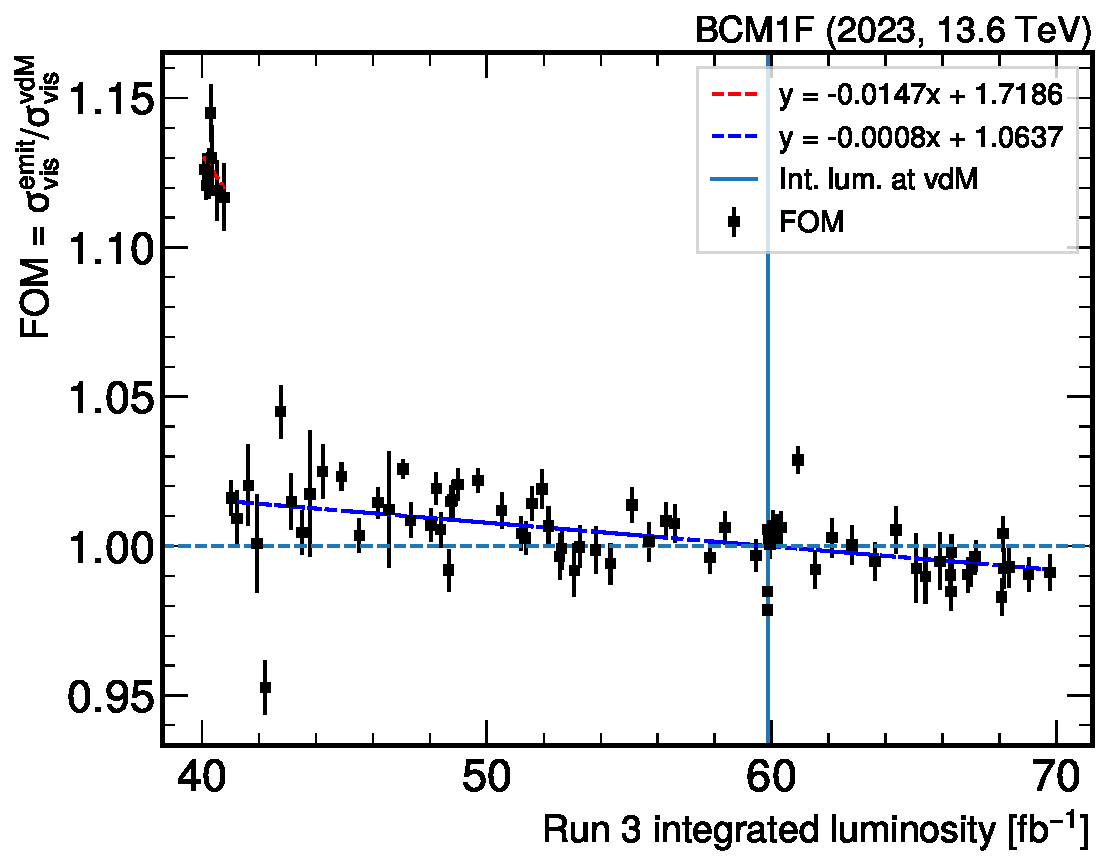
\includegraphics[width=0.5\paperwidth]{images/assets/efficiency_bcm1f_example.pdf}}
	\caption[BCM1F efficiency analysis results]{The results of emittance scan analysis for the BCM1F detector. The FOM values are shown as a function of integrated luminosity throughout Run 3. There are two distinct regions that are fitted independently, with the fit parameters shown in the legend.}
	\label{fig:efficiency_bcm1f_example}
\end{figure}

Once the fits are performed, the fit values at each point are used to extrapolate the vdM calibrations for the corresponding fills.

\subsection{Detector Non-Linearity}
\label{subsec:detector_non_linearity}

At the time of writing, non-linearity corrections were only carried out for BCM1F and PLT. As explained in \autoref{subsec:extrapolation_of_vdM_calibration} a detector assumed to have a good linear response to varying experimental conditions is used as the reference for which other detectors will be corrected for. In this analysis the DT luminometer, referenced in \autoref{subsec:dt}, will be used as the reference assumed to be linear.

As in the previous section, this correction is also done at the fill level. However, in order to minimize the correlation between the luminosity of the detectors to the reference detector, only a small number of fills with a large SBIL range are considered. The linearity correction for PLT is detailed below.

A total of 10 fills, spread across the year, were chosen to determine the slope quantifying the amount of non-linearity. For each fill, the luminosity ratios with respect to DT as a function of SBIL were computed. The fills before and after the vdM fill were placed in different groups since PLT's running configurations were changed in order to improve its efficiency for the vdM fill. The results of this analysis are shown in \autoref{fig:plt_dt_relative_non_linearity}.

\begin{figure}[!htb]
	\centering
	\makebox[\textwidth]{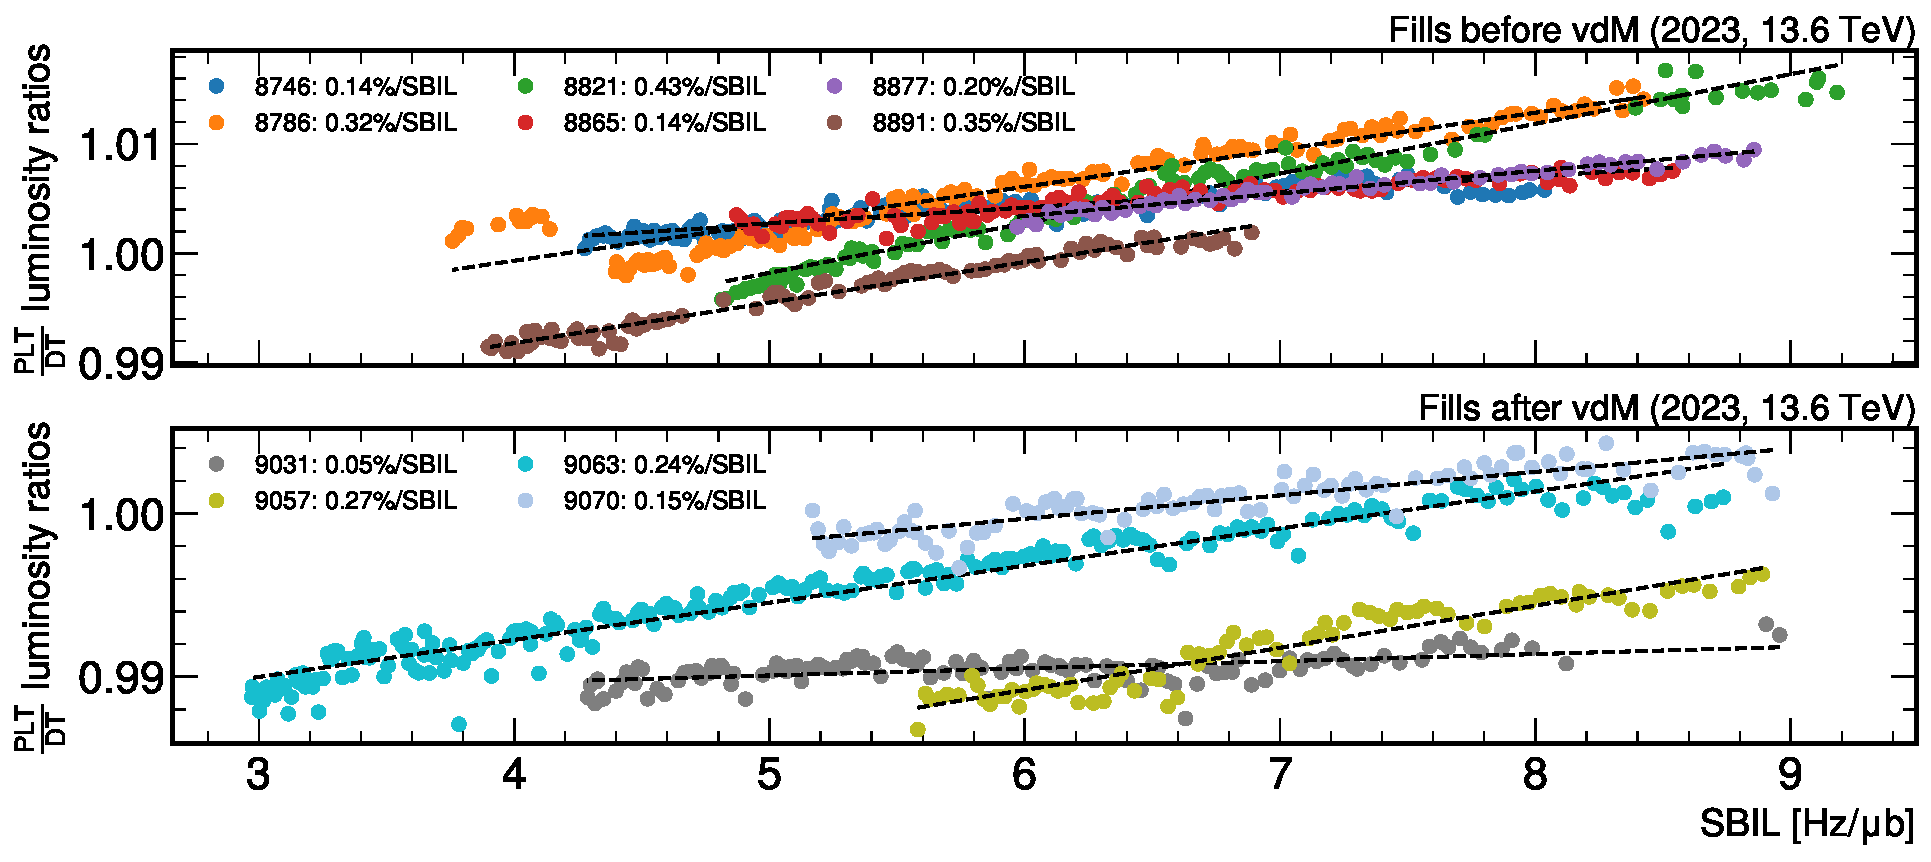
\includegraphics[width=0.7\paperwidth]{images/assets/plt_dt_relative_non_linearity.pdf}}
	\caption[PLT relative non-linearity slopes]{PLT non-linearity slopes extracted using DT as the reference luminometer for selected fills. The dashed lines correspond to the linear fits and the slopes are shown in \% per SBIL in the legend. The upper plot contains the fills before the vdM program and the bottom plot contains the fills after.}
	\label{fig:plt_dt_relative_non_linearity}
\end{figure}

The extracted slopes have to by $1\%/\text{SBIL}$ since this was the non-linearity configuration assumed during online data taking. Averaging the 2 regions yielding $1.06\%/\text{SBIL}$ and $0.98\%/\text{SBIL}$ for before and after vdM, respectively. 

For BCM1F, the non-linearity was extracted from a $\mu$-scan fill. A $\mu$-scan is a vdM-like scan that also spans a much wider SBIL range. The slopes were extracted in the same way as in the 2022 analysis \cite{CMS-PAS-LUM-22-001} and a $-0.12\%/\text{SBIL}$ correction was applied.

\subsection{Establishing a Reference Detector}

In \autoref{fig:vdm_only_year_stability}, the ratios were taken with respect to the average luminosity of all luminometers. However, the luminosity results have to be available via the \textit{brilcalc} database, which places constraints on the data format. For this reason, at the time of writing, DT was chosen as the reference detector. Since DT is not a independently-calibrated luminometer due to lack of available statistics, it was calibrated to the average of the other luminometers, effectively representing the average luminosity among them.

During the 2023 analysis, DT had been cross-calibrated to HFET in fill 9036 which yielded an calibration of $\sigma^{\text{DT}}_{\mathrm{vis}} = 179725 \mu b$. To scale this cross-calibrated version of DT to the luminosity average, the average ratio of every other luminometer with respect to this DT was taken. The results are shown in \autoref{tab:dt_cross_calibration}.

\begin{table}[!htb]
	\caption{Average and RMS of all fully-corrected independently-calibrated luminometers with respect to HFET-cross-calibrated DT.}
	
	\label{tab:dt_cross_calibration}
	\centering
	\begin{tabular}{lcccc}
		\hline
		Luminometer & Average ratio to cross-calibrate DT & RMS \\
		\hline
		BCM1F     & 0.985 & 0.005 \\
		BCM1FUTCA & 0.985 & 0.005 \\
		HFET      & 0.998 & 0.005 \\
		HFOC      & 1.002 & 0.007 \\
		PLT       & 0.986 & 0.007 \\
		PCC       & 0.997 & 0.006 \\
		\hline
	\end{tabular}
\end{table}

Weighting the average of the values in \autoref{tab:dt_cross_calibration} by the inverse square of the individual RMS yields a corrective factor of 0.991. This final cross-calibrated version of DT is used as a reference for the stability and non-linearity uncertainties discussed in the following section.

\section{Final Luminosity Results}

As in \autoref{subsec:vdm_consistency}, the year-long detector stability is illustrated. The best visible cross sections are utilized, with stability and non-linearity corrections applied.

\begin{figure}[!htb]
    \centering
    \makebox[\textwidth]{\includegraphics[width=0.7\paperwidth]{images/assets/final_preliminary_year_stability.pdf}}
    \caption[Final full year stability]{The left plot shows the ratios of the luminosity measured in time windows of 50 LS (about 20 minutes) between different luminometers and the reference luminometer as a function of the integrated luminosity over the 2023 pp data-taking period.}
    \label{fig:final_preliminary_year_stability}
\end{figure}

A comparison of \autoref{fig:vdm_only_year_stability} and \autoref{fig:final_preliminary_year_stability} demonstrates a significant improvement in detector agreement. The standard deviation of the means decreased from $2.6\%$ to $0.71\%$, which corresponds to the uncertainty associated with the stability corrections.

\begin{figure}[!htb]
    \centering
    \makebox[\textwidth]{\includegraphics[width=0.7\paperwidth]{images/assets/year_slopes_final.pdf}}
    \caption[Residual relative non-linearity distributions]{Distributions of relative co-linearity slope values between different luminometers and the DT luminometer taken as reference (REF). Each histogram entry is weighted by the integrated luminosity of the fill.}
    \label{fig:year_slopes_final}
\end{figure}

To assign an uncertainty to any residual non-linearity in the detectors, the slopes are extracted for all fills, as explained in \autoref
{subsec:detector_non_linearity}. The resulting distributions are analyzed, as shown in \autoref{fig:year_slopes_final}.

The detector with the maximum deviation, HFET, is selected to assign the uncertainty for this step. HFOC is excluded due to its complex non-linearity effects, which were not corrected for. The value of $0.09\%/\text{SBIL}$ is multiplied by the average SBIL in 2023 of 6.6 H$z/\mu b$, resulting in an overall uncertainty of $0.59\%$.

Certain luminometers are unavailable for some periods throughout the year. Hence, all available luminometers are prioritized based on their measured luminosity contributions to the integrated luminosity. For this analysis, the priority order is DT, PCC, HFET, PLT, and BCM1FUTCA. The total delivered luminosity was 32.74 $\text{fb}^{-1}$, and the CMS recorded luminosity was 30.12 $\text{fb}^{-1}$, with an associated uncertainty of 1.28\%, as summarized in \autoref{tab:sum}.

\begin{table}[!h]
    \centering
    \caption{Summary of uncertainty contributions for the 2023 luminosity calibration analysis.}
    \label{tab:sum}
    \begin{tabular}{lc}
        \textbf{Source} & \textbf{Uncertainty} (\%) \\ \hline
        \textbf{Calibration} & \\
        Beam current & 0.20 \\
        Ghosts \& satellites & 0.10 \\
        Orbit drift & 0.02 \\
        Residual beam positions & 0.16 \\
        Beam-beam effects & 0.34 \\
        Length scale & 0.20 \\
        Factorization bias & 0.67 \\
        Scan-to-scan variation & 0.28 \\
        Bunch-to-bunch variation & 0.06 \\
        Cross-detector consistency & 0.16 \\ \hline
        \textbf{Integration} & \\
        Cross-detector stability & 0.71 \\
        Cross-detector linearity & 0.59 \\ % HFET
        \hline \hline
        Calibration & 0.89 \\
        Integration & 0.92 \\ % with HFET
        \hline
        Total & 1.28 \\
    \end{tabular}
\end{table}

\chapter{Analysis Software}

The analysis of vdM data, along with the application of stability and linearity corrections, is carried out using two distinct frameworks, each playing a crucial role in ensuring the accuracy and reliability of the results.

The vdM Framework \cite{VdMFramework} is employed to execute all the corrections and fits detailed in \autoref{ch:2023_luminosity_calibration}. This tool is vital for managing the complex data processing required during the vdM scans, enabling precise calibration and adjustment of the luminometers. My contributions to the development and enhancement of this framework are discussed in \autoref{sec:the_vdM_framework}.

For integration corrections, the BRIL work suite, \textit{brilws}) \cite{xie_bril}, is utilized. This software suite takes on the critical task of applying the final layer of luminosity corrections, as well as making the results available to other CMS groups. The specific program responsible for these corrections is called \textit{brilcalc}. The inner workings, limitations, developed alternatives, and my contributions to the improvement of this program are detailed in \autoref{sec:the_bril_work_suite}.

\section{The vdM Framework}
\label{sec:the_vdM_framework}

The vdM Framework (vdMFw) is the analysis software used by CMS to perform luminosity calibration measurements for all luminometers with per-bunch granularity. First commissioned in 2015, it has been continuously improved in line with the collaboration’s growing understanding of the systematic uncertainties discussed in \autoref{ch:2023_luminosity_calibration}. Today, it serves as the primary framework for analyzing vdM scans, applying data corrections, and tracking luminometer operational conditions through emittance scan analysis throughout the year.

\subsection{Flow of the Analysis}

The flow of analysis in the vdMFw, outlined in \autoref{fig:vdm_fw_flowchart}, begins with user-provided input. This input can be categorized into two types: the data to be analyzed and the user specifications that dictate how the analysis should be conducted.

\begin{figure}[!htb]
	\centering
	\makebox[\textwidth]{\includegraphics[width=0.7\paperwidth]{images/assets/vdm_fw_flowchart.png}}
	\caption{Overview of the flow of the analysis in the vdMFw.}
	\label{fig:vdm_fw_flowchart}
\end{figure}

The data is provided in Hierarchical Data Format 5 (HDF5) \cite{koranne2011hierarchical}, which includes scan, luminometer, and beam information for a particular period of time:
\begin{itemize}
	\item \textbf{Scan data}: Includes beam separation information, which is used to extract the beginning and end timestamps of each scan step.
	\item \textbf{Beam data}: Contains the beam currents, both per-orbit and per-bunch, saved in the beam table of the input file.
	\item \textbf{Luminometer data}: Stores the rates for every luminometer in operation during the time period associated with the input file.
\end{itemize}
The user can specify the following input parameters:
\begin{itemize}
	\item Which luminometer data to analyse. The results of the analysis will correspond to the calibration constant for this luminometer.
	\item The fit function to be used for the bunch overlap shapes.
	\item The corrections to be applied. Some corrections are derived from the input data file, while others require external inputs from parallel analyses.
	\item Optionally, the user may provide a \textit{ratefile}, also in HDF5 format, which contains only luminometer rates. This is useful when the original luminometer data is corrupted, non-existent, or when some offline correction has been applied to the original data.
\end{itemize}
Additionally, there is a user configuration file where further details can be adjusted.

The first stage of the analysis involves the preparation of the individual inputs that go into the fitting procedure, such as the beam separations and the rates normalized to the beam currents. The \textit{Scan Parser} extracts the timestamps associated with each scan step and feeds them into the subsequent blocks. The \textit{Beam Analyser} identifies the colliding bunches and computes the beam currents. At this stage, the beam current corrections explained in \autoref{subsec:beam_current_measurement} are applied. The colliding bunch indices are then passed to the \textit{Rates Analyser}, where the luminometer rates are calculated.

The data processed in the previous stage is passed to Stage II. This stage consolidates all the pieces of information into a structured format to facilitate the application of any corrections and fits that follow.

Lastly, Stage III applies all the requested corrective procedures, and culminates in a fit to the corrected data, which provides the fit parameters used in calculating the detector calibration constants. While all corrections are done sequentially, some require outputs from previous corrections, hence the backward connector from the results to the beginning of this stage. The analysis concludes with all the results, both intermediate and final, being saved to files for later inspection.

\subsection{Input/Output bottleneck}
\label{subsec:io_bottleneck}

The vdMFw is executed multiple times throughout the year, particularly during emittance scans and vdM fills, where numerous corrections must be applied. Additionally, the process of adjusting the calibrations and ensuring detector stability is highly iterative, requiring the analysis to be run repeatedly until the results achieve the desired precision. Consequently, efforts have been made to enhance the software's performance.

To identify the primary bottlenecks within the framework, an initial profiling was conducted on input HDF5 files corresponding to vdM scans. These files were chosen because they undergo the complete correction pipeline, providing a comprehensive diagnosis of performance issues.

The profiling was performed on a system with the following specifications: x86\_64 architecture, equipped with 32 CPUs, each with 2 threads per core, distributed across 8 cores per socket, and 2 sockets in total. The CPUs operate at a base frequency of 1.0 GHz, with a maximum frequency of 3.5 GHz, supported by 64 GB of RAM and an L3 cache of 11 MB.

The results of the profiling are presented in \autoref{tab:profiling_results}, which highlights the time spent in each stage of the analysis process.

\begin{table}[!htb]
	\centering
	\caption[Initial vdMFw profiling results]{Initial profiling results shown separately for the procedures in Stage I and combined for Stages II and III. The times correspond to an average of 50 runs where the full analysis pipeline was executed.}
	\begin{tabular}{|l|c|c|}
		\hline
		\textbf{Procedure} & \textbf{Time [s]} & \textbf{\% of total program} \\
		\hline
		Scan Parser        & 0.34 $\pm$ 0.01   & 0.27                         \\
		Beam Analyser      & 37.11 $\pm$ 0.65  & 29.60                        \\
		Rate Analyser      & 57.85 $\pm$ 1.18  & 46.15                        \\
		Stage II + III     & 30.06 $\pm$ 0.57  & 23.98                        \\
		\hline
	\end{tabular}
	\label{tab:profiling_results}
\end{table}

As shown in \autoref{tab:profiling_results}, the most significant bottlenecks were identified in the Beam Analyser and Rate Analyser procedures, which together account for over 75\% of the total execution time. This result was unexpected, as the bulk of the framework’s workload was anticipated to revolve around data corrections and fitting procedures.

Upon closer inspection of the code within these two time-consuming procedures, the reason for their substantial execution time became apparent. To generate the expected outputs, these procedures need to read relevant data from the input HDF5 files. In the original implementation, the reading process occurred for every scan step, as follows:

\begin{enumerate}
	\item Read the entire rate (or beam) table\footnote{HDF5 files are organized in folder-like structures. The \textit{tables} are analogous to files in this structure, and in BRIL's case, each table contains specific data related to the LHC.} from the HDF5 file into memory.
	\item Filter for the timestamps corresponding to the current scan step.
\end{enumerate}

Reading the entire table content each time is computationally expensive, as the amount of data to be read can consume a significant portion of the execution time. The profiling mentioned above was conducted using data files already filtered by the time period during which the scan was performed, resulting in smaller data files (approximately 23 MB). However, when the same profiling was run with an optional \textit{ratefile} of 1631 MB in memory, the execution time of the Rate Analyser procedure increased dramatically from 57.85 seconds to 446.34 seconds, clearly indicating an Input/Output-related bottleneck.

To improve these execution times, the following optimizations were implemented:

\begin{itemize}
	\item The corresponding rate (or beam) table is now read only once before computing the per-step results.
	\item Instead of loading the entire table content into memory, which could lead to crashes if the data size exceeds the available RAM + SWAP\footnote{SWAP space is a portion of the hard drive designated to act as virtual memory when the physical RAM is fully utilized. It helps prevent crashes by providing additional memory space, though it is much slower than actual RAM.} space, a first pass is performed to gather all the entries that fall within any scan step.
	\item Only the relevant entries identified in the previous step are then read.
\end{itemize}

These changes led to the improved profiling results shown in \autoref{tab:profiling_results_2}:

\begin{table}[!htb]
	\centering
	\caption[vdMfw profiling results after performance improvements]{Profiling results after implementing the optimizations in the analyser procedures. The results show significant improvements in both procedures. The bulk of the framework (Stages II and III) now accounts for 95\% of the total program execution time, and the overall program speedup was approximately 4 times.}
	\begin{tabular}{|l|c|c|}
		\hline
		\textbf{Procedure} & \textbf{Time [s]} & \textbf{\% of total program} \\
		\hline
		Scan Parser        & 0.35 $\pm$ 0.02   & 1.08                         \\
		Beam Analyser      & 0.90 $\pm$ 0.11   & 2.80                         \\
		Rate Analyser      & 0.36 $\pm$ 0.02   & 1.11                         \\
		Stage II + III     & 30.46 $\pm$ 0.54  & 95.01                        \\
		\hline
	\end{tabular}
	\label{tab:profiling_results_2}
\end{table}

When running the profiling on the same larger \textit{ratefile} as before, the average execution time was reduced to $7.9 \pm 0.22$ seconds, representing a speedup of approximately 56 times compared to the original implementation.

\subsection{Online vdM Analysis}

An important aspect of analyzing LHC scans is the ability to process data immediately after a scan is completed, a process referred to as online analysis. Quick feedback from the framework allows for the possibility of repeating scans if any issues are identified during their execution. This capability is especially critical during vdM fills, motivating the enhancements made to this workflow.

\begin{figure}[!htb]
	\centering
	\makebox[\textwidth]{\includegraphics[width=0.7\paperwidth]{images/assets/online_analysis_workflow.png}}
	\caption{Workflow of the online analysis.}
	\label{fig:online_analysis_workflow}
\end{figure}

The workflow, illustrated in \autoref{fig:online_analysis_workflow}, begins with the Listener stage. This component constantly queries the xDAQ data acquisition system \cite{Brigljevic:845273} for the \textit{Active} variable, which is set to true while a scan is ongoing at the CMS IP. During these periods, two independent processes are at work:

\begin{itemize}
	\item \textbf{BRIL Data Acquisition System (BRILDAQ)}: BRILDAQ, built on top of xDAQ, is the data acquisition and processing system used by all BRIL systems. It is configured to save extra HDF5 files to a specific destination while \textit{Active} is set to true. These files are smaller and each contains data for a portion of the entire scan.
	\item \textbf{Scan Listener}: The Listener, a separate process also built using xDAQ, continuously monitors the \textit{Active} variable and records the timestamps corresponding to the beginning and end of a scan (when \textit{Active} changes from false to true and from true to false).
\end{itemize}

Once a scan is completed, the Listener passes the timestamp information to the Merger, which consolidates all files created within those timestamps. Since the two processes mentioned earlier operate independently, a safeguard in the form of a 10-minute wait time was implemented to protect against potential I/O errors. The output of the Merger is a single file containing data for the entire scan. This file is then moved to a designated folder monitored by the Watcher.

The Watcher is a filesystem event manager designed to trigger whenever a new file is created in a specific directory. Each trigger initiates the vdMFw to analyze that particular scan, applying multiple fits, corrections, and processing all online luminometers.

\subsection{Improving Wait Time in Merger}

The fixed waiting time in the Merger block is sub optimal. If the wait time is too short, it could lead to I/O problems, whereas if it is too long, it could delay the ability to repeat a scan, which is particularly critical during vdM fills.

To address this, an alternative approach was introduced in the Merger step that continuously polls the intermediate HDF5 files to check if they have been closed. This was implemented using the \textit{lsof} Linux utility, which provides a convenient API to identify files that are open by a specific process. The implementation of this polling mechanism can be seen in \autoref{lst:merger_polling}.

During the 2024 vdM program, which started on May 16th, the time spent waiting for the files to close for all vdM and im scans was significantly shorter than the fixed 10-minute interval, as shown in \autoref{tab:time_waiting_2024}.

\begin{table}[!htb]
	\centering
	\caption{Time spent waiting for scan files to close in the Merger during the 2024 vdM fill.}
	\begin{tabular}{|c|c|c|c|c|c|c|c|c|}
		\hline
		\textbf{Scan}     & vdm1  & vdm2  & vdm3  & vdm4  & vdm5  & im1   & im2   & vdm6  \\
		\hline
		\textbf{Time [s]} & 27.97 & 24.53 & 25.04 & 26.69 & 32.79 & 18.29 & 19.19 & 27.25 \\
		\hline
	\end{tabular}
	\label{tab:time_waiting_2024}
\end{table}

Since the wait time in the Merger and running the vdMFw were the most time consuming stages of this workflow, these improvements now allow for a feedback time of approximately 1 min after a particular scan has finished; a significant improvement over the 10+ minutes it used to take previously.
 

\section{The BRIL Work Suite}
\label{sec:the_bril_work_suite}

The \textit{brilcalc} tool, part of the BRIL work suite, plays a critical role in providing other CMS groups with access to the most accurate and up-to-date luminosity data. This section will first explain how \textit{brilcalc} operates, including the necessary special input files, before discussing the enhancements made to its usability and maintenance. Finally, a highly requested alternative to \textit{brilcalc} will be introduced, along with an analysis of its advantages and disadvantages.

\subsection{Normtags and Iovtags}

\begin{figure}[!htb]
	\centering
	\makebox[\textwidth]{\includegraphics[width=0.7\paperwidth]{images/assets/normtag_iovtag.png}}
	\caption[Illustration of iovtag and normtag file structure]{a) Example of a Normtag file specifying LHC periods for queries in the brilws' database. Each period is defined by a run number and a range of valid lumisections for that run. b) Example of an Iovtag file corresponding to the HFET luminometer, specifying correction functions and payload arguments for each run number at the beginning of a fill.}
	\label{fig:normtag_iovtag}
\end{figure}

Given the high data demands from both BRIL and other CMS groups, \textit{brilcalc} needs to efficiently retrieve luminosity results for any requested period. To meet this requirement, data stored in HDF5 files is loaded into the brilws database. \textit{Brilcalc} relies on two specific input files for querying the database: a \textit{normtag} and an \textit{iovtag} file. The \textit{normtag} file defines the LHC periods to be queried, while the \textit{iovtag} file specifies how to apply corrections to the data from those periods. The structure of these files is illustrated in \autoref{fig:normtag_iovtag}.

To interpret these files:
\begin{itemize}
	\item The first entry in the normtag specifies: For all lumisections in $[72, 213]$ of run 366403, use the iovtag hfet23v09.
	\item The first entry in the iovtag specifies: For all runs in $[366396, 366447]$, correct HFET's luminosity by applying the function \textit{poly1d} with the parameters \textit{\{'coefs': '-0.0,3.318323758526599,0.0'\}}.
\end{itemize}

The correction applied by the \textit{poly1d} function corresponds to the procedure explained in \autoref{subsec:extrapolation_of_vdM_calibration}. The \textit{coefs} field contains three comma-separated values that represent the coefficients of a second-degree polynomial in descending order. Since \textit{brilcalc} operates on rate data from the HDF5 files, the coefficients are derived using:

\begin{equation}
    \centering
    \mathcal{L} = \underbrace{C_0}_{\text{0th order}} + \underbrace{\frac{f_{rev}}{\sigma_{vis} \cdot \epsilon}}_{\text{1st order}} \mu + \underbrace{- \alpha \left( \frac{f_{rev}}{\sigma_{vis} \cdot \epsilon} \right)^{2}}_{\text{2nd order}} \mu^2
    \label{eq:brilcalc_poly1d}
\end{equation}

\subsection{Limitations}

Despite being the primary tool for obtaining the latest luminosity results, \textit{brilcalc} was not originally designed for iterative analysis processes. Each time a new version of HDF5 data for a specific luminometer is created, it must be uploaded to the database. This process is not only time-consuming, as only authorized maintainers can update the database, but it also poses a risk of contaminating the database with incorrect data since uploads are not automatically validated for accuracy.

There are also issues with the construction of iovtags. As shown in \autoref{fig:normtag_iovtag}b, the \textit{payload} parameter of iovtags is often not descriptive, requiring creators to add meaningful comments that help users interpret the values of $\sigma_{\text{vis}}$, $\epsilon$, and $\alpha$ that generated the \textit{coefs}.

Another significant problem is the lack of thorough validation for iovtags submitted to the database. The original system only checks the iovtag schema, not its content. Combined with minimal commenting, this can complicate the management of multiple iovtags across different systems and increase the difficulty of ensuring reproducibility of results.

\subsection{Enhancements to Iovtags}

The software responsible for applying corrections specified by \textit{iovtags} is built around a Python class containing various methods for implementing different types of luminosity corrections. For each correction, the specific method to be called is determined by the \textit{func} parameter within the \textit{iovtag}, and the method uses the corresponding \textit{payload} to compute the corrected luminosity. Below is a simplified version of the existing code:

\begin{lstlisting}
import numpy as np
class LuminosityCorrector:
  def poly1d(self, database_input, payload):
    coefs_array = np.fromstring(payload["coefs"], dtype=np.float, sep=',')

    # Logic to fetch the rates and number of colliding bunches from the database
    rates = ...
    ncol = ...

    # Divide by ncol to get the SBIL
    return ncol * np.poly1d(rates / ncol, coefs_array[::-1])
\end{lstlisting}

The first enhancement to the iovtag workflow was to introduce a new set of payload parameters. A new function, \textit{poly1d2}, where ``2" denotes version 2, was implemented as follows:

\begin{lstlisting}
def poly1d2(self, database_input, payload):
  # Logic to fetch the rates and number of colliding bunches from the database
  rates = ...
  ncol = ...

  lumi = (payload["frev"] * rates / ncol) / (payload["sigvis"] * payload["eff"])
  return payload["constant"] + lumi - payload["alpha"] * lumi**2
\end{lstlisting}



% \begin{itemize}
%     \item When using \textit{poly1d2}, the payload values become transparent, allowing anyone with access to the \textit{iovtag} to see the individual components rather than just the final coefficients from \autoref{eq:brilcalc_poly1d}. This is demonstrated in the following example:

% 	\begin{lstlisting}[language=Yaml]
% - 366396:
%   comments: A comment
%   func: poly1d2
%   payload:
%     frev: 11245.5
%     sigvis: 3394.33
%     eff: 1.02
%     slope: 0.0
%     constant: 0.0
% 	\end{lstlisting}

%     \item The new format simplifies comparisons between different versions of \textit{iovtags} for the same system, as only the \textit{comments} and \textit{payload} values differ. In the previous format, users could only guess what caused differences in coefficients.

%     \item The payload arguments effectively document the \textit{iovtag}, reducing the reliance on comments, which can often be incorrect or outdated. This self-documentation increases the robustness of \textit{iovtags} over time, as the essential details are embedded within the parameters themselves.

%     \item Including the calculation components directly within the \textit{iovtag} centralizes the code, reducing the risk of errors when applying the formula described in \autoref{eq:brilcalc_poly1d}.
% \end{itemize}

This alternative implementation offers several advantages. Firstly, when using \textit{poly1d2}, the payload values become transparent, allowing anyone with access to the \textit{iovtag} to see the individual components rather than just the final coefficients from \autoref{eq:brilcalc_poly1d}. This is evident in the following example:

\begin{lstlisting}[language=Yaml]
- 366396:
    comments: A comment
    func: poly1d2
    payload:
        frev: 11245.5
        sigvis: 3394.33
        eff: 1.02
        slope: 0.0
        constant: 0.0
\end{lstlisting}

This new format simplifies comparisons between different versions of \textit{iovtags} for the same system, as only the \textit{comments} and \textit{payload} values differ, whereas in the previous format, users could only speculate about the reasons behind differences in coefficients. Moreover, the payload arguments effectively document the \textit{iovtag}, reducing reliance on comments, which can often be incorrect or outdated. This self-documentation makes \textit{iovtags} more robust, embedding essential details directly within the parameters themselves. Additionally, including the calculation components directly within the \textit{iovtag} centralizes the code, reducing the risk of errors when applying the formula described in \autoref{eq:brilcalc_poly1d}.

Although this new approach improves the readability of \textit{iovtags}, it does not fully address the lack of stable, up-to-date documentation for the parameters of each method within the corrector class, nor does it validate \textit{iovtags} upon upload. To address both issues while maintaining tight coupling with the source code, Python decorators were employed \cite{pep318}.

A decorator named \textit{register\_sanitizer} was used on all correction methods to document each \textit{payload} parameter. An example of decorating the \textit{poly1d2} method is shown below:

\begin{lstlisting}
@register_sanitizer(
  required_params=(
    ("frev", "LHC's revolution frequency."),
    ("sigvis", "Luminometer visible cross-section."),
    ("eff", "Efficiency factor applied to 'sigvis'."),
    ("alpha", "Slope extracted from a linear fit to sbil_1 / sbil_2 = a * sbil_2 + b."),
    ("constant", "0th degree coefficient of the 2nd-degree polynomial."),
  )
)
def poly1d2(self, database_input, payload):
  ...
\end{lstlisting}

This decorator ensures that the \textit{poly1d2} function checks for the presence of all required parameters in the \textit{iovtag} before executing. For methods requiring constraints on parameters, the decorator also accepts a \textit{validators} parameter, as shown below:

\begin{lstlisting}
@register_sanitizer(
  required_params=(
    ("frev", "LHC's revolution frequency."),
    ("sigvis", "Luminometer visible cross-section."),
    ("eff", "Efficiency factor applied to 'sigvis'."),
    ("alpha", "Slope extracted from a linear fit to sbil_1 / sbil_2 = a * sbil_2 + b."),
    ("intercept", "Intercept extracted from the linear fit."),
    ("constant", "0th degree coefficient of the 2nd-degree polynomial."),
  ),
  validators=(
    (lambda payload: not np.isclose(payload["alpha"], 0.0), "'alpha' parameter cannot be 0."),
  )
)
def another_method(self, database_input, payload):
  ...
\end{lstlisting}

In the implementation of this decorator (see \autoref{lst:register_sanitizer}), the attributes \textit{\_required\_params} and \textit{\_validators} are added to the function objects to differentiate them from other class attributes. A class decorator named \textit{collect\_sanitizers} is used as a metaclass \cite{pep3115}, which gathers all registered sanitizers into class attributes upon loading, as illustrated in \autoref{lst:collect_sanitizers}.

This setup allows the sanitizers to be used, not only on already loaded iovtags, but also on those requested for upload. The \textit{validate\_iovtag\_data} function, shown in \autoref{lst:validate_iovtag_data}, implements the validation logic and is called each time a new iovtag is to be uploaded.

All these modifications allow the users of \textit{brilws} to be more certain of the contents of the \textit{iovtags} they use as well as preventing polluting the database with erroneous correctors.


% \subsection{An alternative to brilcalc}

% The most theckincally challenging aspect of luminosity analysis is managing the different data versions. Any experimental effect that was not dealt with during operations has to be corrected for in offline analysis in a process that is tipically reffered to as reprocessing. Every reprocessing, takes as input a particular version of the HDf5 data for a given system, or systems, and corrects for one or multiple systematics. The result, is a new set of HDF5 files with the added correction.

% In principle, every new set of HDF5 files would be checked to assert that the correction was correctly applied. However, the checking of the results often required that the files were first uploaded to brilws' database. This, apart from leading to potential polution of the data in the database, leads to an extra data version in the database. An alternative, capable of producing the same outputs as brilcalc from just HDF5 files, was hightly requested.

% The software solution, although separate from brilws, was developed to be compatible to brilws workflow. It asks users to provide a \textit{nomrtag} file as well as the path location of the HDF5 files to be corrected. The \textit{iovtags} refered in the \textit{nomrtag} have to exist in disk but do not need to be loaded onto any database. The final output of this tool is in the same as in brilcalc. This tool opens up the possibility to rigorously test the result of any reprocessing before deciding to share the data with the rest of CMS.

% Even though the output of both tools is the same, there are advantages to using each:

% \begin{itemize}
% 	\item This alternative leaves no doubt has to what version of the data is being analysed since a path to the datafiles must be provided.
% 	\item The alternative is considerably slower then the brilws implementation. This is because reading the data directly from disk is considerably slower than querying a database.
% 	\item Even though its slower, it is fast enough as to allow multiple iterations of the analysis. In fact, for 2023 the stability and non-linearity corrections for the BCM1F system benifited mostly from it as multiple versions of this analysis took place. 
% \end{itemize}

% In conclusion, this alternative is extremely usefull for doing actual analysis while brilcalc is now used as the production equivalent for the analysis results. 

\subsection{An Alternative to brilcalc}

One of the most technically challenging aspects of luminosity analysis is managing the different versions of data. Any experimental effect not addressed during operations must be corrected in offline analysis, a process commonly referred to as reprocessing. Each reprocessing step takes as input a specific version of the HDF5 data for a given system, or set of systems, and applies corrections for one or more systematic effects, resulting in a new set of HDF5 files with the added corrections.

Ideally, each new set of HDF5 files would be thoroughly checked to ensure that the corrections were properly applied. However, verifying the results required that the files first be uploaded to the \textit{brilws} database, which not only risked contaminating the database with incorrect data but also unnecessarily increased the number of data versions stored. Consequently, there was a high demand for an alternative tool capable of producing the same output as \textit{brilcalc} directly from HDF5 files without the need for database integration.

The proposed software solution, while separate from \textit{brilws}, was designed to be compatible with the \textit{brilws} workflow. It requires users to provide a \textit{normtag} file and specify the location of the HDF5 files to be analyzed. The \textit{iovtags} referenced in the \textit{normtag} must exist on disk but do not need to be loaded into any database. The final output of this tool matches the format produced by \textit{brilcalc}, enabling rigorous testing of any reprocessing results before deciding to share the data with the rest of the CMS.

Although both tools produce the same output, each has distinct advantages. The alternative tool provides absolute certainty regarding the version of the data being analyzed since users must specify the exact path to the data files. However, this alternative is significantly slower than the \textit{brilws} implementation, because reading data directly from disk is much slower than querying a database. Despite this slower speed, it is still fast enough to allow multiple iterations of analysis.  This made it particularly useful for 2023, where the stability and non-linearity corrections for the BCM1F system benefited greatly from this approach, as multiple reprocessing steps were required.

In conclusion, while this alternative tool proves invaluable for conducting detailed analyses, \textit{brilcalc} remains the preferred option for production-level results, offering a more streamlined and faster approach once the data is finalized.

\chapter{Conclusions and future work}

\section{Conclusion and Future Work}

This thesis has presented the comprehensive calibration and measurement of luminosity for the 2023 data-taking period of the CMS experiment at the LHC. The luminosity calibration was conducted using the van der Meer (vdM) scan methodology, which included meticulous corrections for several systematic effects. Among these, the beam-beam interaction, XY factorization bias, and scan-to-scan vdM variation were identified as the most significant sources of uncertainty. Despite these challenges, the final calibration achieved an impressive consistency across all independently calibrated luminometers within a 0.16\% uncertainty during the head-on period of the vdM fill. 

The extrapolation of the vdM calibration to physics conditions required additional stability and linearity corrections and detector specific corrections like afterglow and out-of-time pileup. These corrections significantly reduced the stability uncertainty from an initial 2.6\% to 0.71\%, with residual non-linearity contributing an additional 0.51\% uncertainty. As a result, the total delivered integrated luminosity for the 2023 data-taking year was measured to be 32.74 $\text{fb}^{-1}$, with an associated overall uncertainty of 1.28\%. This represents the best preliminary luminosity results ever achieved by CMS, marking a significant milestone in the precision of luminosity measurements.

A key part of my contributions focused on enhancing the performance of the vdM scan data analysis conducted by the VdMFramework. After identifying a critical input/output (I/O) bottleneck, which accounted for approximately 75\% of the total execution time, the implementation of caching techniques led to a fourfold increase in efficiency, significantly speeding up the analysis. Further improvements were made to the automatic online scan analysis workflow with the introduction of a file polling mechanism, which reduced the dead time by a factor of 20, enabling the entire scan analysis pipeline to complete in approximately one minute.

In addition to these performance enhancements, substantial contributions were made to the BRIL Work Suite, particularly in improving the usability and maintainability of the \textit{iovtag} structure. By making the payload parameters more transparent and integral to the calibration process, the updates allowed for a more intuitive and error-resistant workflow. Moreover, an alternative tool was developed to work alongside the BRIL Work Suite, providing a means to circumvent lengthy database upload times. This tool allowed for quicker iterations during the analysis process and enabled cross-verification of the data by comparing database content with raw HDF5 files.

While significant progress has been made, there remains much work to be done. The largest contributions to the overall luminosity uncertainty stem from stability and linearity corrections, marking them as the primary focus for future improvements. On the software side, optimizing the alternative to \textit{brilcalc} promises the most immediate gains, as it will streamline the analysis workflow further. Additionally, optimization efforts will continue for Stages II and III of the VdMFramework, where data corrections and fits are applied. Ultimately, these efforts aim to reduce the overall uncertainty of the 2023 luminosity measurement, bringing it closer to the long-term goal of reaching the challenging 1\% uncertainty target.

In conclusion, this work has not only advanced the precision of luminosity measurements at CMS but also set a new benchmark as the best preliminary luminosity results achieved by the experiment. By continuing to refine both the calibration techniques and the supporting software infrastructure, the goal of achieving a more precise and accurate luminosity measurement is ever closer.


\renewcommand{\baselinestretch}{1}
\printbibliography
\printindex

% \appendix
% \renewcommand\chaptername{Appendix}

\input{appendices/main}

\pagestyle{empty}
\cleartoevenpage
\null
\thispagestyle{empty}
\pagecolor{PANTONECoolGray7C}
\afterpage{\nopagecolor}
\newpage

\begin{backcover}
\thispagestyle{empty}{~\vfill
\noindent

\vfill ~}
\end{backcover}



\end{document}
